\documentclass[twoside,notitlepage,11pt]{scrreprt}

\usepackage{graphicx}
\usepackage{amsfonts}
\usepackage{amsbsy}
\usepackage{verbatimfile}
\usepackage{fancyhdr}
% The next rawfonts package one is used in the ``datablad''.
%FIXME\usepackage[only,egtrm]{rawfonts}
% Handle sorting in reference list
%FIXME package is obsolete \usepackage{citesort}
% Create an index table
\usepackage{makeidx}
% For html links in install chapter (install latex2html package to get
% this style)
\usepackage{html}
\usepackage{color}
\usepackage{xcolor}
\usepackage{listings}
\usepackage{xspace}
\usepackage{mhchem}

\definecolor{srcback}{rgb}{1,0.8,0.1}

\lstset{ %
language=C++,                % choose the language of the code
basicstyle=\footnotesize,       % the size of the fonts that are used for the code
numbers=left,                   % where to put the line-numbers
numberstyle=\footnotesize,      % the size of the fonts that are used for the line-numbers
stepnumber=1,                   % the step between two line-numbers. If it is 1 each line will be numbered
numbersep=5pt,                  % how far the line-numbers are from the code
backgroundcolor=\color{srcback},  % choose the background color. You must add \usepackage{color}
showspaces=false,               % show spaces adding particular underscores
showstringspaces=false,         % underline spaces within strings
showtabs=false,                 % show tabs within strings adding particular underscores
frame=single,           % adds a frame around the code
tabsize=2,          % sets default tabsize to 2 spaces
captionpos=b,           % sets the caption-position to bottom
breaklines=true,        % sets automatic line breaking
breakatwhitespace=false,    % sets if automatic breaks should only happen at whitespace
escapeinside={\%*}{*)}          % if you want to add a comment within your code
}

\newcommand{\smallverbatimfile}[1]{{\footnotesize\verbatimfile{#1}}}

\def\reportnum{Ris{\o}--R--1416(rev.ed.)(EN)}



\newcommand{\MCS}{McStas\xspace}
\newcommand{\version}{{2.0}}
\newcommand{\reldate}{{Sep, 2013}}
\newcommand{\Ombold}{\mbox{\boldmath $\Omega$}}



% enable index generation
\makeindex


\begin{document}

%\maketitle
%FIXME % Emacs settings: -*-mode: latex; TeX-master: "manual.tex"; -*-

\begingroup                     % Make all definitions local.

%
% This was modified from risoe.sty, <2 Aug 95>
%
\catcode`\@=11
\def\@magscale#1{ scaled \magstep#1 }
\font\frtnbf = cmb10 \@magscale2
\font\twfvbf = cmbx10   \@magscale5 % extended bold
\def\maketitle{\par
 \begingroup
 \def\thefootnote{\fnsymbol{footnote}}
 \def\@makefnmark{\hbox to 0pt{$^{\@thefnmark}$\hss}}
 \if@twocolumn
 \twocolumn[\@maketitle]
 \else \newpage
 \global\@topnum\z@ \@maketitle \fi\thispagestyle{empty}\@thanks\newpage
 \endgroup
 \setcounter{footnote}{0}
 \let\maketitle\relax
 \let\@maketitle\relax
 \gdef\@thanks{}\gdef\@author{}\gdef\@title{}\let\thanks\relax}
\def\@maketitle{\newpage \baselineskip 30dd \mbox{}
 \marginpar{{\frtnbf \hfill \llap{\mbox{\reportnum \reportlan\qquad\qquad}}}}
 \par\noindent\mbox{
\includegraphics[height=1.5cm]{figures/risoe-logo}\hspace{2mm}
\includegraphics[height=1.5cm]{figures/DTU_logo}} \par
 \vskip 1.5cm
 {\twfvbf \noindent \@title \par} \vskip 20dd \baselineskip 16dd
 {\frtnbf\noindent\@author \par} 
 \vskip 1.0cm
   \begin{flushright}
     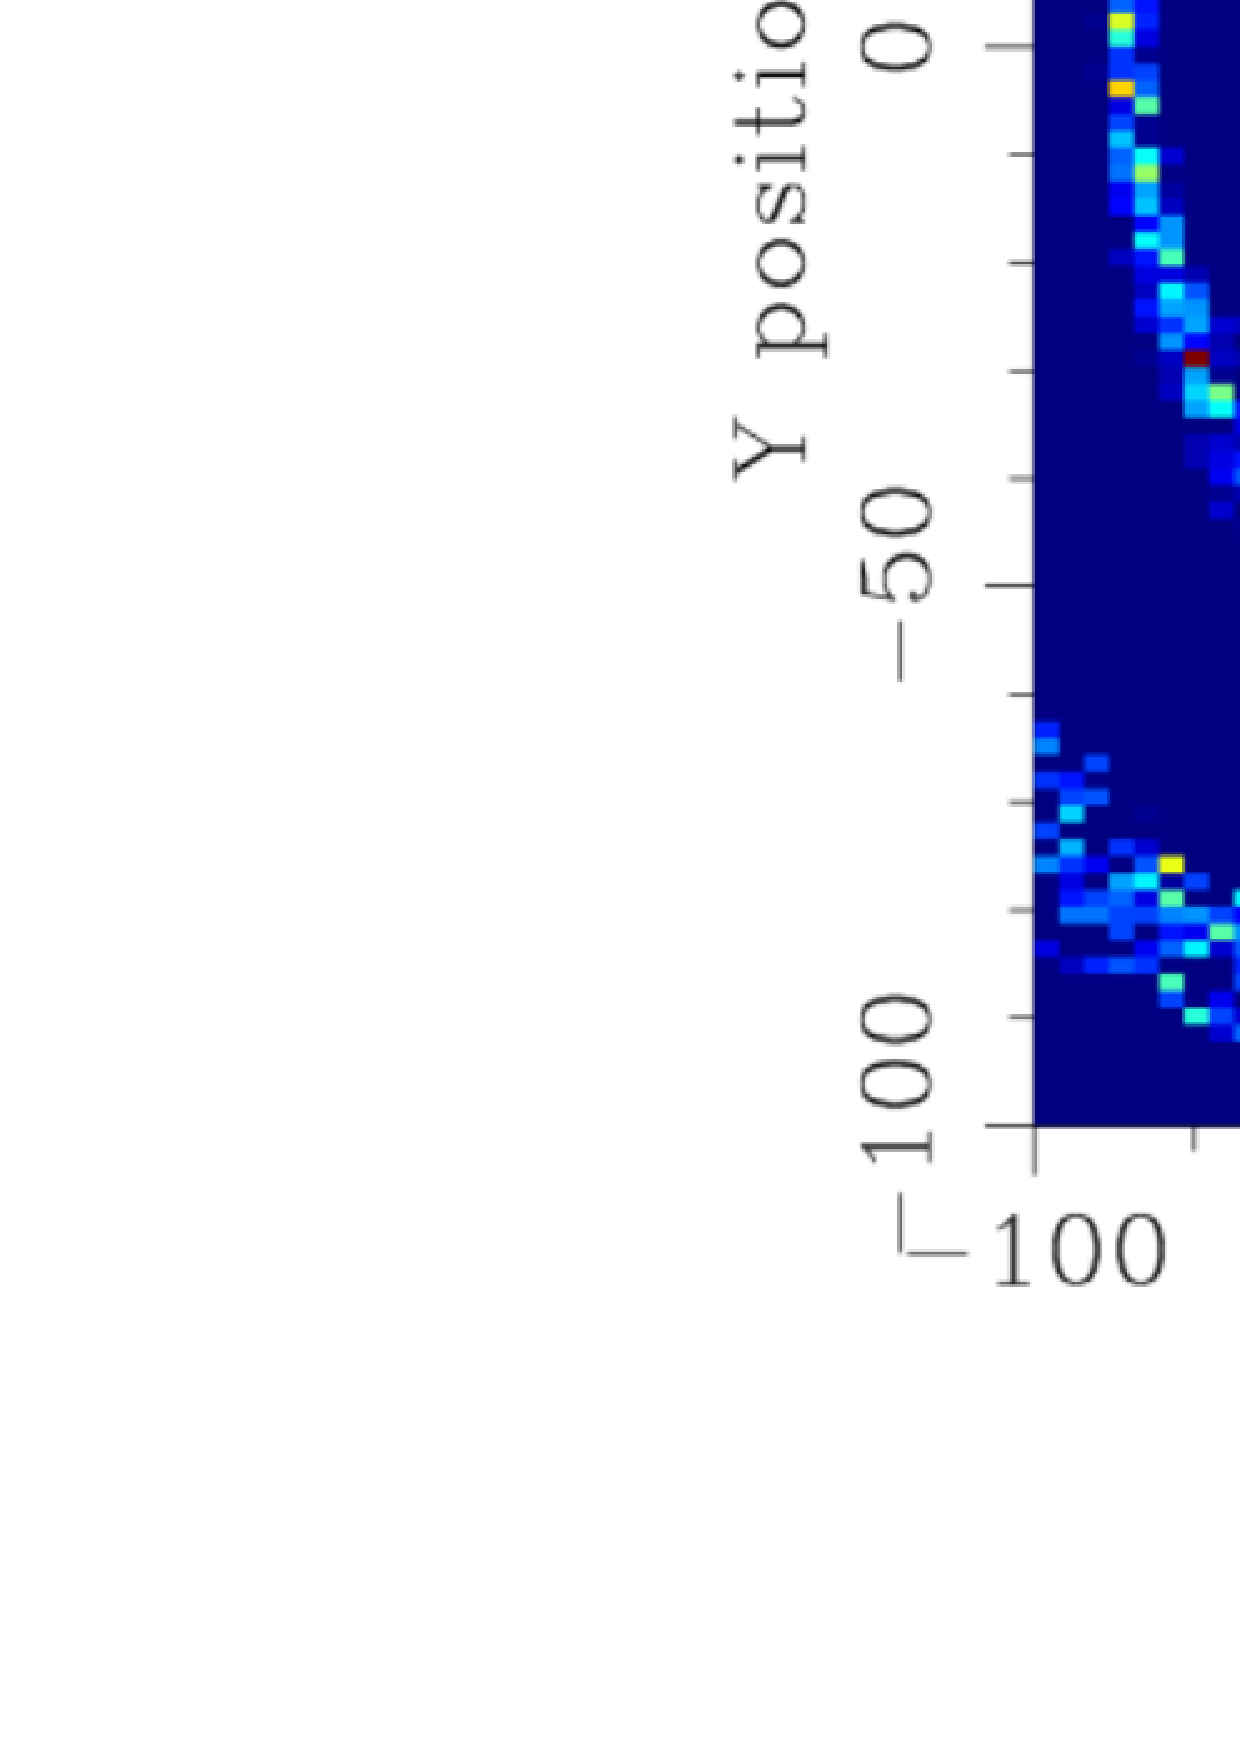
\includegraphics[width=0.95\textwidth]{figures/frontpage}
   \end{flushright}
   \par \vfill \baselineskip 12dd
 \frtnbf\noindent Ris{\o} DTU, Roskilde, Denmark \par
 \vskip 4dd \noindent\ifcase\month\or
 January\or February\or March\or April\or May\or June\or
 July\or August\or September\or October\or November\or December\fi
 \space\number\year }

\let\reportlan=\relax
\def\month{5}                   % Released in November 2005
% Need to match front page line breaking.
\title{User~and~Programmers~Guide~to~\rlap{the}\\ % Avoid overfull message.
 Neutron~Ray-Tracing~Package\\
 \MCS, Version \version\ }
\author{Peter Willendrup, Erik Knudsen, Emmanuel Farhi and\\Kim Lefmann}

\maketitle
\endgroup


\thispagestyle{empty}
% Emacs settings: -*-mode: latex; TeX-master: "manual.tex"; -*-

\begin{abstract}
The software package McStas is a tool for carrying out Monte Carlo
ray-tracing simulations of neutron scattering instruments with high
complexity and precision. The simulations can compute all aspects of the
performance of instruments and can thus be used to optimize the use of
existing equipment, design new instrumentation, and carry out virtual
experiments. McStas
is based on a unique design where an automatic compilation process
translates high-level textual instrument descriptions into efficient
ANSI-C code. This design makes it simple to set up typical simulations
and also gives essentially unlimited freedom to handle more unusual
cases.

This report constitutes the reference manual for McStas, and,
together with the manual for the McStas components, it
contains full documentation of all aspects of the program. It covers
the various ways to compile and run simulations, a description of the
meta-language used to define simulations, 
%a full description of all
%algorithms used to calculate the effects of the various optical
%components in instruments, 
and some example simulations performed with
the program.

\end{abstract}

\vskip\baselineskip\noindent
This report documents \MCS\ version \version, released \reldate
\vskip\baselineskip\noindent
The authors are:
\begin{quote}
\label{p:authors}
Kim Lefmann \verb+<kim.lefmann@risoe.dk>+ \\
Materials Research Department, Ris{\o} National Laboratory, Roskilde, Denmark 

Peter Kj\ae r Willendrup \verb+<peter.willendrup@risoe.dk>+ \\
Materials Research Department, Ris{\o} National Laboratory, Roskilde, Denmark 

Emmanuel Farhi \verb+<farhi@ill.fr>+ \\
Institut Laue-Langevin, Grenoble, France 

Mark Hagen \verb+<mhz@ansto.gov.au>+ \\
Australian Nuclear Science and technology Organization, Sydney, Australia 
\end{quote}
as well as authors who left the project:
\begin{quote}
Per-Olof {\AA}strand \verb+<per-olof.aastrand@risoe.dk>+\\
Materials Research Department, Ris{\o} National Laboratory, Roskilde, Denmark 

Kristian Nielsen \verb+<kn@sifira.dk>+ \\
Materials Research Department, Ris{\o} National Laboratory, Roskilde, Denmark 
Present address: Sifira A/S, Copenhagen, Denmark, 
\end{quote}
%Front page illustration:\\[\baselineskip]
%Simulated scattering from a vanadium sample
%taking into account the secondary extinction. See
%section~\ref{s:vanadium-result}.
\vfill
\noindent ISBN 87--550--3230--3
\par\noindent ISBN 87--550--3231--1 (Internet)
\par\noindent ISSN 0106--2840
\par\noindent\hbox{}\hfill
    Pitney Bowes Management Services Denmark A/S $\cdot$ Ris{\o} National Laboratory $\cdot$ \number\year
%    Information Service Department $\cdot$ Ris{\o} $\cdot$ \number\year
\par
\thispagestyle{empty}\clearpage





\tableofcontents

%FIXME % Emacs settings: -*-mode: latex; TeX-master: "manual.tex"; -*-

\addcontentsline{toc}{chapter}{\protect\numberline{}{Preface and acknowledgements}}
\chapter*{Preface and acknowledgements}
This document contains information on the Monte Carlo neutron
ray-tracing program \MCS\ version \version, building on the initial
release in October 1998 of version 1.0 as presented in Ref.~\cite{nn_10_20}. The reader of this
document is supposed to have some knowledge of neutron scattering,
whereas only little knowledge about simulation techniques is
required. In a few places, we also assume familiarity with the
use of the C programming language and UNIX/Linux.

It is a pleasure to thank Prof.~Kurt N.~Clausen, PSI, for his continuous
support to this project and for having initiated \MCS\ in the first
place. Essential support has also been given by Prof.~Robert McGreevy, ISIS.
Apart from the authors of this manual, also Per-Olof \AA strand, NTNU Trondheim,
has contrubuted to the development of the \MCS\ system.
%Both he and our other collaborators, Henrik M.\ R\o nnow and Mark
%Hagen have made major contributions to the project.  Also the
%contributions from our test users, the students Asger Abrahamsen, Niels
%Bech Christensen, and Erik Lauridsen, are gratefully acknowledged; they
%gave us an excellent opportunity to pinpoint a vast amount of serious
%errors in the test version.  Useful comments to this document itself
%have been given by Bella Lake and Alan Tennant.
We have also benefited
from discussions with many other people in the neutron scattering
community, too numerous to mention here.

%Philipp Bernhardt contributed the two chopper components in
%sections~\ref{s:chopper} and~\ref{s:first_chopper}. Emmanuel Farhi
%contributed the components in sections~\ref{s:sourceoptimizer},
%\ref{s:monitornd}, and~\ref{s:monitoroptimizer}. We encourage other
%users to contribute components with manual entries for inclusion in
%future versions of \MCS.

In case of errors, questions, or suggestions,
%or other need for support should arise,
do not hesitate to
contact the authors at \verb+mcstas@risoe.dk+
or consult the \MCS\ WWW home page~\cite{mcstas_webpage}.
A special bug/request reporting service is available \cite{mczilla_webpage}.

If you {\bf appreciate} this software, please subscribe to the \verb+neutron-mc@risoe.dk+ email list, send us a smiley message, and contribute to the package. We also encourage you to refer to this software when publishing results, with the following citations:
\begin{itemize}
\item{K. Lefmann and K. Nielsen, Neutron News 10/3, 20, (1999).}
\item{P. Willendrup, E. Farhi and K. Lefmann, Physica B, 350 (2004) 735.}
\end{itemize}


\section*{\MCS\ \version\ contributors}
Several people outside the core developer team have been contributing
to \MCS\ \version:
\begin{itemize}
\item{Dickon Champion and Stuart Ansell, ISIS:
    \verb+ISIS_moderator+. Dickon also contributed his model of the
    ISIS HET instrument plus a test instrument for the moderator
    component and assisted in various debugging.}
\item{Uwe Filges, PSI: \verb+Guide_tapering+ and a model of the PSI
    FOCUS instrument}
\item{Ross Stewart, ILL: New \verb+Guide_curved+}
\item{Chris Ling, ILL: ILL D9 instrument}
\item{Lise Arleth, KVL Denmark: Co-author of the \verb+Sans_spheres+ component}
\item{Geza Zsigmond helped a lot in porting his Fermi Chopper component from Vitess \cite{Vitess,vitess_webpage} to \MCS .}
\end{itemize}
Thank you guys! This is what \MCS\ is all about!

Third party software included in \MCS\ are:
\begin{itemize}
\item perl Math::Amoeba from John A.R. Williams \verb+J.A.R.Williams@aston.ac.uk+.
\item perl Tk::Codetext from Hans Jeuken \verb+haje@toneel.demon.nl+.
\item scilab Plotlib from St\'ephane Mottelet \verb+mottelet@utc.fr+.
\item and optionally PGPLOT from Tim Pearson \verb+tjp@astro.caltech.edu+.
\end{itemize}

The \MCS\ project has been supported by the European Union, initially
through the XENNI program and the RTD ``Cool Neutrons'' program in FP4,
In FP5, \MCS\ was supported strongly through the
``SCANS'' program.
Currently, in FP6, \MCS\ is supported through the Joint Research Activity
``MCNSI'' under the Integrated Infrastructure Initiative ``NMI3'', see
the WWW home pages~\cite{mcnsi_webpage,nmi3_webpage}.


% Emacs settings: -*-mode: latex; TeX-master: "manual.tex"; -*-

\chapter{Introduction to \MCS}

Efficient design and optimization of neutron spectrometers are
formidable challenges. Monte Carlo techniques are well matched to meet
these challenges. When \MCS\ version 1.0 was released in October
1998, except for the NISP/MCLib program~\cite{nisp_webpage}, no existing package offered a general framework for the neutron
scattering community to tackle the problems currently faced at reactor and
spallation sources. The \MCS\ project was designed to provide such a framework.

\MCS\ %({\em Monte Carlo Simulations of Triple Axis Spectrometers\/})
is a fast and versatile software tool for neutron ray-tracing simulations.
It is based on a meta-language specially designed for neutron
simulation. Specifications are written in this language by users and
automatically translated into efficient simulation codes in ANSI-C.
The present version supports both continuous and pulsed source instru-
ments, and includes a library of standard
components with in total around 100 components. These enable to simulate all kinds of neutron scattering instruments (diffractometers, spectrometers, reflectometers, small-angle, back-scattering,...) for both continuous and pulsed sources.

The \MCS\ package is written in ANSI-C and is freely available for down-load
from the \MCS\ web-page~\cite{mcstas_webpage}. The package is actively
being developed and supported by Ris\o\ National Laboratory
and the Institut Laue Langevin (ILL).
The system is well tested and
is supplied with several examples and with an extensive documentation.
Besides this manual, a separate component manual exists.


\section{Historical background}

In the late 90'ies at Ris\o\ National Laboratory,
simulation tools were urgently needed,
not only to better utilize existing instruments
({\em e.g.} RITA-1 and RITA-2~\cite{cjp_73_697,pb_241_50,pb_283_343}),
but also to plan completely new instruments for new sources
({\em e.g.} the Spallation Neutron Source, SNS~\cite{sns_webpage}
and the planned European Spallation Source, ESS~\cite{ess_webpage}).
Writing programs in C or Fortran for
each of the different cases involves a huge effort, with debugging presenting
particularly difficult problems. A higher level tool specially designed
for simulating neutron instruments was needed. As there was
no existing simulation software that would fulfill our needs, the \MCS\
project was initiated.
In addition, the ILL required an efficient and general simulation
package in order to achieve renewal of its instruments and guides.
A significant contribution to both the component library and the \MCS\
kernel itself was early performed at the ILL and included in the package.
ILL later became a part of the core \MCS\ team.

\section{Scientific background}
What makes scientists happy? Probably collect good quality data, pushing the instruments to their limits, and fit that data to physical models.
Among available measurement techniques, neutron scattering provides a
large variety of spectrometers to probe structure and dynamics of all
kinds of materials. 

Unfortunately the neutron flux is often a limitation in the
experiments. This then motivates instrument responsibles to improve
the flux and the overall efficiency at the spectrometer positions, and
even to design new machines. Using both analytical and numerical
methods, optimal configurations may be found. 

But achieving a satisfactory experiment on the best neutron
spectrometer is not all. Once collected, the data analysis process
raises some questions concerning the signal: what is the background
signal ? What proportion of coherent and incoherent scattering has
been measured ? Is is possible to identify clearly the purely elastic
(structure) contribution from the quasi-elastic and inelastic one
(dynamics) ? What are the contributions from the sample geometry, the
container, the sample environment, and generally the instrument itself
? And last but not least, how does multiple scattering affect the
signal ? Most of the time, the physicist will elude these questions
using rough approximations, or applying analytical corrections
\cite{Copley86}. Monte-Carlo techniques provide a mean to evaluate
some of these quantities. The techincalities of Monte-Carlo simulation
techniques are explained in detail in Chapter \ref{c:MCtechniques}.


\subsection{The goals of \MCS}
\label{s:goals}

Initially, the \MCS\ project had four main objectives
that determined its design.

\paragraph{Correctness.}
It is essential to minimize the potential for bugs in computer
simulations.  If a word processing program contains bugs, it will
produce bad-looking output or may even crash. This is a nuisance, but at
least you know that something is wrong. However, if a simulation
contains bugs it produces wrong results, and unless the results are far
off, you may not know about it! Complex simulations involve hundreds or
even thousands of lines of formulae, making debugging a major issue. Thus the
system should be designed from the start to help minimize the potential
for bugs to be introduced in the first place, and provide good tools for
testing to maximize the chances of finding existing bugs.
%
\paragraph{Flexibility.}
When you commit yourself to using a tool for an important project, you
need to know if the tool will satisfy not only your present, but also
your future requirements. The tool must not have fundamental limitations that
restrict its potential usage. Thus the \MCS\ systems needs to be
flexible enough to simulate different kinds of instruments
as well as many different kind of
optical components, and it must also be extensible so that future, as
yet unforeseen, needs can be satisfied.
%
\paragraph{Power.}
``\textit{Simple things should be simple; complex things should be possible}''.
New ideas should be easy to try out, and the time from thought to action
should be as short as possible. If you are faced with the prospect of programming for
two weeks before getting any results on a new idea, you will most likely drop
it. Ideally, if you have a good idea at lunch time, the simulation
should be running in the afternoon.
%
\paragraph{Efficiency.}
Monte Carlo simulations are computationally intensive, hardware capacities
are finite (albeit impressive), and humans are impatient. Thus the
system must assist in producing simulations that run as fast as
possible, without placing unreasonable burdens on the user in order to
achieve this.


\section{The design of \MCS}
\label{s:design}

In order to meet these ambitious goals, it was decided that \MCS\ should
be based on its own meta-language, specially designed for
simulating neutron scattering instruments. Simulations are written in
this meta-language by the user, and the \MCS\ compiler automatically
translates them into efficient simulation programs written in ANSI-C.

In realizing the design of \MCS, the task was
separated into four conceptual layers:
\begin{enumerate}
\item Modeling the physical processes of neutron scattering, \textit{i.e}.\
  the calculation of the fate of a neutron that passes through the
  individual components of the instrument (absorption, scattering at a
  particular angle, etc.)
\item Modeling of the overall instrument geometry, mainly consisting
  of the type and position of the individual components.
\item Accurate calculation, using Monte Carlo techniques, of
  instrument properties such as resolution function from the result of
  ray-tracing of a large number of neutrons. This includes estimating
  the accuracy of the calculation.
\item Presentation of the calculations, graphical or otherwise.
\end{enumerate}

Though obviously interrelated, these four layers can be
treated independently, and this is reflected in the overall system
architecture of \MCS. The user will in many situations be
interested in knowing the details only in some of the layers. For
example, one user may merely look at some results prepared by others,
without worrying about the details of the calculation. Another user
may simulate a new instrument without having to reinvent the
code for simulating the individual components in the instrument. A third
user may write an intricate simulation of a complex component,
e.g.\ a detailed description of a rotating velocity selector,
and expect other users to easily
benefit from his/her work, and so on. \MCS\ attempts to make it
possible to work at any combination of layers in isolation by separating
the layers as much as possible in the design of the system and in
the meta-language in which simulations are written.

The usage of a special meta-language and an automatic compiler has
several advantages over writing a big monolithic program or a set of
library functions in C, Fortran, or another general-purpose programming
language.  The meta-language is more \textit{powerful}; specifications
are much simpler to write and easier to read when the syntax of the
specification language reflects the problem domain. For example, the
geometry of instruments would be much more complex if it were specified
in C code with static arrays and pointers. The compiler can also take
care of the low-level details of interfacing the various parts of the
specification with the underlying C implementation language and each
other. This way, users do not need to know about \MCS\ internals to
write new component or instrument definitions, and even if those
internals change in later versions of \MCS, existing definitions can be
used without modification.

The \MCS\ system also utilizes the meta-language to let the \MCS\
compiler generate as much code as possible automatically, letting the
compiler handle some of the things that would otherwise be the task of
the user/programmer. \textit{Correctness} is improved by having a well-tested
compiler generate code that would otherwise need to be specially written
and debugged by the user for every instrument or component. \textit{Efficiency}
is also improved by letting the compiler optimize the generated code in
ways that would be time-consuming or difficult for humans to do. Furthermore, the
compiler can generate several different simulations from the same
specification, for example to optimize the simulations in different
ways, to generate a simulation that graphically displays neutron
trajectories, and possibly other things in the future that were not even
considered when the original instrument specification was written.

The design of \MCS\ makes it well suited for doing ``what if\ldots''
types of simulations. Once an instrument has been defined, questions
such as ``what if a slit was inserted'', ``what if a focusing
monochromator was used instead of a flat one'', ``what if the sample was
offset 2~mm from the center of the axis'' and so on are easy to answer. Within
minutes the instrument definition can be modified and a
new simulation program generated. It also makes it simple to debug new
components. A test instrument definition may be written
containing a neutron source, the component to be tested, and whatever
detectors are useful, and the component can be thoroughly tested before
being used in a complex simulation with many different components.

The \MCS\ system is based on ANSI-C, making it both efficient and
portable. The meta-language allows the user to embed arbitrary C code in
the specifications. \textit{Flexibility} is thus ensured since the full
power of the C language is available if needed.


\section{Overview}

The \MCS\ system documentation consists of the following major
parts:
\begin{itemize}
\item A short list of new features introduced in this \MCS\ release
  appears in chapter~\ref{c:changes}
\item Chapter~\ref{s:install} explains how to obtain, compile
  and install the \MCS\ compiler, associated files and supportive software
\item Chapter~\ref{s:MCtechniques} concerns Monte Carlo techniques
  and simulation strategies in general
\item Chapter~\ref{c:running} includes a brief introduction to the
  \MCS\ system 
  (section~\ref{s:brief}) as well a section (\ref{s:running}) on running the compiler to produce
  simulations. Section~\ref{s:run-sim} explains how to run the generated
  simulations. Running \MCS\ on parallel computers require special
  attention and is discussed in section~\ref{s:run-mpi}. A number of front-end programs are used to run the
  simulations and to aid in the data collection and analysis of the
  results. These user interfaces are described in section~\ref{s:frontends}.
\item The \MCS\ meta-language is described in chapter~\ref{s:kernel}. This
  chapter also describes a set of library functions and definitions
  that aid in the writing of simulations. See
  appendix~\ref{c:kernelcalls} for more details.
\item The \MCS\ component library contains a collection of
  well-tested, as well as user contributed, beam components that can be used in simulations.
  The \MCS\ component library is documented in a separate manual
  and on the \MCS\ web-page~\cite{mcstas_webpage}, but a short overview of these
  components is given in chapter~\ref{s:components} of the Manual.
  %This
  %library is documented in detail in chapter~\ref{s:components}. Code
  %for the components can be found in appendix~\ref{compcode}.
\item A collection of example instrument definitions is described in
  chapter~\ref{s:instrument} of the Manual.%, with source code given in appendix~\ref{instcode}.

\end{itemize}

%In addition, some results from
%simulations with \MCS\ are described in
%appendix~\ref{testresults}.
A list of library calls that may be used in component definitions
appears in appendix~\ref{c:kernelcalls}, and
an explanation of the \MCS\ terminology can be
found in appendix~\ref{s:terminology} of the Manual..
Plans for future extensions are presented on the \MCS\ web-page~\cite{mcstas_webpage} as well as in section~\ref{s:future}.


%The \MCS\ package consists of four levels:
%\paragraph{The kernel.} Here are located some geometrical tools
%({\em e.g.} intersection between a line and various surfaces)
%and other elemental tools ({\em e.g.} creation and annihilation
%of a neutron). The kernel is maintained by the Ris\o\ group.

%\paragraph{The components.} Here resides the code for simulation
% of the individual spectrometer components
% (sources, detectors, samples, and optical elements).
% Components may have input parameters, like the angle of divergence of a
% collimator or the mosaicity of a monochromator crystal.
% Interested users are encouraged to modify existing components and to
% design new ones.
% A library of general and well documented components
% is being maintained by the Ris\o\ group.

%\paragraph{The instruments.} An instrument definition is written
% in the \MCS\ meta-language, which is a means of positioning
% components within an experimental geometry.
% Instruments may have inout parameters, like {\em e.g.}\ the three
% $(\omega,2\theta)$ pairs of a standard triple-axis spectrometer.
% For each specific instrument, a new instrument definition
% should be written. This will usually be done by the users,
% possibly in collaboration with the Ris\o\ group.

%\paragraph{The instrument control interface.}
% Here, the setting parameters of the
% instrument may be controlled in order to perform a simulation series.

% In the present version 1.0, the control interface
% consists of a very preliminary MATLAB program,
% but we expect soon to implement a simulation version of the
% Ris\o\ spectrometer control software TASCOM.
% By using the preprogrammed scans or the TASCOM programming features,
% the user will then be able easily to perform the desired simulations.
% Later, interfaces to other control software may be implemented.

%\paragraph{Data analysis and visualization}
% The output data is in the present version written as
% plain ASCII format, but will later be written in the TASCOM format,
% from where it may easily be converted into the general
% NeXus format\cite{NeXus}.
% This enables the user to choose between various analysis packages
% for the output side.
% Both ASCII and TASCOM files may be analysed and plotted through
% the Ris\o\ MATLAB package MVIEW/MFIT \cite{mview}.

% Emacs settings: -*-mode: latex; TeX-master: "manual.tex"; -*-

\chapter{New features in \MCS\ versions 1.7 - \version\ }
\label{c:changes}

Many new features have been implemented in \MCS\ version \version\  since
version 1.5 (no version 1.6. manual was written, the most important being that
\MCS\ can now compile and run in a Windows enviroment.  The list of changes
given here may be particularly  useful to experienced \MCS\ users who do not
wish to read the whole  manual, searching only for new features. A global
upward compatibility  exists for all changes, and thus all previous components
and  instruments should work as before. Changes are labelled as 1.7 or 1.8 to 
indicate in which \MCS\ version they appeared.

Important note for Windows users: It is a known problem that some of
the \MCS\ tools do not support filenames / directories with spaces.
We are working on a more general approach to this problem, which will
hopefully be solved in the next release.

\section{General}
\label{s:new-features:general}
As of \MCS\ version \version\, the license covering the \MCS\ package
is the GNU General Pubclic License. See \verb+http://www.gnu.org+ for details.

\section{Kernel} 
\label{s:new-features:kernel}
\index{Kernel}

The following changes concern the 'Kernel' (i.e. the \MCS\ meta-language and program). See the dedicated chapter in the {\it User manual} for more details.

\begin{itemize}
\item \MCS\ can now compile for Windows!
\item Instrument parameters may now have default values, the same way as components do 
    (appeared in 1.8). \index{Parameters!Optional, default value}
\item An instrument source file may contain \texttt{EXTEND} \%\{ \ldots \}\% C
    blocks just after the usual \texttt{AT} \ldots \texttt{ROTATED} \ldots
    keywords, to extend the behaviour of existing components, without touching
    their code. All local component variables are  available. This may for
    instance be used to add a new 'color' to neutrons,  i.e. assign a new
    characteristic variable to the neutron (appeared in 1.7).
    \index{Keyword!EXTEND}
\item Component instances in an instrument file may be \texttt{GROUP}'ed into 
    exclusive assembly, i.e.\ only one component of the group will intercept
    the neutron ray, the rest will be skipped. This is useful for multi
    monochromators multi detectors, multiple collimators, etc.  After the
    \texttt{ROTATED} keyword, the keyword \texttt{GROUP} should be added
    followed by a group name (e.g. \texttt{GROUP} MyGroup)  (appeared in 1.7).
    \index{Keyword!GROUP}    
\item The instrument and components may have string (\verb+char*+) setting
    parameters. For components, their length is limited to 1024 characters
    (appeared in 1.7). \index{Parameters!Instruments} \index{Parameters!Setting}
\item In both components and instruments, the \texttt{FINALLY} section, that is
    executed at the end of simulations, has been supplemented with a new
    \texttt{SAVE} section. This latter is executed at simulation end (just
    before the \texttt{FINALLY} section), but also each time an intermediate
    save is required (e.g.\   when a 'kill -USR2 \$pid' is used under Unix, see
    section \ref{s:new-features:run-time})  (appeared in 1.7). 
    \index{Keyword!SAVE} \index{Keyword!FINALLY} \index{Signal handler!USR2 signal}
\item Components may have a \texttt{SHARE} section, which is imported only once
    per type of component. \texttt{SHARE} has the same role as
    \texttt{DECLARE}, but is useful when several instances of the same
    component is used in a single simulation  (appeared in 1.7).
    \index{Keyword!SHARE} \index{Keyword!DECLARE}
\item The component files may have some \texttt{\%include} inside '\%\{ \}\%'
    \texttt{DECLARE} or \texttt{SHARE} C blocks. The files to include are
    searched locally, and then in the library. If an extension is found, only
    the specified file is included, else both  .h and .c are embedded unless
    the --no-runtime has been specified. As in previous releases, the
    instrument files can embed external files, both in C blocks  and in the
    instrument parts (\texttt{DECLARE}, etc.) (appeared in 1.7).
    \index{Keyword!%include}
\item The \texttt{PREVIOUS} keyword, to be used after \texttt{RELATIVE} in
    place of component instance names refers to the preceeding component, and
    does not require to actually know  its name. Similarly the
    \texttt{PREVIOUS(n)} keyword refers to the $n$-th preceeding component
    (appeared in 1.8). \index{Keyword!PREVIOUS}
\end{itemize}

\section{Run-time} 
\label{s:new-features:run-time}
\index{Library!Run-time}

Some important modifications were done to the 'Run-time' library 
(i.e.\ the functions used in the instrument program). 
Some details may be found in {\it Running} chapter of the {\it User manual}
as well as in the appendix~\ref{c:kernelcalls}.

\begin{itemize}
\item A global gravitation handling is now available, by setting the \verb+-g+ flag.
\item Many output formats are available for data. Use the
    \verb+--format="format"+ flag, e.g. \verb+--format="Scilab"+.  The default
    format is McStas/PGPLOT, but may be specified globally using the
    \verb+MCSTAS_FORMAT+ environment variable.  See section~\ref{s:run-format}
    for details (appeared in 1.7). \index{Environment variable!MCSTAS\_FORMAT}
    \index{Data format}
\item It is possible to save 3D data arrays, by calling the DETECTOR\_OUT\_3D
    macro. (handled as 2D by \verb+mcplot+ by ignoring the 3rd dimension)
    (appeared in 1.7).  \index{Library!Run-time!DETECTOR\_OUT}
\item The C type of the 'number of events' array in monitors (usually named
    \verb+L_N+) was changed from \verb+int+ to \verb+double+, to avoid overflow.
    All 'home-made' monitors should be updated accordingly (appeared in 1.7).
\item The \verb+USR2+ signal generates an intermediate save for all monitors,
    during the simulation (executes the \texttt{SAVE} section). The \verb+USR1+
    signal still gives informations (appeared in 1.7). \index{Signal handler!USR1 signal}
\item New \verb+randvec_target_rect+ and \verb+randvec_target_rect_angular+
    functions now focus  on a rectangle (more efficient than the former
    \verb+randvec_target_sphere+) (appeared in 1.7 and 1.8).
    \index{Library!Run-time!randvec\_target\_rect}
\end{itemize}


\section{Components and Library} 
\label{s:new-features:components}
\index{Components} \index{Library!Components}
  
  We here list some of the new components (found in the \MCS\ \verb+lib+ directory) 
which are detailed in the {\it Component manual}, also mentioned in
the {\it Component Overview} of the {\it User Manual}.
  
\begin{itemize}
\item All components now have a valid header for \texttt{mcdoc} automatic documentation, as well as usage example.
\item \texttt{contrib} This directory now contains contributed
    components. Those that will be found to be highly stable will then
    go into the other component categories. Contributed components
    (\verb+Guide_honeycomb+, \verb+Guide_tapering+,
    \verb+Guide_curved+, \verb+ISIS_moderator+) have been
    placed there (appeared in 1.7 and 1.8). \index{Library!Components!contrib}
\item \texttt{data} This directory now contains example data files mainly for Laue diffraction, transmission and reflection files. \index{Library!Components!data}
\item \texttt{doc} The documentation is now included in the \verb+doc+ directory. \index{Library!Components!doc}
\item \texttt{example} A new \verb+example+ directory contains instrument examples, available from the \verb+mcgui+ 'Neutron site' menu Tool.\index{Library!Instruments}
\item \texttt{misc} Updated \verb+Vitess_input+ and \verb+Vitess_output+ components according to Vitess >= 2.3 Neutron structure.\index{Library!Components!misc}
\item \texttt{misc} A \verb+Progress_bar+ component may be positioned anywhere in the simulation and displays the simulation percentage. It may also save temporary data files regularly so that one can have a look \index{Tools!mcplot} (using \verb+mcplot+) at the results on-the-fly before the end of the simulation.
\item \texttt{monitors} The \verb+Monitor_nD+ component may be used as a replacement for all monitors. It may have automatic limits mode for either all or selected monitored variables. It may also plot banana monitors for \verb+mcdisplay+ and monitor something else than the intensity, e.g. the mean energy on a XY psd (appeared in 1.7). \index{Library!Components!monitors} A bug (atan2) was corrected in \verb+PSD_monitor_4PI+. \index{Library!Components!monitors}
\item \texttt{obsolete} Some components were renamed by categories for better sorting. Old components are still available, but not maintained anymore. We highly encourage to avoid using these when writing new instrument definitions. \index{Library!Components!obsolete}
\item \texttt{optics} components were renamed by categories, starting with
   Guide\_\ldots, Monochromator\_\ldots, Filter\_\ldots etc so that sorting is
   easier (appeared in 1.7). \index{Library!Components!optics}
\item \texttt{optics} Monochromator\_curved can read reflectivity and transmission tables (appeared in 1.7).   
\item \texttt{optics} Guide\_gravity can handle a 2D array of channels, and
    has options for subdivisions in length, chamfers and wavyness.
\item \texttt{optics} Filter\_gen can read a table from a file and affect the neutron
    beam (replaces the obsolete \verb+Flux_adapter+). It may act as a filter or a
    source (appeared in 1.7).    
\item \texttt{optics} Bugs were corrected in the following components: Bender, Chopper, Guide\_channeled. Some similar components were gathered. New components were added: Guide\_gravity, Guide\_wavy, Filter\_gen. \index{Library!Components!optics}
\item \texttt{samples} can now target towards any component, given its index 
    (no need to compute \verb+target_x|y|z+ vector, use e.g. \verb+target_index=1+). 
    Position an \verb+Arm+ at the focusing position when targetting to 
    centered components (appeared in 1.7). \index{Library!Components!samples}
\item \texttt{samples} Rectangular focusing has been implemented
  (instead of circular) in most components. More sample shapes are
  available. A bug has been corrected in Single\_crystal. A Powder2
  component (2 rings) has been added. Sans\_spheres is a new sample
  component for small angle scattering. Phonon\_simple is a new sample
  for phonon scattering. (appeared in 1.8). \index{Library!Components!samples}
\item \texttt{share} Many dedicated libraries are now available as shared code for reading tables,
    handling data files and monitors. These are C functions to be \texttt{\%include}d
    into components (see e.g. \verb+MCSTAS/monitors/Monitor_nD.comp+) (appeared in 1.7).
    \index{Library!Components!share}
\item \texttt{sources} The \verb+Source_gen+ and \verb+Source_Maxwell_3+ components may now simulate all kinds of continuous neutron sources. Some bugs were corrected in most sources in order to have an isotropic neutron emission. The \verb+Virtual_input+ and \verb+Virtual_output+ may load and save neutron event files (beware the size of the generated files !). Format may be text or binary (appeared in 1.7). \index{Library!Components!sources}
\end{itemize}

\section{Documentation}
\label{s:new-features:documentation}
As of \MCS\ \version\ an improved tutorial has been integrated
into to the graphical user interface of \MCS\. The content of the
tutorial is also available in appendix \ref{tutorial}.

\section{Example instruments}
\label{s:new-features:instruments}
As mentioned above, \MCS\ \version\ has various improvements regarding
distribution of instruments. Firstly, \verb+mcgui+ has a new special
menu for instruments distributed with \MCS and secondly instruments can
now have default values and thirdly a new \MCS\ tutorial has
integrated into the user interface. These three new features together
proves a solid starting point for new users of \MCS\. To further
increase the value of the package, we have decided to include selveral
example instruments contributed by \MCS\ users. The full list of 
example instruments are
\begin{itemize}
\item{\verb+vanadium_example+, improved version used in the \MCS\
    tutorial.}
\item{\verb+linup-1+-\verb+linup-7+, legacy instruments of the Ris\o\
    TAS1 instrument from a historical release of \MCS.}
\item{\verb+h8_test+, model of the Brookhaven H8 triple-axis, written
    by McStas team member Emmanuel Farhi}
\item{\verb+ILL_D9+, a model of the ILL D9 hot four-circle
    diffractometer, contributed by Chris Ling}
\item{\verb+Hetfull+, a model of the ISIS HET spectrometer,
    contributed by Dickon Champion}
\item{\verb+focus_psi+, a model of the PSI FOCUS spectrometer,
    contributed by Uwe Filges}
\item{\verb+prisma2+, a model of the ISIS prisma2 spectrometer,
    written by Kristian Nielsen and Mark Hagen from a historical release of \MCS.}
\item{Test instruments \verb+ISIStest+ for testing the new
    \verb+ISIS_moderator+ component, \verb+SANS+ for testing the new
    \verb+Sans_spheres+ component and \verb+Test_Phonon+ for testing
    the new \verb+Phonon_simple+ component, all contributed by the
    corresponding component authors.} 
\end{itemize}



\section{Tools, installation}
\label{s:new-features:tools}
\index{Tools}
\index{Installing}
  A renewal of most \MCS\ Tools, used to edit and display instrument or
  results,  has been undertaken, aiming at proposing alternatives to the
  Perl+PerlTk+PGPLOT+PDL  libraries.
  
  Quite a lot of work was achieved in order to solve the installation problems
   that have been encoutered so far. A fully working \MCS\ distribution now
   only requires a C compiler, perl, perl-Tk and one of Matlab, Scilab and
   (PGPLOT, perl-DL). The Plotlib Scilab library has  been included in the
   package, and does not need to be installed separately anymore.
  
  This has improved significantly the portability of \MCS\ and thus simplified
  the installation of the package. Details about the installation and the
  available tools are given in the {\it Installing \MCS} chapter of the {\it User Manual}.

\begin{itemize}
\item The list of required packages for a complete \MCS\ installation is now a C
    compiler, Perl, PerlTk and Scilab or Matlab.
\item Matlab, Scilab and IDL may read directly McStas results if the simulation
    was executed with the \verb+--format="..."+ option 
    (see~\ref{s:new-features:run-time} changes). The former PGPLOT interface is
    still supported (appeared in 1.7).  \index{Tools!Matlab}
    \index{Tools!Scilab}  \index{Tools!IDL} \index{Tools!Perl libraries}   
\item\verb+mcgui+ can now perform \verb+mcrun+-like parameter scans
    directly from the gui (appeared in 1.8).
\item\verb+mcgui+ has now a 'Neutron site' menu which enables to load directly one of the
    instrument examples (appeared in 1.8).
\item \verb+mcrun+ can generate scan results in all formats (appeared in 1.8). 
   \index{Tools!mcrun}
\item \verb+mcrun+ has a \MCS\ self test procedure available (appeared in 1.8). 
   \index{Tools!mcrun}
\item \verb+mcplot+, \verb+mcdisplay+, \verb+mcgui+ are now less dependent on the
    \verb+perl/PDL/pgplot+ installed versions and fully work with Matlab/Scilab (appeared in 1.7). \index{Tools!mcplot}
\item \verb+mcplot+ can plot a single simulation data file.
\item \verb+mcplot+, \verb+mcresplot+, \verb+mcdisplay+ can output GIF, PS and color
    PS files. They also have integrated help (-h options), and may generate output
    files in a non interactive mode (read data, create output file, exit) (appeared in 1.7).
\item \verb+mcplot+ and \verb+mcdisplay+ work with Matlab, PGPLOT and Scilab plotters
   (depends on the \verb+MCSTAS_FORMAT+ environment variable, or -pPLOTTER option, or
   PGPLOT if not set) (appeared in 1.7).
\item \verb+mcplot+ may display parameter scan step results in all formats
   (appeared in 1.8).  \index{Tools!mcplot}
\item \verb+mcstas2vitess+ enables to convert a McStas component into a
   Vitess~\cite{vitess_webpage} one (appeared in 1.7). \index{Tools!mcstas2vitess}
\item \verb+mcresplot+ can plot projections of the 4D resolution function of an 
   instrument obtained from the \verb+Res_sample+ and \verb+Res_monitor+ components.
   In version \version, it only works with the McStas/PGPLOT format, 
   but a port for Scilab/Matlab is under way (appeared in 1.7). \index{Tools!mcresplot}
\item \verb+mcdoc+ can now display the pdf version of the manual, an
  HTML catalog of the current library, as well as help for single
  components. \index{Tools!mcdoc} The \verb+mcdoc+ functions have been
  closely integrated into \verb+mcgui+ (appeared in 1.7). 
\item \verb+mcdoc+ can document automatically instruments in the same way as components
 (appeared in 1.8).
\item \verb+mcconvert+ is a new tool to convert \MCS\ result text files from Matlab to Scilab, 
  and from Scilab to Matlab formats (appeared in 1.8). \index{Tools!mcconvert}
\end{itemize}

\section{Future extensions}
\label{s:future}
The following features are planned for the oncoming releases of \MCS :
\begin{itemize}
\item Support for Matlab and Scilab in \verb+mcresplot+.
\item Support for MPI (parallel processing library) in the runtime
\item Language extension 'JUMP' for enabeling loops, 'teleporting'
  etc. in instrument descriptions.
\item Concentric components.
\item Polarised components and magnetic field computation components.
\item Optimize a set of parameters for a better flux and/or resolution on a given monitor.
\end{itemize}









\chapter{Installing \MCS}
\label{installing}
\index{Environment variable!MCSTAS\_CC}
\index{Environment variable!MCSTAS\_CFLAGS}
\index{Environment variable!MCSTAS\_FORMAT}
\index{Testing the distribution}
\index{Installing}
The information in this chapter is also available as a separate
html/ps/pdf document in the \texttt{install\_docs/} folder of your
\MCS\ installation package.
\input{../mcstas/install_docs/tex/install_meat.tex}

% Emacs settings: -*-mode: latex; TeX-master: "manual.tex"; -*-

\chapter{Monte Carlo Techniques and simulation strategy}
\label{s:MCtechniques}

This chapter explains the simulation strategy and the Monte Carlo
techniques used in \MCS. We first explain the concept of the neutron
weight factor, and discuss the statistical errors in dealing with sums
of neutron weights.  Secondly, we give an expression for how the weight
factor should transform under a Monte Carlo choice and specialize this
to the concept of focusing components.  Finally, we present a way of
generating random numbers with arbitrary distributions.

\section{The neutron weight, $p$}
\label{s:probweight}
A totally realistic semi-classical simulation will require that
each neutron is at any time either present or not
(it might be ABSORB'ed or lost in another way).
In many set-ups, {\em e.g.} triple axis spectrometers, only a
small fraction of the initial neutrons will ever be detected, and
simulations of this kind will therefore waste much time in dealing
with neutrons that get lost.

An important way of speeding up calculations is to introduce
a neutron weight for each simulated neutron and to
adjust this weight according to the path of the neutron.
If {\em e.g.}\ the reflectivity of a certain 
optical component is 10\%, and only reflected neutrons are
considered in the simulations, the neutron
weight will be multiplied by 0.10 when passing this component,
but every neutron is allowed to reflect in the component.
In contrast, the totally realistic simulation of the component
would require in average ten incoming neutrons for each reflected one.

Let the initial neutron weight be $p_0$ and let us denote the weight
multiplication factor in the $j$'th component by $\pi_j$.  The resulting
weight factor for the neutron after passage of the whole instrument is 
equal to the product of all the contributions
\begin{equation}
\label{e:probprod}
p = p_0 \prod_{j=1}^n \pi_j .
\end{equation}
For convenience, the value of $p$ is updated within each component.

Simulation by weight adjustment is performed
whenever possible. This includes
\begin{itemize}
\item Transmission through filter.
\item Transmission through Soller blade collimator
 (in the approximation
 which does not take each blade into account).
\item Reflection from monochromator (and analyser) crystals
 with finite reflectivity and mosaicity.
\item Scattering from samples.
\end{itemize}

\subsection{Statistical errors of non-integer counts}
\label{s:staterror}

In a typical simulation, the result will consist of a
count of neutrons with different weights.\footnote{The
sum of these weights is an estimate of 
the mean number of neutrons hitting the monitor 
(or detector) in a ``real'' experiment
where the number of neutrons emitted from the source
is the same as the number of simulated neutrons.}
One may write the counting result as
\begin{equation}
\label{psum}
I = \sum_i p_i = N \overline{p} ,
\end{equation}
where $N$ is the number of neutrons in the detector and the vertical bar denote
averaging.
By performing the weight transformations, the (statistical) 
mean value of $I$ is unchanged.
However, $N$ will in general be enhanced, 
and this will improve the statistics of the simulation.

To give some estimate of the statistical error, we proceed as follows:
Let us first for simplicity assume that all the counted neutron weights are
almost equal, $p_i \approx \overline{p}$, 
and that we observe a large number of neutrons, $N \geq 10$.
Then $N$ almost follows a normal distribution
with the uncertainty $\sigma(N) = \sqrt{N}$ 
\footnote{This is not correct in a
situation where the detector counts a large fraction of the
neutrons in the simulation, but we will neglect that for now.}.
Hence, the statistical uncertainty of the observed intensity becomes
\begin{equation}
 \sigma(I) = \sqrt{N} \overline{p} = I / \sqrt{N} ,
\end{equation}
as is used in real neutron experiments (where $\overline{p} \equiv 1$).
For a better approximation we return to Eq.~(\ref{psum}).
Allowing variations in both $N$ and $\overline{p}$,
we calculate the variance of the resulting intensity,
assuming that the two variables are independent and both follow
a Gaussian distribution.
\begin{equation}
\sigma^2(I) = \sigma^2(N) \overline{p}^2 + N^2 \sigma^2(\overline{p})
            = N \overline{p}^2 + N^2 \sigma^2(\overline{p}) .
\end{equation}
Assuming that the individual weights, $p_i$, follow a Gaussian distribution
(which in many cases is far from the truth)
we have $N^2 \sigma^2(\overline{p}) = \sigma^2(\sum_i p_i) = N
\sigma^2(p_i)$
and reach
\begin{equation}
\sigma^2(I) = N \left( \overline{p}^2 + \sigma^2(p_i) \right).
\end{equation}
The statistical variance of the $p_i$'s is estimated by
$\sigma^2(p_i) \approx (N-1)^{-1} (\sum_i p_i^2 - N \overline{p}^2)$.
The resulting variance then reads
\begin{equation}
\sigma^2(I) = \frac{N}{N-1} \left( \sum_i p_i^2 - \overline{p}^2  \right) .
\end{equation}
For large values of $N$, this is very well approximated 
by the simple expression 
\begin{equation}
\sigma^2(I) \approx \sum_i p_i^2 .
\end{equation}

In order to compute the intensities and uncertainties, the detector components 
in \MCS\ thus must keep track of
$N=\sum_i p_i^0, I=\sum_i p_i^1$, and $M_2 = \sum_i p_i^2$.

\section{Weight factor transformations during a Monte Carlo
 choice}
When a Monte Carlo choice must be performed, {\em e.g.} when the
initial energy and direction of the neutron is decided at the source,
it is important to adjust the neutron weight so that the combined
effect of neutron weight change and Monte Carlo probability
equals the actual physical properties of the component.

Let us follow up on the example of a source.
In the ``real'' semi-classical world, there is a distribution
(probability density) for the neutrons in the six dimensional
(energy, direction, position) space of
$\Pi(E,\Ombold,{\bf r}) = dP/(dE d\Ombold d^3{\bf r})$ depending upon
the source temperature, geometry {\em etc.}\ In the
Monte Carlo simulations, the six coordinates are for efficiency reasons
in general picked from another distribution:
$f_{\rm MC}(E,\Ombold,{\bf r}) \neq \Pi(E, \Ombold,{\bf r})$,
since one would {\em e.g.} often generate
only neutrons within a certain parameter interval.
However, we must then require that the weights are adjusted
by a factor $\pi_j$ (in this case: $j=1$) so that
\begin{equation} \label{probrule}
f_{\rm MC}(E,\Ombold,{\bf r}) \pi_j(E,\Ombold,{\bf r})
 = \Pi(E,\Ombold,{\bf r}) .
\end{equation}
For the sources present in version \version, 
only the $(\Ombold, {\bf r})$ dependence of the correction factors
are taken into account.

The weight factor transformation rule Eq.~(\ref{probrule})
is of course also valid for other types of Monte Carlo choices,
although the probability distributions may depend upon 
different parameters. An important example 
is elastic scattering from a powder sample,
where the Monte-Carlo choices are the scattering position
and the final neutron direction.

It should be noted that the $\pi_j$'s found in the weight factor 
transformation are multiplied by the $\pi_j$'s found by the
weight adjustments described in
subsection \ref{s:probweight} to yield the final neutron
weight given by Eq.~(\ref{e:probprod}).

\subsection{Focusing components}
\label{s:focus}
An important application of weight transformation is focusing.
Assume that the sample scatters the neutrons in many directions.
In general, only neutrons flying in some of these directions will
stand any chance of being detected. These directions we call
the {\em interesting directions}.
The idea in focusing is to avoid wasting computation time on
neutrons scattered in the uninteresting directions. 
This trick is an instance of what in Monte Carlo terminology
is known as {\em importance sampling}. % \cite{importance}.

If {\em e.g.} a sample scatters isotropically 
over the whole $4\pi$ solid angle, and all interesting
directions are known to be contained within a certain 
solid angle interval $\Delta \Ombold$, only these solid angles 
are used for the Monte Carlo choice of scattering direction. 
According to Eq.~(\ref{probrule}), the weight factor will then have
to be changed by the (fixed) amount 
$\pi_j = |\Delta \Ombold| / (4 \pi)$.
One thus ensures that the mean simulated intensity is unchanged
during a "correct" focusing, while a too narrow focusing will
result in a lower (\textit{i.e.} wrong) intensity, since one cuts
away neutrons that would otherwise have counted.

One could also think of using adaptive importance sampling, % \cite{importance},
so that \MCS\ during the simulations will determine 
the most interesting directions and gradually change 
the focusing according to that. A first implementation of this idea is
found in the Source\_adapt component.%, described in section~\ref{s:Source_adapt}.

\section{Transformation of random numbers}
In order to perform the Monte Carlo choices, one needs to be able to 
pick a random number from a given distribution. However, most
random number generators only give
uniform distributions over a certain interval.
We thus need to be able to transform between probability distributions,
and we here give a short explanation on how to do this.

Assume that we pick a random number, $x$, from a distribution $\phi(x)$.
We are now interested in the shape of the distribution of the
transformed $y=f(x)$, assuming $f(x)$ is monotonous. 
All random numbers lying in the interval $[x; x+dx]$
are transformed to lie within the interval $[y; y+f'(x)dx]$, so the
resulting distribution must be $\phi(y) = \phi(x) / f'(x)$.

If the random number generator selects numbers uniformly in the interval
$[0; 1]$, we have $\phi(x) = 1$, and
one may evaluate the above expression further
\begin{equation}
\phi(y) = \frac{1}{f'(x)} = \frac{d}{dy} f^{-1}(y) . 
\end{equation}
By indefinite integration we reach
\begin{equation}
\label{e:randtrans}
\int \phi(y) dy = f^{-1}(y) = x ,
\end{equation}
which is the essential formula for finding the right transformation
of the initial random numbers.
Let us illustrate with a few examples of transformations used within the
\MCS\ components. 

\paragraph{The circle}
For finding a random point within the
circle of radius $R$, one would like to choose the polar angle from a uniform
distribution in $[0; 2\pi]$ and the radius from the normalised distribution
$\phi(r)=2r/R^2$. 
The polar angle is found simply by multiplying a random number
with $2\pi$. For the radius, we like to find $r=f(x)$, where again $x$
is the generated random number. Left side of Eq.~(\ref{e:randtrans}) gives
$\int \phi(r) dr = \int 2 r/R^2 dr = r^2/R^2$, which should equal $x$.
Hence $r = R\sqrt{x}$.


\paragraph{Exponential decay}
In a simple time-of-flight source, the neutron flux decays exponentially
after the initial activation at $t=0$. We thus want to pick an initial
neutron emission time from the normalised distribution 
$\phi(t) = \exp(-t/\tau) / \tau$.
Use of Eq.~(\ref{e:randtrans}) gives
$x = - \exp(-t/\tau)$, which is a number in the interval $[-1; 0]$.
If we want to pick a positive random number instead, we will have 
to change sign by $x_1 = -x$ and thus reach $t = - \tau \ln (x_1)$. 


\paragraph{The sphere}
For finding a random point on the surface of the unit sphere, 
one needs to determine the two angles, $(\theta, \psi)$. 
As for a circle, $\psi$ is chosen from a uniform distribution
in $[0; 2\pi]$. The probability distribution of $\theta$ should be
$\phi(\theta)=\sin(\theta)$ (for $\theta \in [0; \pi/2 ]$), 
whence $\theta=\cos^{-1}(x)$.

% Emacs settings: -*-mode: latex; TeX-master: "manual.tex"; -*-

\chapter{Running \MCS}
\label{c:running}
This chapter describes usage of the McStas simulation package. Refer
to Chapter \ref{s:install} for installation instructions. In case of
problems regarding installation or usage, the McStas mailing
list~\cite{mcstas_webpage} or the authors should be contacted.

{\bf Important note for Windows users:} It is a known problem that some of
the \MCS\ tools do not support filenames / directories with spaces.
We are working on a more general approach to this problem, which will
hopefully be solved in the next release. Also, there are known issues for \MCS\ with recent Perl versions for Windows. We recommand to use ActiveState {\bf Perl 5.6}.

To use \MCS, an instrument
definition file describing the instrument to be simulated must be
written. Alternatively, an example instrument file can be obtained
from the \verb+examples/+ directory in the distribution or from
another source.

The structure of \MCS\ is illustrated in Figure~\ref{fig:structure}.

The input files (instrument and component files) are written in the \MCS\
meta-language and are edited either by using your favourite editor
or by using the built in editor of the graphical user interface
(\texttt{mcgui}).

Next, the instrument and component files are compiled using the \MCS\ compiler
using the FLEX and Bison facilities to produce a C program\footnote{Note that
since release 1.7 of \MCS, FLEX and Bison need not be installed
on your computer.}.

The resulting C program can then be
compiled with a C compiler and run in combination with various
front-end programs for example to present the intensity at the
detector as a motor position is varied.

The output data may be analyzed in the same way as regular experiments
are analyzed by using Matlab, Scilab~\cite{scilab_webpage} or IDL or by using the Perl routines included in \MCS .\index{Tools}

\begin{figure}[htb!]
\begin{center}
%\documentclass{article}
%\usepackage{pstricks,pst-node}

%\begin{document}
\vspace{-1cm}
\begin{pspicture}*(0.0,0.0)(20,8)%\showgrid

\newcommand{\textsize}{\small}
\rput(6.0,1.0){\ovalnode{A}{
   \begin{tabular}{c} {\textsize Executable (binary)} \end{tabular}
}}

\rput(4.0,3.0){\ovalnode{B}{
   \begin{tabular}{c} {\textsize Compilation} \\ {\textsize
       (\texttt{mcstas}, c-compiler)} \end{tabular}
}}

\rput(8.0,4.5){\ovalnode{C}{
   \begin{tabular}{c} {\textsize Output data} \\ {\textsize
       (multi-format File)} \end{tabular}
}}

\rput(3.0,5.0){\ovalnode{D}{
    \begin{tabular}{c} {\textsize Input} \\ {\textsize (Meta-language)} \end{tabular}
}}

%\rput(12.0,5.0){\ovalnode{E}{
%    \begin{tabular}{c} {\textsize Visualisation} \\ {\textsize (Perl/PDL)} \end{tabular}}}

\rput(8.0,7.0){\ovalnode{F}{
    \begin{tabular}{c} {\textsize Graphical User Interface} \\ {\textsize (Perl)} \end{tabular}
}}

\rput(13.5,6){\ovalnode{G}{
    \begin{tabular}{c} {\textsize Visualisation} \\ {\textsize (PGPLOT +} \\
        {\textsize pgperl + PDL)} \end{tabular}}}

\rput(13.5,4){\ovalnode{I}{
    \begin{tabular}{c} {\textsize Visualisation} \\ {\textsize (Matlab)}\end{tabular}}}
\rput(13.5,2.35){\ovalnode{J}{
    \begin{tabular}{c} {\textsize Visualisation} \\ {\textsize (Scilab)}\end{tabular}}}
\rput(11.35,1.2){\ovalnode{K}{
    \begin{tabular}{c} {\textsize Visualisation} \\ {\textsize (IDL)}\end{tabular}}}
\rput(8.5,2.2){\ovalnode{L}{
    \begin{tabular}{c} {\textsize Visualisation} \\ {\textsize (Browser)}\end{tabular}}}

%\rput(12.0,2.5){\ovalnode{I}{
%    \begin{tabular}{c} {\textsize Visualisation} \\ {\textsize (Matlab,
%        Scilab, IDL,} \\ {\textsize PGPLOT/pgperl/PDL,} \\ {\textsize
%        \texttt{html}, XML, ...)} \end{tabular}
%}}

%\rput(12.0,2.5){\ovalnode{J}{
%    \begin{tabular}{c} {\textsize Visualisation} \\ {\textsize (Matlab,
%        Scilab, IDL,} \\ {\textsize PGPLOT/pgperl/PDL,} \\ {\textsize
%        \texttt{html}, XML, ...)} \end{tabular}
%}}

\pnode(1.0,7.0){H}

\ncline{->}{B}{A}
\ncline{->}{A}{C}
\ncline{->}{D}{B}
%\ncline{->}{C}{E}
%\ncline{->}{E}{F}
\ncline[linestyle=dashed]{->}{C}{F}
\ncline{->}{F}{D}
\ncline[linestyle=dashed]{->}{C}{G}
\ncline[linestyle=dotted]{->}{H}{D}
\ncline[linestyle=dashed]{->}{G}{F}
\ncline[linestyle=dashed]{->}{C}{I}
\ncline[linestyle=dashed]{->}{C}{J}
\ncline[linestyle=dashed]{->}{C}{K}
\ncline[linestyle=dashed]{->}{C}{L}
\end{pspicture}

%\end{document}

\end{center}
\caption{An illustration of the structure of \MCS\ .}
\label{fig:structure}
\end{figure}

\section{Brief introduction to the graphical user interface}
\label{s:brief}

This section gives an ultra-brief overview of how to use \MCS\ once it
has been properly installed. It is intended for those who do not read
manuals if they can avoid it. For details on the different steps, see
the following sections. This section uses the
\verb+vanadium_example.instr+ file supplied in the \verb+examples/+
directory of the \MCS\ distribution. %, see appendix~\ref{a:vanadium_example.instr}.

To start the graphical user interface of McStas, run the command
\verb+mcgui+ (\verb+mcgui.pl+ on Windows). This will open a window with some menus etc.,
see figure~\ref{fig:mcgui}. \index{Tools!mcgui}
\begin{figure}[htb!]
  \begin{center}
    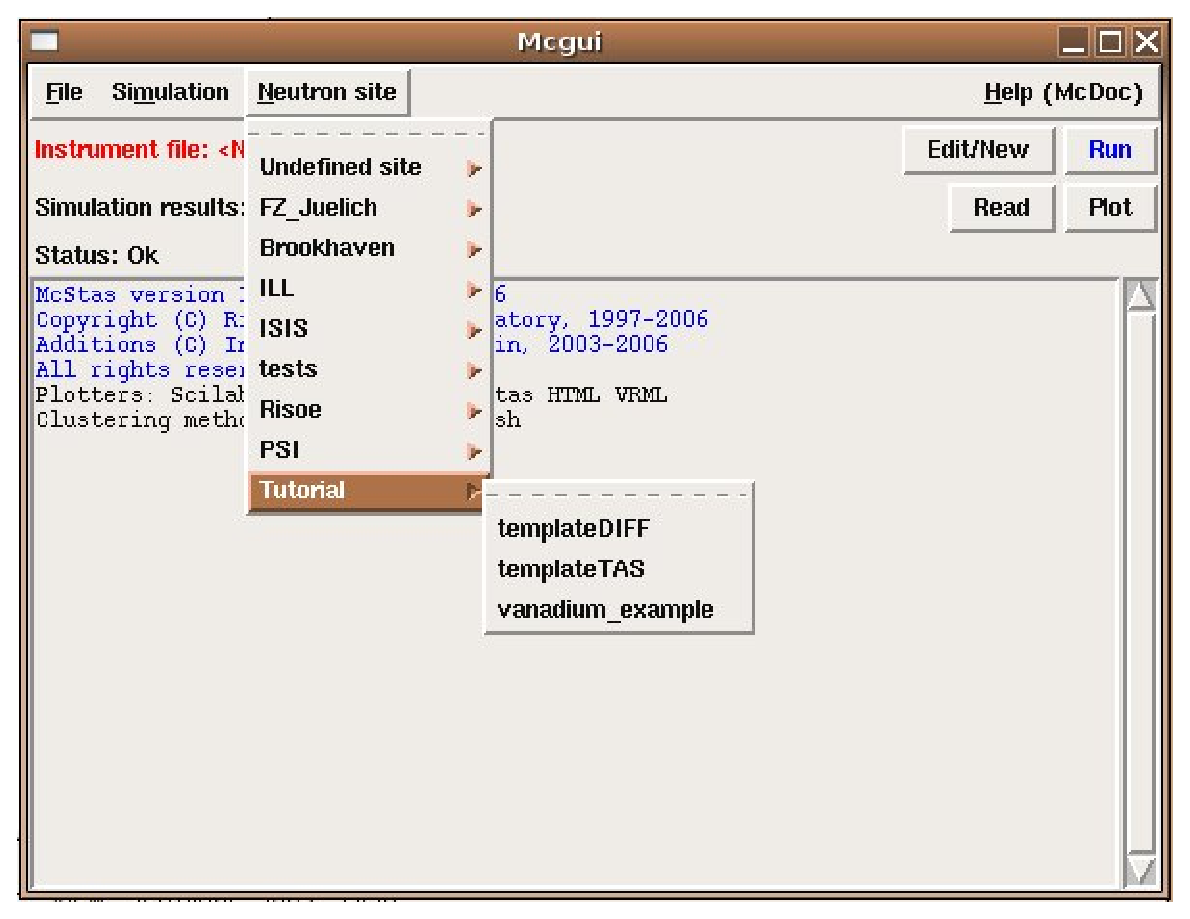
\includegraphics[width=0.55\textwidth]{figures/mcgui.eps}
  \end{center}
\caption{The graphical user interface \texttt{mcgui}.}
\label{fig:mcgui}
\end{figure}

To load an instrument, select ``Tutorial'' from the ``Neutron site''
menu and open the file \verb+vanadium_example+. Next, check that the current plotting backend setting
(select ``Choose backend'' from the ``Simulation'' menu) corresponds
to your system setup. The default setting can be adjusted as explained in Chapter \ref{installing}
\begin{itemize}
\item{by editing
the \verb+tools/perl/mcstas_config.perl+ setup file of your
installation}
\item{by setting the \verb+MCSTAS_FORMAT+ environment
variable.}
\end{itemize} \index{Environment variable!MCSTAS\_FORMAT}
Next, select ``Run simulation'' from the ``Simulation'' menu.
McStas will translate the definition into an executable program and pop
up a dialog window. Type a value for the ``ROT'' parameter ({\em e.g.}
90), check the ``Plot results'' option, and select ``Start''. The
simulation will run, and when it finishes after a while the results will
be plotted in a window. Depending on your chosen plotting backend, the
presented graphics will resemble one of those shown in figure \ref{fig:mcplot_figs}.
\begin{figure}[htb!]
  \begin{center}
    \includegraphics[angle=-90,width=0.49\textwidth]{figures/mcplot_PGPLOT.ps}
    \includegraphics[angle=-90,width=0.49\textwidth]{figures/mcplot_Scilab.eps}
    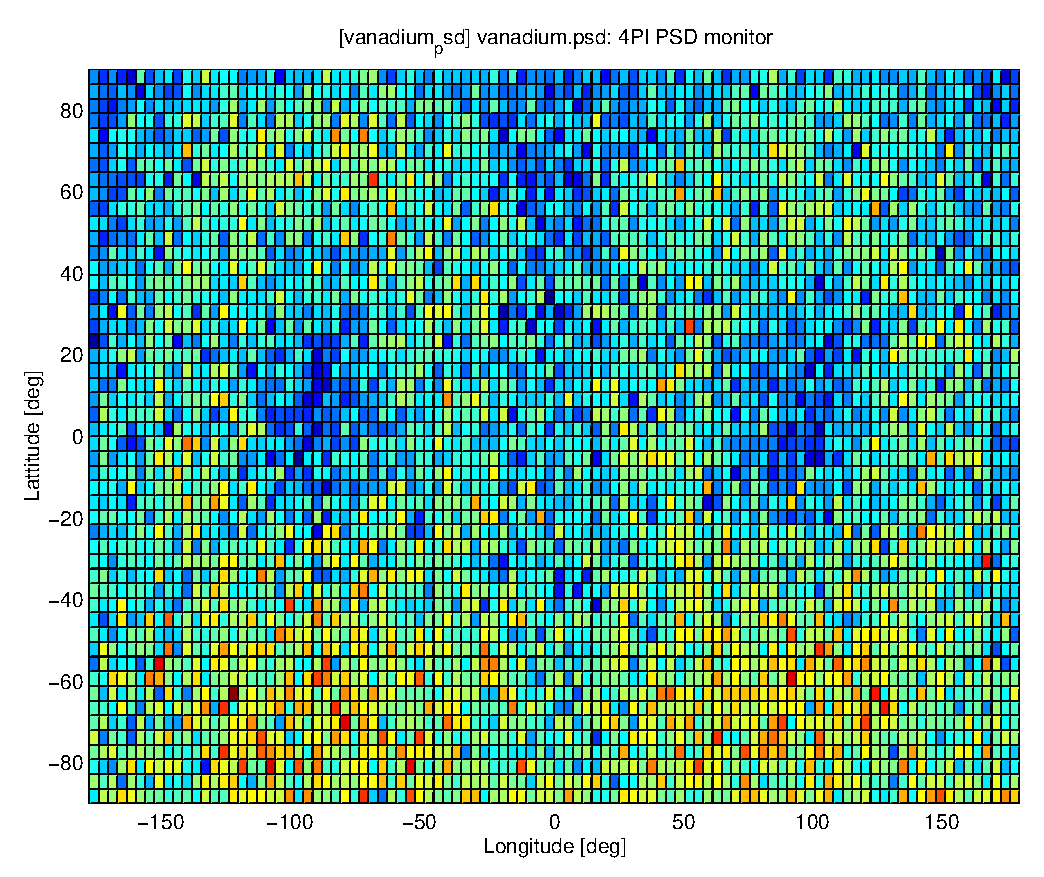
\includegraphics[width=0.49\textwidth]{figures/mcplot_Matlab.eps}
  \end{center}
\caption{Output from \texttt{mcplot} with PGPLOT, Scilab and Matlab backends}
\label{fig:mcplot_figs}
\end{figure}
When using the Scilab or Matlab backends, full 3D view of plots and
different display possibilities are available. Use the attached \MCS\
window menus to control these. Features are quite self
explanatory. For other options, execute \verb+mcplot --help+
(\verb+mcplot.pl --help+ on windows) to get help.


To debug the simulation graphically, repeat the
steps but check the ``Trace'' option instead of the ``Simulate'' option.
A window will pop up showing a sketch of the instrument.
Depending on your
chosen plotting backend, the presented graphics will resemble one of
those shown in figures \ref{fig:mcdisp_PGPLOT}-\ref{fig:mcdisp_Matlab}.
\begin{figure}[htb!]
  \begin{center}
    \includegraphics[width=0.55\textwidth]{figures/mcdisplay_PGPLOT.ps}
  \end{center}
\caption{Output from \texttt{mcdisplay} with PGPLOT backend.
  The left mouse button starts a new neutron, the middle button zooms, and
  the right button resets the zoom. The Q key quits the program.}
\label{fig:mcdisp_PGPLOT}
\end{figure}
\begin{figure}[htb!]
  \begin{center}
    \includegraphics[width=0.55\textwidth]{figures/mcdisplay_Scilab.ps}
    \includegraphics[width=0.25\textwidth]{figures/mcdisplay_Scilab_dialog.ps}
  \end{center}
\caption{Output from \texttt{mcdisplay} with Scilab backend. Display
  can be adjusted using the dialogbox (right).}
\label{fig:mcdisp_Scilab}
\end{figure}
\begin{figure}[htb!]
  \begin{center}
    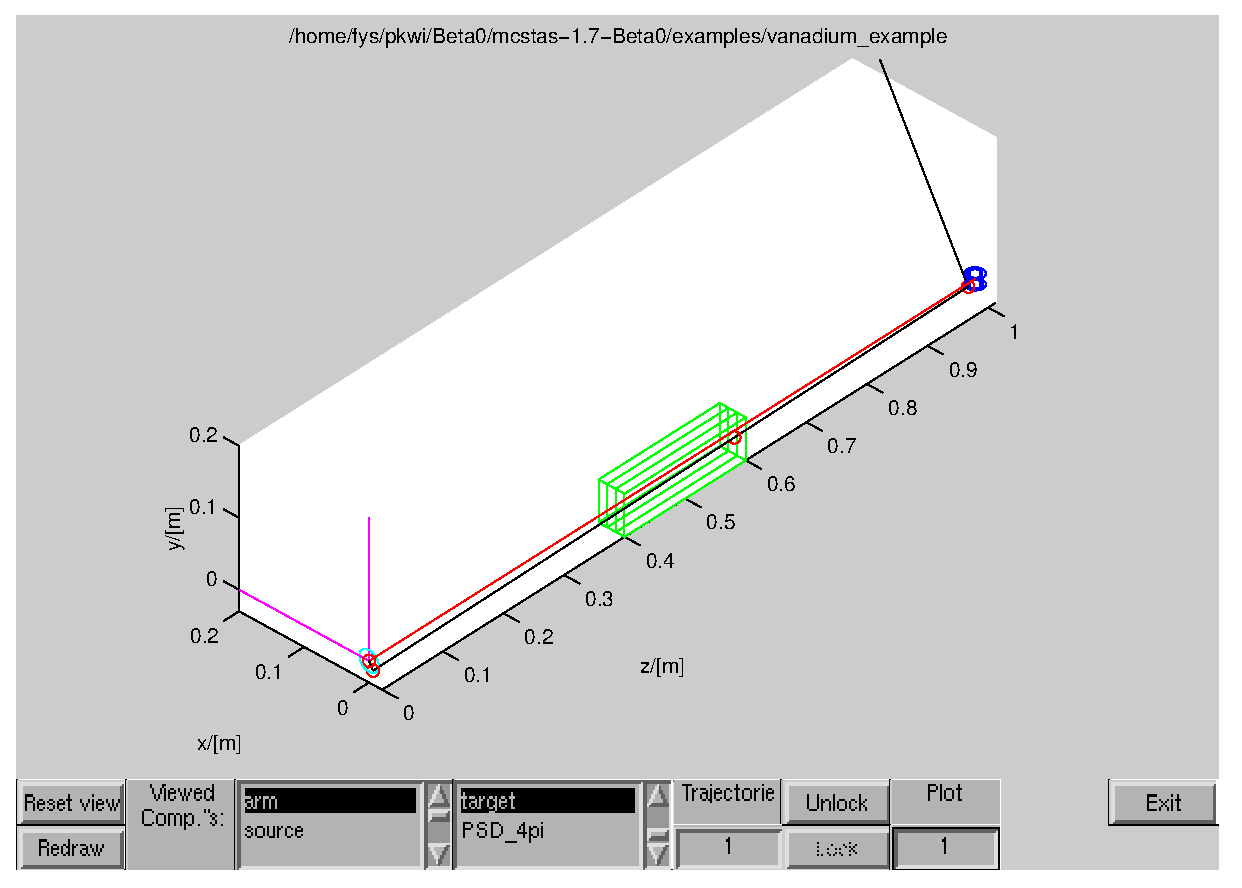
\includegraphics[width=0.55\textwidth]{figures/mcdisplay_Matlab.eps}
  \end{center}
\caption{Output from \texttt{mcdisplay} with Matlab backend. Display
  can be adjusted using the window buttons.}
\label{fig:mcdisp_Matlab}
\end{figure}

For a slightly longer gentle introduction to McStas, see the McStas
tutorial (available from~\cite{mcstas_webpage}), and as of version
\version\ built into the \verb+mcgui+ help menu. For more technical
details, read on from section~\ref{s:running}

\subsection{New releases of \MCS}
Releases of new versions of a software can today be carried out more or less
continuously. However, users do not update their software on a daily basis,
and as a compromise we have adopted the following policy of \MCS\ .

\begin{itemize}
\item A version {\version}.x will possibly contain bug fixes and minor new functionality. A new manual
will, however, not be released and the modifications are documented on the
\MCS\ web-page. The extensions of the forthcoming version {\version}.x are also listed
on the web, and new versions may be released quite frequently when it is requested
by the user community.
\item A version 1.10 will contain important new features and an updated manual. It will typically be released
once or twice a year in connection to for example a \MCS\ workshop.
\end{itemize}

\section{Running the instrument compiler}
\label{s:running}

This section describes how to run the McStas compiler manually. Often,
it will be more convenient to use the front-end program \verb+mcgui+
(section~\ref{s:mcgui}) or \verb+mcrun+ (section~\ref{s:mcrun}). These
front-ends will compile and run the simulations automatically.
\index{Tools!mcgui} \index{Tools!mcrun}

The compiler for the \MCS{} instrument definition
is invoked by typing a command of the form
\begin{verbatim}
    mcstas name.instr
\end{verbatim}
This will read the instrument definition \verb+name.instr+ which is
written in the \MCS\ meta-language. The compiler will translate the
instrument definition into a Monte Carlo simulation program provided in
ANSI-C. The output is by default written to a file in the current
directory with the same name as the instrument file, but with extension
\verb+.c+ rather than \verb+.instr+. This can be overridden using the
\verb+-o+ option as follows:
\begin{verbatim}
    mcstas -o code.c name.instr
\end{verbatim}
which gives the output in the file \verb+code.c+.
A single dash `\verb+-+' may be used for both input and output filename
to represent standard input and standard output, respectively.


\subsection{Code generation options}
\index{Code generation options}

By default, the output files from the \MCS\ compiler are in ANSI-C with
some extensions (currently the only extension is the creation of new
directories, which is not possible in pure ANSI-C). The use of
extensions may be disabled with the \verb+-p+ or \verb+--portable+
option. With this option, the output is strictly ANSI-C compliant, at
the cost of some slight reduction in capabilities.

The \verb+-t+ or \verb+--trace+ option puts special ``trace'' code in
the output. This code makes it possible to get a complete trace of the
path of every neutron through the instrument, as well as the position
and orientation of every component. This option is mainly used with the
\verb+mcdisplay+ front-end as described in section~\ref{s:mcdisplay}.

The code generation options can also be controlled by using preprocessor
macros in the C compiler, without the need to re-run the \MCS\
compiler. If the preprocessor macro \verb+MC_PORTABLE+ is defined, the
same result is obtained as with the \verb+--portable+ option of the
\MCS\ compiler. The effect of the \verb+--trace+ option may be obtained
by defining the \verb+MC_TRACE_ENABLED+ macro. Most Unix-like C
compilers allow preprocessor macros to be defined using the \verb+-D+
option, eg.
\begin{verbatim}
    cc -DMC_TRACE_ENABLED -DMC_PORTABLE ...
\end{verbatim}
Finally, the \verb+--verbose+ option will list the components and libraries beeing
included in the instrument.

\subsection{Specifying the location of files}
\label{s:files}

The \MCS\ compiler needs to be able to find various files during
compilation, some explicitly requested by the user (such as component
definitions and files referenced by \verb+%include+), \index{Keyword!\%include}
and some used internally to generate the simulation executable. \MCS\ looks for these
files in three places: first in the current directory, then in a list of
directories given by the user, and finally in a special \MCS\
directory. Usually, the user will not need to worry about this as \MCS\
will automatically find the required files. But if users build their own
component library in a separate directory or if \MCS\ is installed in an
unusual way, it will be necessary to tell the compiler where to look
for the files.

\index{Library!Components}
The location of the special \MCS\ directory is set when \MCS\ is
compiled. It defaults to \verb+/usr/local/lib/mcstas+ on Unix-like systems and \verb+C:\mcstas\lib+ on Windows systems, but it can be
changed to something else, see section~\ref{s:install} for
details. The location can be overridden by setting the environment
variable \verb+MCSTAS+: \index{Environment variable!MCSTAS}
\begin{verbatim}
    setenv MCSTAS /home/joe/mcstas
\end{verbatim}
for csh/tcsh users, or
\begin{verbatim}
    export MCSTAS=/home/joe/mcstas
\end{verbatim}
for bash/Bourne shell users.
For Windows Users, you should define the \verb+MCSTAS+ from the menu 'Start/Settings/Control Panel/System/Advanced/Environment
Variables' by creating \verb+MCSTAS+ with the value \verb+C:\mcstas\lib+

To make \MCS\ search additional directories for component definitions
and include files, use the \verb+-I+ switch for the \MCS\ compiler:
\begin{verbatim}
    mcstas -I/home/joe/components -I/home/joe/neutron/include name.instr
\end{verbatim}
Multiple \verb+-I+ options can be given, as shown.


\subsection{Embedding the generated simulations in other programs}

By default, \MCS\ will generate a stand-alone C program, which is what
is needed in most cases. However, for advanced usage, such as embedding
the generated simulation in another program or even including two or
more simulations in the same program, a stand-alone program is not
appropriate. For such usage, the \MCS\ compiler provides the following
options:
\begin{itemize}
\item \verb+--no-main+ This option makes \MCS\ omit the \verb+main()+
  function in the generated simulation program. The user must then
  arrange for the function \verb+mcstas_main()+ to be called in some
  way.
\item \verb+--no-runtime+ Normally, the
  generated simulation program contains all the run-time C code necessary for
  declaring functions, variables, etc. used during the simulation.  This
  option makes \MCS\ omit the run-time code from the generated
  simulation program, and the user must then explicitly link with the file
  \verb+mcstas-r.c+ as well as other shared libraries from the \MCS{} distribution.
  \index{Library!Run-time}
\end{itemize}
Users that need these options are encouraged to contact the authors for
further help.


\subsection{Running the C compiler}
\label{s:compile}

After the source code for the simulation program has been generated with
the \MCS\ compiler, it must be compiled with the C compiler to produce
an executable. The generated C code obeys the ANSI-C standard, so it
should be easy to compile it using any ANSI-C (or C++) compiler. \textit{E.g}.\ a
typical Unix-style command would be
\begin{verbatim}
    cc -O -o name.out name.c -lm
\end{verbatim}
The \verb+-O+ option typically enables the optimization phase of the compiler,
which can make quite a difference in speed of \MCS\ generated simulations. The
\verb+-o name.out+ sets the name of the generated executable. The \verb+-lm+
options is needed on many systems to link in the math runtime library (like the
$\cos()$ and $\sin()$ functions). \index{Simulation optimization}

Monte Carlo simulations are computationally intensive, and it is
often desirable to have them run as fast as possible. Some success can
be obtained by adjusting the compiler optimization
options. Here are some example platform and compiler combinations that
have been found to perform well (up-to-date information will be
available on the \MCS\ WWW home page~\cite{mcstas_webpage}):
\begin{itemize}
\item Intel x86 (``PC'') with Linux and GCC, using options \verb+gcc -O3+.
\item Intel x86 with Linux and EGCS (GCC derivate) using
  options \verb+egcc -O6+.
\item Intel x86 with Linux and PGCC (pentium-optimized GCC derivate), using
  options \verb+gcc -O6 -mstack-align-double+.
\item HPPA machines running HPUX with the optional ANSI-C compiler,
  using the options
  \verb|-Aa +Oall -Wl,-a,archive| (the \verb+-Aa+ option is necessary to
  enable the ANSI-C standard).
\item SGI machines running Irix with the options
  \verb|-Ofast -o32 -w|
\end{itemize}
Optimization flags will typically result in a speed improvement by a factor
about 3, but the compilation of the instrument may be 5 times slower.

A warning is in place here: it is tempting to spend far more time
fiddling with compiler options and benchmarking than is actually saved
in computation times. Even worse, compiler optimizations are notoriously
buggy; the options given above for PGCC on Linux and the ANSI-C compiler
for HPUX have been known to generate \emph{incorrect code} in some
compiler versions. \MCS\ actually puts an effort into making the task of the C compiler
easier, by in-lining code and using variables in an efficient way. As a
result, \MCS\ simulations generally run quite fast, often fast enough
that further optimizations are not worthwhile. Also, optimizations are higly
time and memory consuming during compilation, and thus may fail when dealing
with large instrument descriptions (e.g. more that 100 elements). The compilation process is simplified when using components of the library making use of shared libraries (see \verb+SHARE+ keyword in chapter~\ref{s:kernel}). Refer to section \ref{s:optim} for other optimization methods.\index{Optimization}

\section{Running the simulations}
\label{s:run-sim}
\index{Parameters!Instruments}

Once the simulation program has been generated by the \MCS\ compiler
and an executable has been obtained with the C compiler, the simulation
can be run in various ways. The simplest way is to run it directly from the
command line or shell:
\begin{verbatim}
    ./name.out
\end{verbatim}
Note the leading dot, which is needed if the current directory is not in
the path searched by the shell. When used in this way, the simulation
will prompt for the values of any instrument parameters such as motor
positions, and then run the simulation. Default instrument parameter values (see section~\ref{s:instrdefs}), if any, will be indicated and entered when hitting the \verb+Return+ key.\index{Parameters!Optional, default value}
This way of running \MCS\ will only give data for one spectrometer
setting which is normally sufficient {\em e.g.} for a time-of-flight
spectrometer, but not for a triple-axis spectrometer where a scan over
various spectrometer settings is required.
Often the simulation will be run using one of several
available front-ends, as described in the next section. These front-ends
help manage output from the potentially many detectors in the
instruments, as well as running the simulation for each data point in
a scan.

The generated simulations accept a number of options and arguments. The
full list can be obtained using the \verb+--help+ option:
\begin{verbatim}
    ./name.out --help
\end{verbatim}
The values of instrument parameters may be specified as arguments using
the syntax \textit{name}\verb+=+\textit{val}. For example
\begin{verbatim}
    ./vanadium_example.out ROT=90
\end{verbatim}
\index{Parameters!Instruments}
The number of neutron histories to simulate may be set using the
\verb+--ncount+ or \verb+-n+ option, for example
\verb+--ncount=2e5+. The initial seed for the random number generator is
by default chosen based on the current time so that it is different for
each run. However, for debugging purposes it is sometimes convenient to
use the same seed for several runs, so that the same sequence of random
numbers is used each time. To achieve this, the random seed may be set
using the \verb+--seed+ or \verb+-s+ option.

By default, \MCS\ simulations write their results into several data files in the
current directory, overwriting any previous files stored there. The
\verb+--dir=+\textit{dir} or \verb+-d+\textit{dir} option causes the files to be
placed instead in a newly created directory \textit{dir} (to prevent overwriting
previous results an error message is given if the directory already exists).
Alternatively, all output may be written to a single file \textit{file} using
the \verb+--file=+\textit{file} or \verb+-f+\textit{file} option (which should
probably be avoided when saving in binary format, see below).

The complete list of options
and arguments accepted by \MCS\ simulations appears in
table~\ref{f:simoptions}.

\subsection{Choosing an output data file format}

Data files contain header lines with information about the
simulation from which they originate. In case the data must be analyzed
with programs that cannot read files with such headers, they may be
turned off using the \verb+--data-only+ or \verb+-a+ option.
\index{Data format}

The format of the output files from \MCS\ simulations is described in
more detail in section~\ref{s:analyze}. It may be chosen either with \verb+--format=FORMAT+ for each simulation or globally by setting the MCSTAS\_FORMAT environment variable. \index{Environment variable!MCSTAS\_FORMAT}
The available format list is obtained using the \verb+name.out --help+ option, and shown in table~\ref{t:formatoptions}.
\MCS\ can presently generate many formats, including the original \MCS /PGPLOT and the new Scilab and Matlab formats. All formats, except the \MCS /PGPLOT, may eventually support binary files, which are much smaller and faster to import, but are platform dependent. The simulation data file extensions are appended automatically, depending on the format, if the file names do not contain any. Binary files are particularly recommanded for the IDL format (e.g. \verb+--format=IDL_binary+), and the Matlab and Scilab format when handling large detectors (e.g. more than 50x50 bins). For example:
\begin{verbatim}
    ./vanadium_example.out ROT=90 --format="Scilab_binary"
\end{verbatim}
or more generally (for bash/Bourne shell users)
\begin{verbatim}
    export MCSTAS_FORMAT="Matlab"
    ./vanadium_example.out ROT=90
\end{verbatim}

It is also possible to create \textit{Vitess} and \textit{Tripoli4} neutron event files using the \verb+Vitess_input+/\verb+Vitess_output+ and \verb+Tripoli_input+/\verb+Tripoli_output+ components respectively. \index{Vitess} \index{Tripoli}

Additionally, adding the \texttt{raw} keyword to the FORMAT will produce raw $[N, p, p^2]$ data sets instead of $[N, p, \sigma]$ (see Section \ref{s:staterror}). The former representation is fully additive, and thus enables to add results from separate simulations (e.g. when using a computer Grid).

\subsection{Basic import and plot of results}
\label{s:run-format}
The previous example will result in a \verb+mcstas.m+ file, that may be read directly from Matlab (using the {\it sim file} function)
\begin{verbatim}
    matlab> s=mcstas;
    matlab> s=mcstas('plot')
\end{verbatim} \index{Tools!Matlab}
The first line returns the simulation data as a single structure variable, whereas the second one will additionally plot each detector separately.
This also equivalently stands for Scilab (using the \verb+get_+{\it sim file} function, the 'exec' call is required in order to compile the code)
\begin{verbatim}
    scilab> exec('mcstas.sci', -1); s=get_mcstas();
    scilab> exec('mcstas.sci', -1); s=get_mcstas('plot')
\end{verbatim} \index{Tools!Scilab}
and for IDL
\begin{verbatim}
    idl> s=mcstas()
    idl> s=mcstas(/plot)
\end{verbatim} \index{Tools!IDL}
See section~\ref{s:mcplot} for an other way of plotting simulation results using the \verb+mcplot+ front-end. \index{Tools!mcplot}

When choosing the HTML format, the simulation results are save as a web page, whereas the monitor data files are saved as VRML files, displayed within the web page.

\begin{table}
  \begin{center}
    {\let\my=\\
    \begin{tabular}{|p{0.24\textwidth}|p{0.7\textwidth}|}
      \hline
      \texttt{-s {\it seed}} \my \texttt{--seed={\it seed}}
        & Set the initial seed for the random number generator. This may be
        useful for testing to make each run use the same random number
      sequence. \\
      \hline
      \texttt{-n {\it count}} \my \texttt{--ncount={\it count}}
        & Set the number of neutron histories to simulate. The default
      is 1,000,000. \\
      \hline
      \texttt{-d {\it dir}} \my \texttt{--dir={\it dir}}
        & Create a new directory {\it dir\/} and put all data files in
      that directory. \\
      \hline
      \texttt{-f {\it file}} \my \texttt{--file={\it file}}
        & Write all data into a single file {\it file}. Avoid when using binary formats. \\
      \hline
      \texttt{-a} \my \texttt{--data-only}
        & Do not put any headers in the data files. \\
      \hline
      \texttt{-h} \my \texttt{--help}
        & Show a short help message with the options accepted, available formats
        and the names of the parameters of the instrument. \\
      \hline
      \texttt{-i} \my \texttt{--info}
        & Show extensive information on the simulation and the
      instrument definition it was generated from. \\
      \hline
      \texttt{-t} \my \texttt{--trace}
        & This option makes the simulation output the state of every
      neutron as it passes through every component. Requires that the
      \texttt{-t} (or \texttt{--trace}) option is also given to the
      \MCS\ compiler when the simulation is generated. \\
      \hline
      \texttt{--no-output-files}
        & This option disables the writing of data files (output to the
      terminal, such as detector intensities, will still be written). \\
      \hline
      \texttt{-g} \my \texttt{--gravitation}
        & This option toggles the gravitation (approximation) handling for the whole neutron propagation within the instrument. May produce wrong results depending on the components.\\
      \hline
      \texttt{--format={\it FORMAT}}
        & This option sets the file format for result simulation and data files. \\
      \hline
      \texttt{--format\_data={\it FORMAT}}
        & This option sets the file format for result data files from monitors. This enables to have simulation files in one format (e.g. HTML), and monitor files in an other format (e.g. VRML).\\
      \hline
      \texttt{{\it param}{\texttt =}{\it value}}
        & Set the value of an instrument parameter, rather than having
        to prompt for each one. \\
      \hline
    \end{tabular}
    \caption{Options accepted by \MCS\ simulations}
    \label{f:simoptions}
    }
  \end{center}
\end{table}

\begin{table}
  \begin{center}
    {\let\my=\\
    \begin{tabular}{|p{0.24\textwidth}|c|p{0.7\textwidth}|}
      \hline
      \texttt{\MCS} \my \texttt{PGPLOT} & .sim & Original format for PGPLOT plotter (may be used with -f and -d options) \\
      \texttt{Scilab} & .sci & Scilab format (may be used with -f and -d options) \\
      \texttt{Scilab\_binary} & & Scilab format with external binary files (may be used with -d option). Also toggles -a option. \\
      \texttt{Matlab} & .m & Matlab format (may be used with -f and -d options) \\
      \texttt{Matlab\_binary} & & Matlab format with external binary files (may be used with -d option). Also toggles -a option. \\
      \texttt{Octave} & .m & Octave format (may be used with -f and -d options) \\
      \texttt{Octave\_binary} & & Octave format with external binary files (may be used with -d option). Also toggles -a option. \\
      \texttt{IDL} & .pro & IDL format. {\em Must} be used with -f option. \\
      \texttt{IDL\_binary} & & IDL format with external binary files (may be used with -d option). Also toggles -a option. \\
      \texttt{XML} & .xml & XML/NeXus format (may be used with -f and -d options). \\
      \texttt{HTML} & .html & HTML format (generates a web page, may be used with -f and -d options). Data files are saved as VRML objects. \\
      \texttt{VRML} & .wrl & Virtual Reality file format for data files. Simulation files are not saved properly, and the HTML format should be used preferably. \\
      {\it Tripoli} &  & Tripoli 4 neutron events file format. Use \verb+Virtual_tripoli4_input+/\verb+Virtual_tripoli4_output+ components. \\
      {\it Vitess} &  & Vitess neutron events file format. Use \verb+Vitess_input+/\verb+Vitess_output+ components. \\
      {\it McStas events} & & McStas event files in text or binary format. Use \verb+Virtual_input+/\verb+Virtual_output+ components. \\
      \hline
    \end{tabular}
    \caption{Available formats supported by \MCS\ simulations.}
    \label{t:formatoptions}
    }
  \end{center}
\end{table}

\subsection{Interacting with a running simulation}
\index{Signal handler|textbf}

Once the simulation has started, it is possible, under Unix, Linux and Mac OS X systems, to interact with the on-going simulation.

\MCS\ attaches a signal handler to the simulation process. In order to send a signal to the process, the process-id {\it pid} must be known. Users may look at their running processes with the Unix 'ps' command, or alternatively process managers like 'top' and 'gtop'.
If a {\it file.out} simulation obtained from \MCS\ is running, the process status command should output a line ressembling
\begin{quote}
  \verb|<user>| {\it 13277} \verb|7140 99 23:52 pts/2    00:00:13 | {\it file.out}\\
\end{quote}
where \verb+user+ is your loggin name. The {\it pid} is there '13277'.

Once known, it is possible to send one of the signals listed in table~\ref{t:signals} using the 'kill' unix command (or the functionalities of your process manager), e.g.
\begin{verbatim}
    kill -USR2 13277
\end{verbatim}
This will result in a message showing status (here 33 \% achieved), as well as the position in the instrument of the current neutron.
\begin{verbatim}
# McStas: [pid 13277] Signal 12 detected SIGUSR2 (Save simulation)
# Simulation: file (file.instr)
# Breakpoint: MyDetector (Trace) 33.37 % (  333654.0/ 1000000.0)
# Date      : Wed May  7 00:00:52 2003
# McStas: Saving data and resume simulation (continue)
\end{verbatim}
followed by the list of detector outputs (integrated counts and files). Finally, sending a \verb+kill 13277+ (which is equivalent to \verb+kill -TERM 13277+) will end the simulation before the initial 'ncount' preset.

A typical usage example would be, for instance, to save data during a
simulation, plot or analyze it, and decide to interupt the simulation
earlier if the desired statistics has been achieved. This may be done automatically using the \verb+Progress_bar+ component.

Whenever simulation data is generated before end (or the simulation is interupted), the 'ratio' field of the monitored data will provide the level of achievement of the computation (for instance '3.33e+05/1e+06'). Intensities are then usually to be scaled accordingly.

Additionally, any system error will result in similar messages, giving indication about the occurence of the error (in which component ? in which section ?). Whenever possible, the simulation will {\em try} to save the data before ending. Most errors appear when writing a new component, in the \texttt{INITIALIZE}, \texttt{TRACE} or \texttt{FINALLY} sections. Memory errors usually show up when C pointers have not been allocated/unallocated before usage, whereas mathematical errors are set when, for instance, dividing per zero.

\begin{table}
  \begin{center}
    {\let\my=\\
    \begin{tabular}{|p{0.24\textwidth}|p{0.7\textwidth}|}
      \hline
      \texttt{USR1} & Request informations (status)  \\
      \texttt{USR2, HUP} & Request informations and performs an intermediate saving of all monitors (status and save). This triggers the execution of all \texttt{SAVE} sections (see chapter~\ref{s:kernel}).  \\
      \texttt{INT, TERM} & Save and exit before end (status)  \\
      \hline
    \end{tabular}
    \caption{Signals supported by \MCS\ simulations.}
    \label{t:signals}
    }
  \end{center}
\end{table}

\subsection{Optimizing a simulation}
\index{Optimization|textbf}
\label{s:optim}
There are various other ways to speed-up a simulation
\begin{itemize}
\item Optimize the compilation of the instrument, as explained in section~\ref{s:compile}.
\item Execute the simulation in parallel on a computer grid or a cluster (with MPI) as explained in section~\ref{s:run-mpi}.
\item Divide simulation into parts using a file for saving or generating neutron
      events. This way, a guide may be simulated only once, saving the neutron events
      getting out from it as a file, which is being read quickly by the second simulation
      part. Use the Virtual\_input and Virtual\_output components for this technique.
\item Use source optimizers like the components Source\_adapt or
      Source\_Optimizer. Such component may sometimes not be very efficient, when no
      neutron importance sampling can be achieved, or may even sometimes alter the
      simulation results. Be careful and always check results with a non-optimized
      computation.
\item Complex components usually take into account additional small effects in a simulation,
      but are much longer to execute. Thus, simple components should be prefered
      whenever possible, at least to start with.
\end{itemize}

Additionally, the user may wish to optimize the parameters of a simulation (e.g. find the optimal curvature of a monochromator, or the best geometry of a given component).
The user should write a function script or a program that
\begin{itemize}
\item inputs the simulation parameters, which are usually numerical values such as $TT$ in the \verb+prisma2+ instrument from the \verb+examples+ directory of the package.
\item builds a command line from these parameters.
\item execute that command, and waits until the end of the computation.
\item reads the relevant data from the monitors.
\item outputs a simulation quality measurement from this data, usually the integrated counts or some peak width.
\end{itemize}

For instance, for the \verb+prisma2+ instrument we could write a function for Matlab (see section~\ref{s:analyze} for details about the Matlab data format) in order to study the effects of the $TT$ parameter:
\begin{verbatim}
  function y = instr_value(p)
    TT = p(1);     % p may be a vector/matrix containing many parameters
    syscmd = [ 'mcrun prisma2.instr -n1e5 TT=' num2str(TT) ...
               ' PHA=22 PHA1=-3 PHA2=-2 PHA3=-1 PHA4=0 PHA5=1' ...
               ' PHA6=2 PHA7=3 TTA=44 --format="Matlab binary"' ];
    system(syscmd); path(path) % execute simulation, and rehash files
    s = mcstas;     % get the simulation data, and the monitor data
    s = s.prisma2.m_mcstas.detector.prisma2_tof.signal;
    eval(s);        % we could also use the 'statistics' field
    y = -Mean;      % 'value' of the simulation
\end{verbatim}

Then a numerical optimization should be available, such as those provided with Matlab, Scilab, IDL, and Perl-PDL high level languages. In this example, we may wish to maximize the \verb+instr_value+ function value. The \verb+fminsearch+ function of Matlab is a minimization method (that's why we have a minus sign for $y$ value), and:
\begin{verbatim}
    matlab> TT = fminsearch('instr_value', -25)
\end{verbatim}
will determine the best value of TT, starting from -25 estimate, in order to minimize function \verb+instr_value+, and thus maximize the mean detector counts.

The choice of the optimization routine, of the simulation quality value to optimize
and the initial parameter guess all may have a large influence on the results.
Be cautious and wise when interpreting the optimal guess.

\section{Using computer Grids and Clusters}
\label{s:run-mpi}
\index{Parallel computing|textbf}
\index{MPI|textbf}\index{Grid computing|textbf}\index{mcstas-hosts}

Parallelizing a computation is possible when dependencies between
  each computation are not too strong. The situation of \MCS\ is
  ideal since each neutron can be simulated without interfering with
  other simulated neutrons. Therefore each neutron can be simulated
  independently on a set of computer.

\MCS\ provides two methods in order to distribute computations on many computers.
\begin{itemize}
\item when scanning instrument parameters (using \texttt{mcrun --multi -N}),
  it is possible to distribute each scan step on a list of computers.
\item when using an homogeneous computer cluster, each simulation (including scan
  steps) may be computed in parallel using MPI (using \texttt{mcrun --mpi=Nb\_Nodes}).
\end{itemize}

\subsection{Distribute mcrun scans (grid)}
  This is an experimental option to
  distribute scan steps on a set of machines using \emph{ssh}
  connexions. To use this option you will need
  \begin{itemize}
  \item{A set of unix machines of the same architecture (binary compatible). All
      machines should have the same \MCS\ distribution installed.}
  \item{ \texttt{ssh} access from the master node (where McStas is
      installed) to the slaves through e.g. DSA keys \emph{without} a
      password. These keys should be generated using the command
      \texttt{ssh-keygen}. Run \emph{e.g.} \texttt{ssh-keygen -t dsa} on
      master node, enter no passphrase and add resulting
      \texttt{.ssh/id\_dsa.pub} to \texttt{.ssh/authorized\_keys}
      on all the slave nodes.}
  \item{The machine names listed in the file \texttt{.mcstas-hosts} in
      your home directory or in the \texttt{MCSTAS/tools/perl/mcstas-hosts} on
      the master node, one node per line. The \verb'--machines=<file>' option
      enables to specify the hosts file to use.}
  \item{Execute \texttt{mcrun} as normally, appending \texttt{--multi} or
      \texttt{-M} will divide the $N$ scanpoints across the machines in
      \texttt{.mcstas-hosts $+$ localhost}.}
  \end{itemize}
  Each of the scan steps is executed on distant machines, sending the executable
  with \emph{scp}, executing single simulations, and then retrieving individual
  scan steps on the master machine.
  {\bf Warning:} This option is considered \emph{experimental} - i.e.,
  you are welcome to use it, but be ready for trouble. Note also that
  this is a unix only option in \texttt{mcgui} and \texttt{mcrun}, it
  {\bf does not} work on windows.

\subsection{Parallel computing (MPI)}

When computing $N$ neutrons with
$p$ computers, each computer will simulate $\frac{N}{p}$
neutrons. As a result there will be $p \cdot \frac{N}{p} \leq N$
neutrons simulated. As a result, \MCS\ generates two kinds of data sets:
\begin{itemize}
\item intensity measurements, internally represented by three
  values $(p_0, p_1, p_2)$ where $p_0$, $p_1$, $p_2$ are
  additive. Therefore the final value of $p_0$ is the sum of all
  local value of  $p_0$ computed on each node. The same rule applies
  for $p_1$ and $p_2$. The evaluation of the intensity errors $\sigma$
  is performed using the final $p_0$, $p_1$, and $p_2$ arrays (see Section \ref{s:staterror}).
\item event lists: the merge of events is done by concatenation
\end{itemize}
The MPI support requires to have MPICH, or alternatively LAM-MPI, installed on a set of nodes.
This usually also requires to setup properly the \texttt{ssh} connections and keys.

\subsubsection{MPI Basic usage}

To enable parallel computation, compile McStas output C-source file
with \verb'mpicc' with the flag \verb'-DUSE_MPI' and run it using the
wrapper of your MPI implementation (\verb'mpirun' for mpich or lammpi) :
\begin{verbatim}
  # generate a C-source file [sim.c]
  mcstas sim.instr

  # generate an executable with MPI support [sim.mpi]
  mpicc -DUSE_MPI -o sim.mpi sim.c

  # execute with parallel processing over <N> computers
  # here you have to list the computers you want to use
  # in a file [machines.list] (using mpich implementation)
  # (refer to MPI documentation for a complete description)
  mpirun -machinefile machines.list -n <N> \
         ./sim.mpi <instrument parameters>
  ...
\end{verbatim}

If you don't want to spread the simulation, run it as usual :
\begin{verbatim}
  ./sim.mpi <instrument parameters>
\end{verbatim}

If you want to disable MPI support (for example if you do not have MPI
installed), just compile the C-source file generated by \verb'mcstas'
  without \verb'mpicc' and without the \verb'-DUSE_MPI' flag :
\begin{verbatim}
  # generate a C-source file [sim.c]
  mcstas sim.instr

  # generate an executable without MPI support [sim.no_mpi]
  cc -o sim.no_mpi sim.c

  # execute on a single computer
  ./sim.no_mpi <instrument parameters>
  ...
\end{verbatim}

\subsection{McRun script with MPI support}

The \verb'mcrun' script has been adapted to use MPICH implementation
of MPI. Two new options have been added:
\begin{itemize}
\item \verb'--mpi=<number>': tells \verb'mcrun' to use MPI, and to
  spread the simulation over \verb'<number>' nodes
\item \verb'--machines=<file>': defines a text file where the
  nodes which are to be used for parallel computation are listed; by
  default, \verb'mcrun' will look at \verb'$HOME/.mcstas-hosts' and
  \verb'MCSTAS/tools/perl/mcstas-hosts'.
\end{itemize}

Suppose you have four machines named \verb'node1' to \verb'node4'.
A typical machine list file, \verb'machines.list' looks like :
\begin{verbatim}
node1
node2
node3
node4
\end{verbatim}

You can then spread a simulation \verb'sim.instr' using \verb'mcrun' :
\begin{verbatim}
  mcrun -c --mpi=4 --machines=machines.list \
        sim.instr <instrument parameters>
\end{verbatim}

\begin{paragraph}{Warning:} when using \verb'mcrun' with MPI, be sure
  to recompile your simulation with MPI support (see \verb'-c' flag of
  \verb'mcrun'): a simulation compiled without MPI support cannot be
  used with MPI, whereas a simulation compiled with MPI support can be
  used without MPI.
\end{paragraph}

\subsection{McStas/MPI Performance}

Theorically, a computation which lasts $T$ seconds on a single computer,
should lasts at least $\frac{T}{p}$ seconds when it is distributed
over $p$ computers. There is a eventually overhead due to the split
and merge operations.
\begin{itemize}
\item the split is immediate: constant time cost ${\cal O}(1)$
\item the merge is at worst linear against the number of computers:
  \begin{itemize}
  \item linear time cost~: ${\cal O}(p)$ when saving an event list
  \item logarithmic time cost: ${\cal O}(\log{p})$ when not saving an
  event list
  \end{itemize}
\end{itemize}

Here is a table showing some comparison between MPI and no-MPI
simulations. The cluster is built with 2 bi-xeon 2GHz, resulting in 4
nodes.
\begin{center}
  \begin{tabular}{|c|c|l|}
    \hline
    \# nodes & duration (seconds) & notes \\
    \hline
    1 & 622 & without MPI support \\
    1 & 630 & with MPI support, run without MPI \\
    1 & 620 & with MPI support, run with MPI \\
    \hline
    2 & 316 & \\
    3 & 210 & \\
    4 & 158 & \\
    \hline
  \end{tabular}
\end{center}

These benchmarks are consistent~: there is a really small overhead
when computing using MPI. This overhead comes from the spread and the
fusion of the computations. For instance, spreading a computation
implies either an \verb'rsh' or and \verb'ssh' session to be opened on
every node.

\subsection{McStas/MPI Bugs and limitations}

\begin{itemize}
\item when simulating $N$ neutrons with $p$ machines, the effective
  number of neutrons simulated is $p \cdot \frac{N}{p}$
\item signals are \emph{not} supported while simulating with MPI (since
  asynchrone events cannot be easily transmitted to all nodes). Anyway,
  depending on the MPI implementation, you may force all nodes to synchronize
  and save data using the HUP signal (\verb'kill -HUP mcstasPID').
\item some header of output files might contain minor errors
\item the computation split doesn't take into account the speed or the
  load of nodes: the overall time of a distributed computation is
  forced by the slowest node; the ``cluster'' is supposed to be
  homogeneous
\item forcing the random seed while spreading the computation doesn't
  work since every node will use identical seeds and will then
  generate identical pseudo-random values
\item MPI must be correctly configured: if using \verb'ssh', you
  have to set ssh keys so as not to have to enter any password; if
  using \verb'rsh', you have to set a \verb'.rhosts' file
\end{itemize}

\section{Using simulation front-ends}
\label{s:frontends}

\MCS\ includes a number of front-end programs that extend the
functionality of the simulations. A front-end program is an interface
between the user and the simulations, running the simulations and
presenting the output in various ways to the user.

The list of available \MCS\ front-end programs may be obtained from the \verb+mcdoc --tools+ command:
\begin{verbatim}
    McStas Tools
       mcstas        Main instrument compiler
       mcrun         Instrument maker and execution utility
       mcgui         Graphical User Interface instrument builder
       mcdoc         Component library documentation generator/viewer
       mcplot        Simulation result viewer
       mcdisplay     Instrument geometry viewer
       mcresplot     Instrument resolution function viewer
       mcstas2vitess McStas to Vitess component translation utility
       mcconvert     Matlab <-> Scilab script conversion tool
    When used with the -h flag, all tools display a specific help.
    SEE ALSO: mcstas, mcdoc, mcplot, mcrun, mcgui, mcresplot, mcstas2vitess
    DOC:      Please visit http://neutron.risoe.dk/mcstas/
\end{verbatim}
An extended set of front-end programs is planned for future versions of
\MCS, including a NeXus data format option~\cite{nexus_webpage}.


\subsection{The graphical user interface (mcgui)}
\label{s:mcgui}
\index{Tools!mcgui|textbf}

The front-end \verb+mcgui+ provides a graphical user interface that
interfaces the various parts of the McStas package. It is started using
simply the command
\begin{verbatim}
    mcgui
\end{verbatim}
The mcgui (mcgui.pl on Windows) program may optionally be given the name of an instrument file.

When the front-end is started, a main window is opened (se figure \ref{fig:mcgui}). This window
displays the output from compiling and running simulations, and also
contains a few menus and buttons. The main purpose of the front-end is
to edit and compile instrument definitions, run the simulations, and
visualize the results.

\subsubsection{The menus}

The ``File'' menu has the following features:
\begin{description}
\item[Open instrument] selects the name of an instrument file to be used.
\item[Edit current] opens a simple editor window for editing the
  current instrument definition. This function is also available from
  the ``Edit'' button to the right of the name of the instrument definition in
  the main window.
\item[Spawn editor] This starts the editor defined in the environment
  variable \verb+VISUAL+ or \verb+EDITOR+ on the current instrument
  file. It is also possible to start an external editor manually; in any
  case \verb+mcgui+ will recompile instrument definitions as necessary based on
  the modification dates of the files on the disk.
  \index{Environment variable!EDITOR}
\item[Compile instrument] forces a recompile of the instrument
  definition, regardless of file dates. This is for example useful to
  pick up changes in component definitions, which the front-end will not
  notice automatically. See section~\ref{s:install} for how to override
  default C compiler options.
\item[Clear output] erases all text in the window showing output of
  compilations and simulations.
\item[Quit] exits the graphical user interface front-end.
\end{description}

\noindent The ``Simulation'' menu has the following features:
\begin{description}
\item[Read old simulation] prompts for the name of a file
  from a previous run of a McStas simulation (usually called
  \verb+mcstas.sim+). The file will be read and any detector data
  plotted using the \verb+mcplot+ front-end. The parameters used in the
  simulation will also be made the defaults for the next simulation
  run. This function is also available using the ``Read'' button to the
  right of the name of the current simulation data.
\item[Run simulation] opens the run dialog window, explained
  further below.
\item[Plot results] plots (using \verb+mcplot+) the results of the
  last simulation run or loaded.
\item[Configuration options] selection of plotting backend
  (PGPLOT/Matlab/Scilab). Opens the choose backend dialog shown in
  figure~\ref{fig:mcgui-choose}. All formats are chosen as full text, but a 'Use binary files' option is possible. Additionally, the editor to use to list instrument descriptions can be chosen. The HTML/VRML data files save results as a web-page document requiring a VRML viewer to display the data files as a 3D surface.
\end{description}

\noindent The ``Neutron Site'' menu contains a list of template/example instruments as found in the \MCS\ library, sorted by neutron site. When selecting one of these, a local copy of the instrument description is transfered to the active directory (so that users have modification rights). One may then view its source (Edit) and use it directly for simulations/trace (3D View).
 \begin{figure}[htb!]
  \begin{center}
    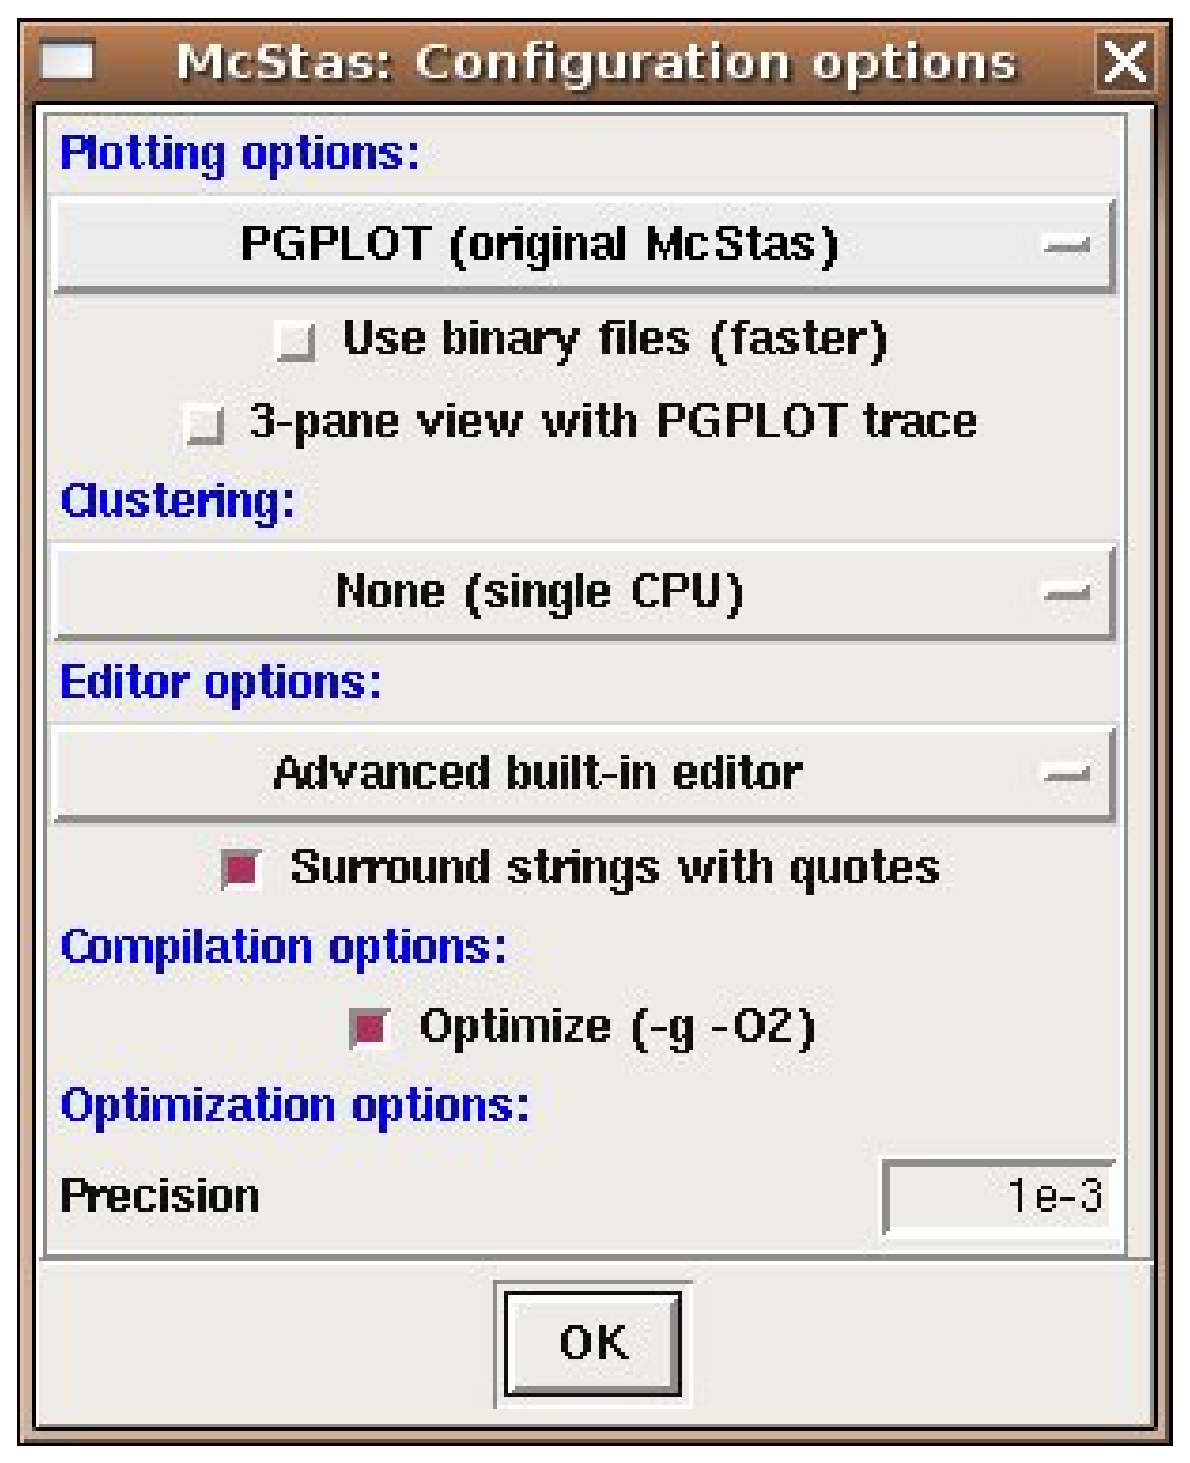
\includegraphics[width=0.3\textwidth]{figures/choose_backend.eps}
  \end{center}
\caption{The choose backend dialog in \texttt{mcgui}.}
\label{fig:mcgui-choose}
\end{figure}

The ``Help'' menu has the following features, through use of
\verb+mcdoc+ and a web browser. To customize the used web browser, set
the \verb+BROWSER+ environment variable. If \verb+BROWSER+ is not set,
\verb+mcgui+ uses \verb+netscape+ on Unix and the default browser on
Windows.
\begin{description}
\item[\MCS\ User manual] calls \verb+mcdoc --manual+, brings up the local
  pdf version of this manual, using a web browser.
\item[\MCS\ Component manual] calls \verb+mcdoc --comp+, brings up the local
  pdf version of the component manual, using a web browser.
\item[Component library index] displays the component documentation using
  the component \verb+index.html+ index file.
\item[\MCS\ web page] calls \verb+mcdoc --web+, brings up the \MCS\
  website in a web browser.
\item[Tutorial] opens the \MCS\ tutorial for a quick start.
\item[Current instrument info] generates a description web-page of the current edited instrument.
\item[Test \MCS\ installtion] launches a self test procedure to check that the \MCS\ package is installed properly, generates accurate results, and may use the plotter to display the results.
\item[Generate component index] (re-)generates locally the component \verb+index.html+.

\end{description}

\subsubsection{The run dialog}

\begin{figure}[htb!]
  \begin{center}
    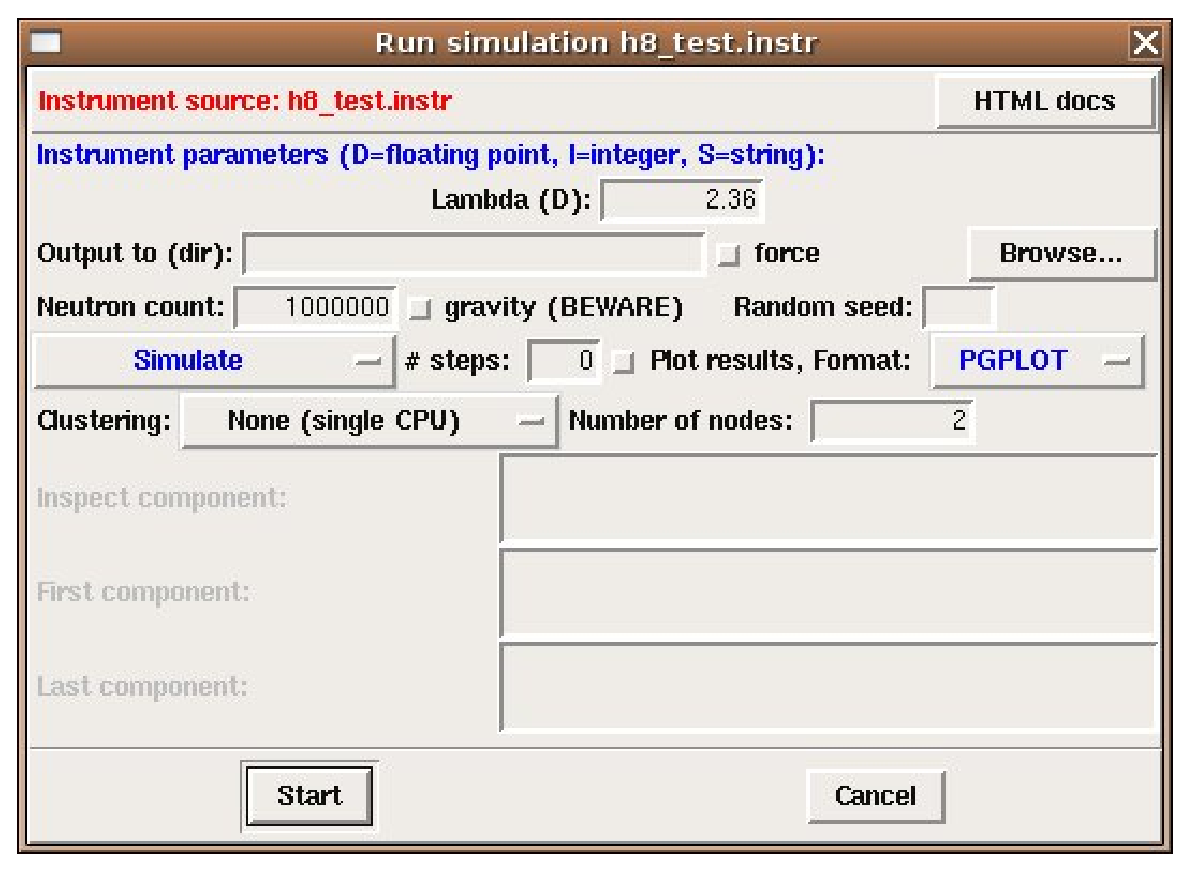
\includegraphics[width=0.45\textwidth]{figures/mcgui-run.eps}
  \end{center}
\caption{The run dialog in \texttt{mcgui}.}
\label{fig:mcgui-run}
\end{figure}
%
The run dialog is used to run simulations. It allows the entry of
instrument parameters as well as the specifications of options for
running the simulation (see section~\ref{s:run-sim} for details). It
also allows to run the \verb+mcdisplay+ (section~\ref{s:mcdisplay}) and
\verb+mcplot+ (section~\ref{s:mcplot}) front-ends together with the
simulation.

The meaning of the different fields is as follows:
\begin{description}
\item[Instrument parameters] allows the setting of the values for
  the input parameters of the instrument. The type of each instrument
  parameter is given in parenthesis after each name. Floating point
  numbers are denoted by (D) (for the C type ``\verb+double+''), (I)
  denotes integer parameters, and (S) denotes strings. For parameter scans, enter the minimum and maximum values to scan, separated by a coma, e.g. \verb+1,10+ and do not forget to set the {\bf \# Scanpoints} to more than 1.
\item[Output to] allows the entry of a directory to store the
  resulting data files in (like the \verb+--dir+ option). If no name is
  given, the results are put in the current directory, to be overwritten
  by the next simulation.
\item[Force] Forces to overwrite existing data files
\item[Neutron count] sets the number of neutron histories to
  simulate (the \verb+--ncount+ option).
  \item[Gravity] Activates gravitation handling. Some components may not handle it properly, and produce wrong results.
\item[Distribute mcrun scans (grid)] activates the distribution of the scan
  steps over a computer grid, using an \texttt{ssh} mechanism.
  See section~\ref{s:run-mpi} on parallel computing for more informations
  about how to define and access the grid. This options is only visible if MPI/ssh is available.
\item[Plot results] -- if checked, the \verb+mcplot+ front-end will be run
  after the simulation has finished, and the plot dialog will pop up
  (see below).
\item[Format] The data file format can be changed the same way as in the ``Simulation/Configuration options''.
\item[Random seed/Set seed to] selects between using a random seed (different
  in each simulation) for the random number generator, or using a fixed
  seed (to reproduce results for debugging).
\item[Simulate/Trace (3D)] selects between running the simulation
  normally, or using the \verb+mcdisplay+ front-end to view the instrument in 3D and trace the neutrons individually inside components.
\item[\# Scanpoints] sets the number of times the simulation has to repeated to cover a parameter scan. If no parameter scan is specified, the simulation is just repeated.
\item[Inspect component] will trace neutron trajectories that only reach a given component (e.g. sample or detector).
\item[First component] seletcs the first component to plot (default is first) in order to define a region of interest.
\item[Last component] seletcs the last component to plot (default is first) in order to define a region of interest.
\item[Start] runs the simulation.
\item[Cancel] aborts the dialog.
\end{description}

Before running the simulation, the instrument definition is
automatically compiled if it is newer than the generated C file (or if the C file
is newer than the executable). The executable is
assumed to have a \verb+.out+ suffix in the filename.


\subsubsection{The plot dialog}
This dialog only shows-up when using the \MCS/PGPLOT plotter. Other plotters have attached menus to control graphics and file exports.
\begin{description}
\item[Monitors and detectors] lists all the one- and
  two-dimensional detectors in the instrument. By double-clicking, one plots
  the data in the plot window.
\item[Plot] plots the selected detector in the plot window, just
  like double-clicking its name.
\item[Overview plot] plots all the detectors together in the plot
  window.
\item[B\&W postscript] prompts for a file name and saves the
  current plot as a black and white postscript file. This can
  subsequently be printed on a postscript printer.
\item[Colour postscript] creates a colour postscript file of the
  current plot.
\item[Colour GIF] creates a colour GIF file of the
  current plot.
\item[Close] ends the dialog.
\end{description}


\subsubsection{The editor window}

The editor window provides a simple editor for creating and modifying
instrument definitions. Apart from the usual editor functions, the
``Insert'' menu provides some functions that aid in the construction of
the instrument definitions:
\begin{description}
\item[Instrument template] inserts the text for a simple instrument
  skeleton in the editor window.
\item[Component\ldots] opens up a dialog window with a list of all
  the components available for use in McStas. Selecting a component will
  display a description. Double-clicking will open up a dialog window
  allowing the entry of the values of all the parameters for the
  component (figure~\ref{f:comp_dialog}). See section~\ref{s:instrdefs}
  for details of the meaning of the different fields.

The dialog will also pick up those of the users own components that are
  present in the current directory when \verb+mcgui+ is started. See
  section~\ref{s:mcdoc} for how to write components to integrate well
  with this facility.
\item[\textit{Type}] These menu entries give quick access to the entry
  dialog for the various components available.
\end{description}
\begin{figure}[tbp]
  \begin{center}
    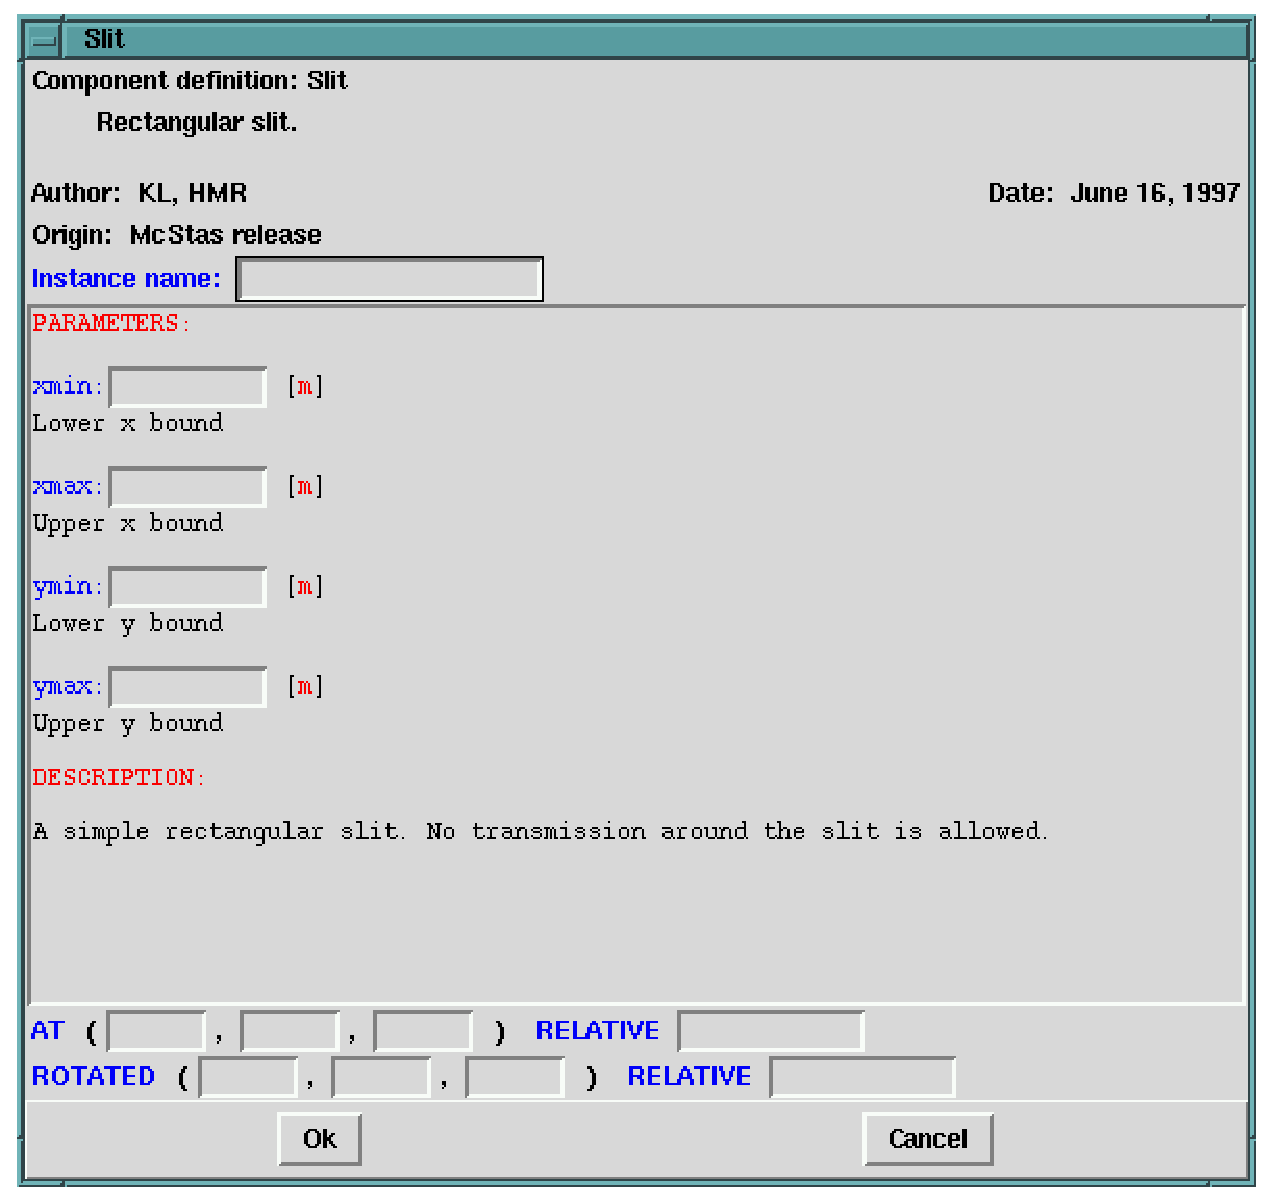
\includegraphics[width=0.55\textwidth]{figures/comp_dialog.eps}
    \caption{Component parameter entry dialog.}
    \label{f:comp_dialog}
  \end{center}
\end{figure}


To use the \verb+mcgui+ front-end, the programs Perl and Perl/Tk must be properly installed on the system.

Additionally, if the \MCS /PGPLOT back-end is used for data format, PGPLOT,
PgPerl, and PDL will be required. \index{Tools!Perl libraries} It may be
necessary to set the \verb+PGPLOT_DIR+ and \verb+PGPLOT_DEV+ environment
variable; consult the documentation for PGPLOT on the local system in case of
difficulty. \index{Environment variable!PGPLOT\_DIR} \index{Environment
variable!PGPLOT\_DEV}

\subsection{Running simulations with automatic compilation (mcrun)}
\label{s:mcrun}
\index{Tools!mcrun|textbf}
\index{Parameters!Instruments}
\index{Parameters!Scans}

The \verb+mcrun+ front-end (mcrun.pl on Windows) provides a convenient command-line
interface for running simulations with the same automatic compilation
features available in the \verb+mcgui+ front-end. It also provides a
facility for running a series of simulations while varying an input
parameter, thereby replacing the old \verb+gscan+ front-end.

The command
\begin{quote}
  \texttt{mcrun {\it sim} {\it args\/} \ldots}
\end{quote}
will compile the instrument definition \texttt{{\it sim}.instr} (if
necessary) into an executable simulation \texttt{{\it sim}.out}. It
will then run \texttt{{\it sim}.out}, passing the argument list {\it
  args}

The possible arguments are the same as those accepted by the simulations
themselves as described in section~\ref{s:run-sim}, with the following
extensions:
\begin{itemize}
\item The \verb+-c+ or \verb+--force-compile+ option may be used to force
  the recompilation of the instrument definition, regardless of file
  dates. This may be needed in case any component definitions are
  changed (in which case \verb+mcrun+ does not automatically recompile),
  or if a new version of McStas has been installed.
\item The \texttt{-p {\it file}} or \texttt{--param={\it file}} option
  may be used to specify a file containing assignment of values to the
  input parameters of the instrument definition. The file should consist
  of specifications of the form \texttt{{\it name\/}={\it value\/}}
  separated by spaces or line breaks. Multiple \verb+-p+ options may be
  given together with direct parameter specifications on the command
  line. If a parameter is assigned multiple times, later assignments
  override previous ones.
\item The \texttt{-N {\it count}} or \texttt{--numpoints={\it count}} option
  may be used to perform a series of \textit{count\/} simulations while
  varying one or more parameters within specified intervals. Such a
  series of simulations is called a \emph{scan}. To specify
  an interval for a parameter \textit{X}, it should be assigned two
  values separated with a comma. For example, the command
\begin{verbatim}
    mcrun sim.instr -N4 X=2,8 Y=1
\end{verbatim}
would run the simulation defined in \verb+sim.instr+ four times, with
\textit{X} having the values 2, 4, 6, and 8, respectively.

After running the simulation, the results will be written to the file
\verb+mcstas.dat+ by default. This file contains one line for each
simulation run giving the values of the scanned input variables along
with the intensity and estimated error in all detectors. Additionally, a
file \verb+mcstas.sci+ (when using Scialb format) is written that can be read by the \verb+mcplot+
front-end to plot the results on the screen or in a Postscript file, see
section~\ref{s:mcplot}. \index{Tools!mcplot}
\item When doing a scan, the \texttt{-f {\it file}} and
  \texttt{--file={\it file}} options make \verb+mcrun+ write the output
  to the files \texttt{{\it file\/}.dat} and \texttt{{\it file\/}.sim}
  instead of the default names.
\item When doing a scan, the \texttt{-d {\it dir}} and
  \texttt{--dir={\it dir}} options make \verb+mcrun+ put all output in a
  newly created directory \textit{dir}. Additionally, the directory will
  have subdirectories \verb+1+, \verb+2+, \verb+3+,\ldots containing all
  data files output from the different simulations. When the \verb+-d+
  option is not used, no data files are written from the individual
  simulations (in order to save disk space).
\item The \verb+mcrun --test+ command will test your \MCS\ installation, accuracy and plotter. \index{Installing}
\end{itemize}

The \verb+-h+ option will list valid options. The \verb+mcrun+ front-end requires a working installation of Perl to run.


\subsection{The \texttt{gscan} front-end}
\label{gscan}
\index{Tools!gscan (obsolete)}

The front-end \verb+gscan+ is obsolete from version~1.3 of McStas, and
is included only for backwards compatibility. The front-end~\verb+mcrun+
(section~\ref{s:mcrun}) includes all the functionality of the old
\verb+gscan+ front-end and should be used instead.


\subsection{Graphical display of simulations (mcdisplay)}
\label{s:mcdisplay}
\index{Tools!mcdisplay|textbf}

The front-end \verb+mcdisplay+ (mcdisplay.pl on Windows) is a graphical debugging tool.
It presents a schematic drawing of the instrument
definition, showing the position of the components and the paths of the
simulated neutrons through the instrument. It is thus very useful for
debugging a simulation, for example to spot components in the wrong
position or to find out where neutrons are getting lost.

To use the \verb+mcdisplay+ front-end with a simulation, run it as
follows:
\begin{quote}
  \verb+mcdisplay sim +{\it args \ldots}
\end{quote}
where \verb+sim+ is the name of either the instrument source \texttt{{\it sim}.instr} or the simulation program \texttt{{\it sim}.out} generated with
\MCS, and \textit{args \ldots} are the normal command line arguments for
the simulation, as explained above. The \verb+-h+ option will list valid options.

The drawing back-end program may be selected among PGPLOT, Matlab and Scilab using either the -p{\it PLOTTER} option or using the current \verb+MCSTAS_FORMAT+ environment variable. \index{Environment variable!MCSTAS\_FORMAT}
For instance, calling
\begin{quote}
  \verb+mcdisplay -pScilab ./vanadium_example.out ROT=90+
\end{quote}
or (\verb+csh+/\verb+tcsh+ syntax)
\begin{quote}
  \verb+setenv MCSTAS_FORMAT Scilab+\\
  \verb+mcdisplay ./vanadium_example.out ROT=90+
\end{quote}
will output graphics using Scilab.
The \verb+mcdisplay+ front-end can also be run from the \verb+mcgui+ front-end.
\index{Tools!mcgui}
Examples of plotter appearence for \verb+mcdisplay+ is shown in figures
 \ref{fig:mcdisp_PGPLOT}-\ref{fig:mcdisp_Matlab}.

\paragraph{\MCS /PGPLOT back-end}

This will view the instrument from above. A
multi-display that shows the instrument from three directions
simultaneously can be shown using the \verb+--multi+ option:
\begin{quote}
  \verb+mcdisplay --multi sim.out +{\it args \ldots}
\end{quote}

Click the left mouse button in the graphics window or hit the space key
to see the display of successive neutron trajectories. The `P' key saves
a postscript file containing the current display that can be sent to the
printer to obtain a hardcopy; the `C' key produces color postscript.
To stop the simulation
prematurely, type `Q' or use control-C as normal in the window in which
\verb+mcdisplay+ was started.

To see details in the instrument, it is possible to zoom in on a part of
the instrument using the middle mouse button (or the `Z' key on systems
with a one- or two-button mouse). The right mouse button (or the `X'
key) resets the zoom. Note that after zooming, the units on the
different axes may no longer be equal, and thus the angles as seen on
the display may not match the actual angles.

Another way to see details while maintaining an overview of the
instrument is to use the \verb+--zoom=+\textit{factor} option. This
magnifies the display of each component along the selected axis only,
{\em e.g.} a Soller collimator is magnified perpendicular to the neutron beam
but not along it. This option may produce rather strange visual effects
as the neutron passes between components with different coordinate
magnifications, but it is occasionally useful.

When debugging, it is often the case that one is interested only in
neutrons that reach a particular component in the instrument. For
example, if there is a problem with the sample one may prefer not to see
the neutrons that are absorbed in the monochromator shielding. For these
cases, the \verb+--inspect=+\textit{comp\/} option is useful. With this
option, only neutrons that reach the component named \textit{comp\/} are
shown in the graphics display.

The \verb+mcdisplay+ front-end will then require the Perl, the PGPLOT, and the
PGPerl packages to be installed. It may be necessary to set the
\verb+PGPLOT_DIR+ and \verb+PGPLOT_DEV+ environment variable; consult the
documentation for PGPLOT on the local system in case of difficulty.
\index{Environment variable!PGPLOT\_DIR} \index{Environment
variable!PGPLOT\_DEV} \index{Tools!Perl libraries}

\paragraph{Matlab and Scilab back-ends}

A 3D view of the instrument, and various operations (zoom, export, print, trace neutrons, \ldots) is available from dedicated Graphical User Interfaces.
The \verb+--inspect+ option may be used (see previous paragraph), as well as the \verb+--first+ and \verb+--last+ options to specify a region of interest. {\bf Note:} The Scilab plotter for \emph{Windows} does not allow to rotate interactively the 3D view, and you are to use the \emph{alpha} and \emph{theta} choices in the pop-up Dialog.

The \verb+mcdisplay+ front-end will then
require the Perl+PGPLOT, and either Scilab or Matlab to be installed. \index{Tools!Matlab} \index{Tools!Scilab}

See section~\ref{s:comp-mcdisplay} for how to make new components work
with the \verb+mcdisplay+ front-end.

\subsection{Plotting the results of a simulation (mcplot)}
\label{s:mcplot}
\index{Tools!mcplot|textbf}

The front-end \verb+mcplot+ (mcplot.pl on Windows) is a program that produces
plots of all the detectors in a simulation, and it is thus useful to get
a quick overview of the simulation results.

In the simplest case, the front-end is run simply by typing
\begin{verbatim}
    mcplot
\end{verbatim}
This will plot any simulation data stored in the current directory,
which is where simulations put their results by default. If the
\verb+--dir+ or \verb+--file+ options have been used (see
section~\ref{s:run-sim}), the name of the file or directory should be
passed to mcplot, {\em e.g.} ``\texttt{mcplot {\it dir}}'' or ``\texttt{mcplot
  {\it file}}''.
It is also possible to plot one single text (not binary) data file from a given monitor, passing its name to mcplot.

The drawing back-end program may be selected among PGPLOT, Matlab and Scilab using either the -p{\it PLOTTER} option (e.g. \verb+mcplot -pScilab file+) or using the current \verb+MCSTAS_FORMAT+ environment variable. \index{Environment variable!MCSTAS\_FORMAT} Moreover, the drawing back-end program will also be set depending on the {\it file} extension (see table~\ref{t:formatoptions}).

It should be emphasized that \verb+mcplot+ may \emph{only} display simulation results with the format that was chosen during the computation. Indeed, if you request data in a given format from a simulation, you will only be able to display results using that same drawing back-end. Anyway, the \verb+mcconvert+ utility may convert a \MCS\ data file between Matlab and Scilab formats (see section \ref{s:mcconvert}).

The \verb+mcplot+ front-end can also be run from the \verb+mcgui+ front-end.
\index{Tools!mcgui}

The initial display shows plots for each detector in the simulation.
Examples of plotter appearence for \verb+mcplot+ is shown in figures
 \ref{fig:mcdisp_PGPLOT}-\ref{fig:mcplot_figs}.

\paragraph{\MCS /PGPLOT back-end}

Clicking the left mouse button on a plot produces a full-window version
of that plot. The `P' key saves a postscript file containing the current
plot that can be sent to the printer to obtain a hardcopy; the `C' key
produces color postscript.
The `Q' key quits the program (or CTRL-C in the controlling
terminal may be used as normal).

To use the \verb+mcplot+ front-end with PGPLOT, the programs Perl, PGPLOT,
PgPerl, and PDL must all be properly installed on the system.  It may be
necessary to set the \verb+PGPLOT_DIR+ and \verb+PGPLOT_DEV+ environment
variable; consult the documentation for PGPLOT on the local system in case of
difficulty. \index{Environment variable!PGPLOT\_DIR} \index{Environment
variable!PGPLOT\_DEV} \index{Tools!Perl libraries}

\paragraph{Matlab and Scilab back-ends}

A dedicated \MCS /Mcplot Dialog or menu attached to the plotting window is available, and provides many operations (duplication, export, colormaps, \ldots).
The corresponding 'mcplot' Matlab and Scilab functions may be called from these language prompt with the same method as in section~\ref{s:run-sim}, e.g:
\begin{verbatim}
    matlab> s=mcplot;
    matlab> help mcplot
    scilab> s=mcplot();
    matlab or scilab> s=mcplot('mcstas.m');
    matlab or scilab> mcplot(s);
\end{verbatim} \index{Tools!Matlab} \index{Tools!Scilab}
A full parameter scan simulation result, or simply one of its scan steps may be displayed using the 'Scan step' menu item.
When the \verb|+nw| option is specified, a separate Matlab or Scilab window will appear (instead of being launched in the current terminal). This will then enable Java support under Matlab and Tk support under Scilab, resulting in additional menus and tools.

To use the \verb+mcplot+ front-end, the programs Perl, and either Scilab or Matlab are required. \index{Tools!Matlab} \index{Tools!Scilab}


\subsection{Plotting resolution functions (mcresplot)}
\label{s:mcresplot}
\index{Tools!mcresplot|textbf}

\begin{figure}[htb!]
  \begin{center}
    \includegraphics[angle=-90,width=0.55\textwidth]{figures/mcresplot_PGPLOT.ps}
  \end{center}
\caption{Output from \texttt{mcresplot} with PGPLOT backend.
  Use P, C and G keys to write hadrcopy files.}
\label{fig:mcresplot_PGPLOT}
\end{figure}

The \verb+mcresplot+ front-end is used to plot the resolution function, particularly for triple-axis
%or inverse geometry time-of-flight
spectrometers, as
calculated by the Res\_sample component. It requires to have a Res\_monitor component further in the instrument description (at the detector position).
%(see section~\ref{s:res_sample}).
This front-end
has been included in the release since it may be useful
despite its somewhat rough user interface.

The \verb+mcresplot+ front-end is launched with the command
\begin{quote}
  \texttt{mcresplot {\it file\/}}
\end{quote}
Here, {\it file\/} is the name of a file output from a simulation using
the Res\_monitor component.
% (section~\ref{s:res_monitor}).

This front-end currently only works with the PGPLOT plotter, but ports for Matlab and Scilab may be written in the future.

The front-end will open a window displaying projections of the 4-dimensional
resolution function $R(\boldsymbol{Q}, \omega)$. The covariance matrix of the
resolution function, the resolution along each projection axis and the resulting
resolution matrix are also shown, as well as the instrument name and parameters
used for the simulation. This is mainly useful for triple-axis spectrometers.

To use the \verb+mcresplot+ front-end, the programs Perl, PGPLOT, PgPerl,
and PDL must all be properly installed on the system.
\index{Tools!Perl libraries}

\subsection{Creating and viewing the library and component/instrument help (mcdoc)}
\label{s:mcdoc-run}
\index{Tools!mcdoc|textbf}

\MCS\ provides an easy way to generate automatically an HTML help page about a given component or instrument, or the whole \MCS\ library. \index{Library!Components}
\begin{quote}
  \verb|mcdoc|\\
  \verb|mcdoc| {\it comp|instr}\\
  \verb|mcdoc -l|
\end{quote}
The first example generates an {\it index.html} catalog file using the available components and instruments (both locally, and in the \MCS\ library. When called with the \verb+--show+ or \verb+-s+ option, the library catalog of components is opened using the \verb+BROWSER+ environment variable \index{Environment variable!BROWSER} (e.g. netscape, konqueror, nautilus, MSIE, mozilla, \ldots).

Alternatively, if a component or instrument {\it comp} is specified, it will be searched within the library, and an HTML help will be created for all available components matching {\it comp}. When using the \verb+-s+, the help will be opened. If the \verb+BROWSER+ is not defined, the help is displayed as text in the current terminal. This latter output may be forced with the \verb+-t+ or \verb+--text+ option.

The last example will list the name and action of all \MCS\ tools (same as \verb+--tools+ option).

Additionally, the \verb+--web+, \verb+--manual+ and \verb+--comp+ options will open the \MCS\ web site page, the User Manual (this document) and the Component Manual, all requiring \verb+BROWSER+ to be defined. Finally, the \verb+--help+ option will display the command help, as usual.

See section~\ref{s:mcdoc} for more details about the McDoc usage and header format.
To use the \verb+mcdoc+ front-end, the program Perl should be available.

\subsection{Translating \MCS\ components for Vitess (mcstas2vitess)}
\label{s:mcstas2vitess}
\index{Tools!mcstas2vitess|textbf}
\index{Library!vitess-lib}

Any \MCS\ component may be translated for usage with Vitess (starting from version 2.3). The syntax is simply \index{Library!Components}
\begin{quote}
  \texttt{mcstas2vitess {\it file.comp\/}}
\end{quote}
This will create a Vitess module of the given component.
To use the \verb+mcstas2vitess+ front-end, the program Perl should be available.

\subsection{Translating \MCS\ results files between Matlab and Scilab formats}
\label{s:mcconvert}
\index{Tools!mcconvert|textbf}
\index{Tools!Matlab} \index{Tools!Scilab}

If you have been running a \MCS\ simulation with Scilab output, but finally plan to look at the results with Matlab, or the contrary, you may use
\begin{quote}
  \texttt{mcconvert {\it file.{m|sci}\/}}
\end{quote}
to simply translate one file format the other. This works only for the text files of course. The binary files need not be translated.

\section{Analyzing and visualizing the simulation results}
\label{s:analyze}
\index{Data format}

To analyze simulation results, one uses the same tools as for analyzing
experimental data, \textit{i.e}. programs such as IDL, Matlab and Scilab.
The output files from simulations are usually simple text files containing headers and data blocks. If data blocks are empty they may be accessed refering to an external file indicated in the header. This file may also be a binary file (except with the original \MCS /PGPLOT format), which does not contain any header (except if simulation is launched with \verb|+a| option), but are in turn smaller in size and faster to import.

In order for the user to choose the data format, we recommand to set it {\it via} the MCSTAS\_FORMAT environment variable, which will also make the front-end programs able to import and plot data and instrument consistently. The available format list is shown in table~\ref{t:formatoptions}. \index{Environment variable!MCSTAS\_FORMAT}


Note that the neutron event counts in detectors is typically not very
meaningful except as a way to measure the performance of the
simulation. Use the simulated intensity instead whenever analysing
simulation data.

\paragraph{\MCS\ and PGPLOT format}

The \MCS\ original format, which is equivalent to the PGPLOT format, is simply columns of ASCII text that most programs should
be able to read.

One-dimensional histogram detectors (time-of-flight, energy-sensitive)
write one line for each histogram bin. Each line contains a number
identifying the bin (\textit{i.e}.\ the time-of-flight) followed by
three numbers: the simulated intensity, an estimate of the statistical
error as explained in section~\ref{s:staterror}, and the number of
neutron events for this bin.

Two-dimensional histogram detectors (position sensitive detectors)
output $M$ lines of $N$ numbers representing neutron intensities, where
$M$ and $N$ are the number of bins in the two dimensions. The
two-dimentional detectors also store the error estimates and event counts as additional matrices.

Single-point detectors output the neutron intensity, the estimated
error, and the neutron event count as numbers on the
terminal. (The results from a series of simulations may be combined in a
data file using the \verb+mcrun+ front-end as explained in
section~\ref{s:mcrun}).

Both one- and two-dimentional detector output by default start with a
header of comment lines, all beginning with the `\verb+#+' character.
This header gives such information as the name of the instrument used in
the simulation, the values of any instrument parameters, the name of the
detector component for this data file, \textit{etc}. The headers may be
disabled using the \verb+--data-only+ option in case the file must be
read by a program that cannot handle the headers.

In addition to the files written for each one- and two-dimensional
detector component, another file (by default named \verb+mcstas.sim+) is
also created. This file is in a special \MCS\ ASCII format. It contains
all available information about the instrument definition used for the
simulation, the parameters and options used to run the simulation, and
the detector components present in the instrument. It is read by the
\verb+mcplot+ front-end (see section~\ref{s:mcplot}). This file stores
the results from single detectors, but by default contains only pointers
(in the form of file names) to data for one- and two-dimensional
detectors. By storing data in separate files, reading the data with
programs that do not know the special \MCS\ file format is
simplified. The \verb+--file+ option may be used to store all data
inside the \verb+mcstas.sim+ file instead of in separate files.

\paragraph{Matlab, Scilab and IDL formats}
\index{Tools!Matlab} \index{Tools!Scilab} \index{Tools!IDL} \index{Data format}

These formats write automatically scripts containing the data as a structure, as well as in-line import and plot functions for the selected language. Usage examples are given in section~\ref{s:run-sim}.
Thus, it is not necessary to write a load routine for each format, as the script is itself a program that knows how to handle the data. Alternatively, using \verb+mcplot+ with Matlab and Scilab plotters provide additional functionalities from menus and dialogs (see section~\ref{s:mcplot}).

When imported through the data generated script (see section~\ref{s:run-sim}), or using \verb+mcplot+ (see section~\ref{s:mcplot}), a single variable may be created into the Matlab, Scilab or IDL base workspace. This variable is a \emph{structure} constituting a data tree containing many fields, some of them being themselves structures. Field names are the initial names from the instrument (components, files, \ldots), transformed into valid variable names, e.g containing only letters, digits and the '\_' character, except for the first character which may only be a letter, or the 'm' letter\footnote{For instance in most case, the simulation location is './mcstas.m' which turns into field 'm\_mcstas'.}.
In this tree, you will find the monitor names, which fields contain the monitored data. The usual structure is
\begin{quote}
  \texttt{s.{\it instrument}.{\it simulation}.{\it comp\_name}.{\it file\_name}}
\end{quote}

For instance, reading the data from a 'test' instrument using Matlab format will look like
\begin{verbatim}
matlab> s=mcstas; % or mcplot mcstas.m from the terminal
matlab> s
s =
     Format: 'Matlab with text headers'
        URL: 'http://neutron.risoe.dk'
     Editor: 'farhi on pcfarhi'
    Creator: 'test (test.instr) McStas 1.7 - May. 14, 2003 simulation'
       Date: 1.0529e+09
       File: './mcstas'
       test: [1x1 struct]
    EndDate: 1.0529e+09
      class: 'root'
matlab> s.test.m_mcstas.monitor1.monitor1_y_kz
ans =
          ...
          Date:       1.0529e+09
          File:       'monitor1.y_kz'
          type:       'array_2d(20, 10)'
          ...
          ratio:      '1e+06/1e+06'
          signal:     'Min=0; Max=5.54051e-10; Mean= 6.73026e-13;'
          statistics: 'X0=0.438302; dX=0.0201232; Y0=51019.6; dY=20557.1;'
          ...
matlab> eval(s.test.m_mcstas.monitor1.monitor1_y_kz);
matlab> dX
ans =
          0.0201232
\end{verbatim}
The latter example accesses the data from the 'monitor1.y\_kz' file written by the 'monitor1' component in the 'test' instrument during the './mcstas' simulation. You may evaluate directly the 'signal' and 'statistics' fields of the structure to obtain useful informations.

\paragraph{HTML, XML/NeXus and NeXus formats}

Both HTML and XML/NeXus formats are available. The former may be viewed using any web browser (Netscape, Internet Explorer, Nautilus), while the latter may be browsed for instance using Internet Explorer (Windows and Mac OS) or GXMLViewer and KXMLEditor (under Linux).

A future version of \MCS\ will support output in the NeXus
format~\cite{nexus_webpage}.

% Emacs settings: -*-mode: latex; TeX-master: "manual.tex"; -*-

\chapter{The \MCS kernel and meta-language}
\label{s:kernel}
\index{Kernel|textbf}

Instrument definitions are written in a special \MCS meta-language which
is translated automatically by the \MCS compiler into a C program
which is in turn compiled to an executable that
performs the simulation. The meta-language is custom-designed for neutron
scattering and serves two main purposes: (i) to specify the interaction of a
single neutron ray with a single optical component, and (ii) to build a
simulation by constructing a complete instrument from individual
components.

For maximum flexibility and efficiency, the meta-language is based on C.
Instrument geometry, propagation of neutrons between the different
components, parameters, data input/output etc.\ is handled in the
meta-language and by the \MCS compiler. Complex calculations are written in
C embedded in the meta-language description of the
components. However, it is
possible to set up an instrument from existing components and
run a simulation without writing a single line of C code, working
entirely in the meta-language.

Apart from the meta-language, \MCS also includes a number of C library
functions and definitions that are useful for neutron ray-tracing
simulations. 
% FIXME File not found
% The definitions available for component developers are listed in appendix~\ref{c:kernelcalls}. 
The list includes functions for
\begin{itemize}
\item Computing the intersection between a flight-path and various
  objects (such as planes, cylinders, boxes and spheres)
\item Functions for generating random numbers
with various distributions
\item Functions for reading or writing informations from/to data
  files
\item Convenient conversion factors between relevant units, etc.
\index{Library!Run-time}
\index{Library!Components!share}
\end{itemize}

The \MCS meta-language was designed to be readable, with a verbose
syntax and explicit mentioning of otherwise implicit information. The
recommended way to get started with the meta-language is to start by
looking at the examples supplied with \MCS, modifying them as necessary
for the application at hand.

\section{Notational conventions}

Simulations generated by \MCS use a semi-classical description of the
neutron rays to compute the neutron trajectory through the instrument and its
interaction with the different components. The effect of gravity is
taken  into account either in particular components (e.g. \verb+Guide_gravity+), or more generaly
when setting an execution flag (\verb+-g+) to perform gravitation
computation. This latter setting is only an approximation and may produce
wrong results with some components.\index{Gravitation}

An instrument consists of a list of components through which the neutron
ray passes one after the other. The order of components is thus significant
since \MCS does not automatically check which component is the next to
interact with the neutron ray at a given point in the simulation. Note
that in case of a negative propagation time from one component to the
next, the neutron ray is by default \emph{absorbed} as this is often
an indication of unphysical conditions.

The instrument is given a global, absolute coordinate system. In
addition, every component in the instrument has its own local coordinate
system that can be given any desired position and orientation (though
the position and orientation must remain fixed for the duration of a
single simulation). \index{Coordinate system}
By convention, the $z$ axis points in the direction of the beam, the $x$ axis
is perpendicular to the beam in the horizontal plane pointing left as seen
from the source, and the $y$ axis points upwards (see figure~\ref{f:axis}).
Nothing in the \MCS metalanguage enforces this convention, but if every component used
different conventions the user would be faced with a severe headache! It is
therefore necessary that this convention is followed by users implementing
new components.
\begin{figure}
  \begin{center}
    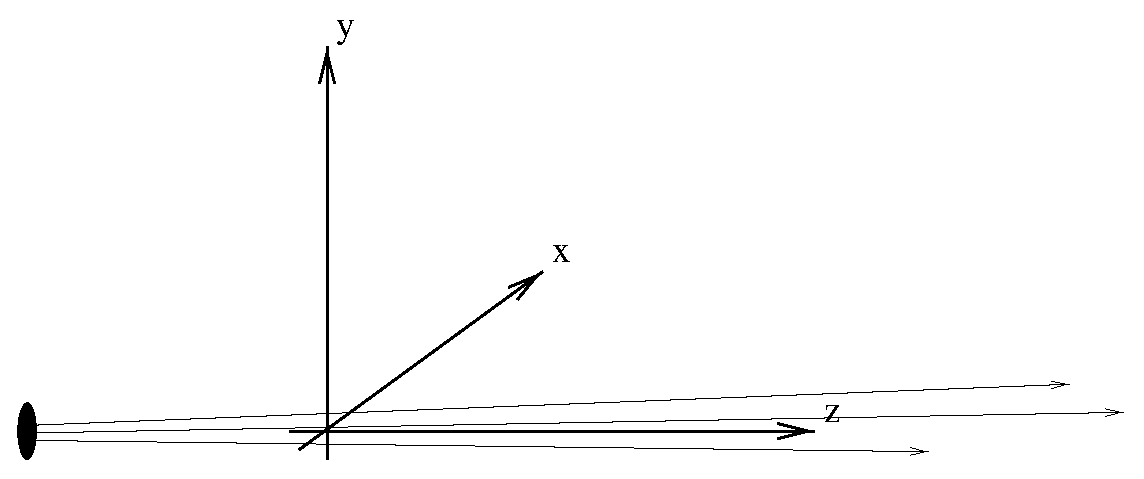
\includegraphics[width=0.8\textwidth]{figures/axis-conventions.eps}
  \end{center}
\caption{conventions for the orientations of the axis in simulations.}
\label{f:axis}
\end{figure}

\index{Neutron state and units}
In the instrument definitions, units of length (\textit{e.g}.\ component
positions) are given in meters and units of angles (\textit{e.g}.\
rotations) are given in degrees.  The state of the neutron is given by
its position $(x,y,z)$ in meters, its velocity $(v_x, v_y, v_z)$ in
meters per second, the time $t$ in seconds, and the three spin parameters
$\left( s_x, s_y, s_z \right)$, and finally the neutron weight $p$ described in \ref{s:MCtechniques}.

\section{Syntaxical conventions}
\label{s:syntax}

Comments follow the normal C syntax ``\verb+/* ... */+''. C++ style
comments ``\verb+// ...+'' may also be used.
\index{Comments}

%For backward-compatibility
%with early versions, comments may also be written as a percentage sign
%followed by a space (``\verb*+% ...+''), but this is not recommended and
%will be removed in a future version.

Keywords are not case-sensitive, for example ``\verb+DEFINE+'',
``\verb+define+'', and ``\verb+dEfInE+'' are all equivalent. However, by
convention we always write keywords in uppercase to distinguish them
from identifiers and C language keywords. In contrast, \MCS
identifiers (names), like C identifiers and keywords, \emph{are} case
sensitive, another good reason to use a consistent case convention for
keywords. All \MCS keywords are reserved, and thus should not be used
as C variable names. The list of these reserved keywords is shown in table~\ref{t:keywords}. \index{Keyword}

\begin{table}
  \begin{center}
    {\let\my=\\
    \begin{tabular}{|l|c|p{0.7\textwidth}|}
      \hline
      \texttt{Keyword} & Scope & Meaning \\
      \hline
      \texttt{ABSOLUTE} & I & Indicates that the AT and ROTATED keywords are in the absolute coordinate system. \\
      \texttt{AT} & I & Indicates the position of a component in an instrument definition. \\
      \texttt{COPY}& I,C & copy/duplicate an instance or a component definition. \\
      \texttt{DECLARE} & I,C & Declares C internal variables. \\
      \texttt{DEFINE} & I,C & Starts an INSTRUMENT or COMPONENT definition. \\
      \texttt{DEFINITION} & C & Defines component parameters that are constants (\#define). \\
      \texttt{END} & I,C & Ends the instrument or component definition. \\
      \texttt{SPLIT} & I & Enhance incoming statistics by event repetition. \\
      \texttt{EXTEND} & I & Extends a component TRACE section (plug-in). \\
      \texttt{FINALLY} & I,C & Embeds C code to execute when simulation ends. \\
      \texttt{GROUP} & I & Defines an exclusive group of components. \\
      \texttt{\%include} & I,C & Imports an instrument part, a component or a piece of C code (when within embedded C). \\
      \texttt{JUMP} & I & Iterative (loops) and conditional jumps. \\
      \texttt{INITIALIZE} & I,C & Embeds C code to be executed when starting. \\
      \texttt{ITERATE} & I & Defines iteration counter for JUMP. \\
      \texttt{MCDISPLAY} & C & Embeds C code to display component geometry. \\
      \texttt{NEXUS} & I & Defines NeXus output type (4,5,XML,compression). \\
      \texttt{OUTPUT} & C & Defines internal variables to be public and protected symbols (usually all global variables and functions of DECLARE).\\
      \texttt{PARAMETERS} & C & Defines a class of component parameter (DEFINITION, SETTING). \\
      \texttt{POLARISATION} & C & Defines neutron polarisation coordinates. \\
      \texttt{PREVIOUS} & C & Refers to a previous component position/orientation.\\
      \texttt{RELATIVE} & I & Indicates that the AT and ROTATED keywords are relative to an other component. \\
      \texttt{REMOVABLE} & I & Indicates that this component will be removed when the instrument is inserted into an other one using the \texttt{\%include} keyword. \\
      \texttt{ROTATED} & I & Indicates the orientation of a component in an instrument definition. \\
      \texttt{SAVE} & I,C & Embedded C code to execute when saving data. \\
      \texttt{SETTING} & C & Defines component parameters that are
      variables. \\
      \texttt{SHARE} & C & Declares global functions and variables to be shared. \\
      \texttt{TRACE} & I,C & Defines the instrument as a the component sequence. \\
      \texttt{WHEN}  & I & Condition for component activation and JUMP.\\
      \hline
    \end{tabular}
    \caption{Reserved \MCS keywords.
    Scope is 'I' for instrument and 'C' for component definitions.}
    \label{t:keywords}
    }
  \end{center}
\end{table}

It is possible, and usual, to split the input instrument definition
across several different files. For example, if a component is not
explicitly defined in the instrument,
\MCS will search for a file containing the component definition in the
standard component library (as well as in the current directory and any
user-specified search directories, see section~\ref{s:files}). It is
also possible to explicitly include another file using a line of the
form \index{Keyword!\%include}
\begin{lstlisting}
    %include "file"
\end{lstlisting}
Beware of possible confusion with the C language ``\verb+#include+''
statement, especially when it is used in C code embedded within the
\MCS meta-language. Files referenced with ``\verb+%include+'' are read
when the instrument is translated into C by the \MCS compiler, and must
contain valid \MCS meta-language input (and possibly C code). Files referenced with
``\verb+#include+'' are read when the C compiler generates an
executable from the generated C code, and must contain valid C.

Embedded C code is used in several instances in the \MCS
meta-language. Such code is copied by the \MCS compiler into the
generated simulation C program. Embedded C code is written by putting it
between the special symbols \verb|%{| and \verb|%}|, as follows:
\begin{quote}
  \verb|%{| \\
  \hbox to 3em{}\ldots Embedded C code \ldots \\
  \verb|%}|
\end{quote} \index{Embedded C code}
The ``\verb|%{|'' and ``\verb|%}|'' must appear on a line by themselves (do not add comments after).
Additionally, if a ``\verb+%include+'' statement is found \emph{within} an embedded C code block, the specified file will be included from the 'share' directory of the standard component library \index{Library!Components!share} (or from the
current directory and any user-specified search directories) as a C library, just like the usual ``\verb+#include+'' \emph{but only once}. For instance, if many components require to read data from a file, they may all ask for ``\verb+%include "read_table-lib"+'' \index{Library!read\_table-lib (Read\_Table)} without duplicating the code of this library. If the file has no extension, both \verb+.h+ and \verb+.c+ files will be searched and included, otherwise, only the specified file will be imported. The \MCS 'run-time' shared
library is included by default (equivalent to ``\verb+%include "mcstas-r"+'' in the \texttt{DECLARE} section). \index{Library!Run-time}
For an
example of \texttt{\%include}, see the monitors/Monitor\_nD component. See also section \ref{s:instrdefs-extend} for insertion of full instruments in instruments (instrument catenation).

If the instrument description compilation fails, check that the
keywords syntax is correct, that no semi-colon \verb+;+ sign is
missing (e.g. in C blocks and after an ABSORB macro), and there are no name conflicts between instrument and component instances variables.\index{Can not compile}


\section{Writing instrument definitions}
\label{s:instrdefs}
\index{Instruments}

The purpose of the instrument definition is to specify a sequence of
components, along with their position and parameters, which together
make up an instrument. Each component is given its own local coordinate
system, the position and orientation of which may be specified by its
translation and rotation relative to another component. 
% FIXME An example is given in section~\ref{s:Samples_vanadium.instr} and some additional examples of instrument definitions can be found on the McStas web-page~\cite{mcstas_webpage} and in the \texttt{example} directory.

As a summary, the usual grammar for instrument descriptions is
\begin{lstlisting}
DEFINE INSTRUMENT name(parameters)
DECLARE C_code
INITIALIZE C_code {NEXUS}
TRACE components
{FINALLY C_code}
END
\end{lstlisting}


\subsection{The instrument definition head}

\begin{quote}
  \texttt{DEFINE} \texttt{INSTRUMENT} \textit{name} $(a_1, a_2, \ldots)$
\end{quote} \index{Keyword!DEFINE!INSTRUMENT}
This marks the beginning of the definition. It also gives the name of
the instrument and the list of instrument parameters. Instrument
parameters describe the configuration of the instrument, and usually
correspond to setting parameters of the components, see section \ref{s:compdefs}. A motor position is
a typical example of an instrument parameter. The input parameters of
the instrument constitute the input that the user (or possibly a
front-end program) must supply when the
generated simulation is started.

\index{Parameters!Instruments}
By default, the parameters will be floating point numbers, and will have
the C type \verb+double+ (double precision floating point). The type of
each parameter may optionally be declared to be \verb+int+ for the C
integer type or \verb+char *+ for the C string type. The name
\verb+string+ may be used as a synonym for \verb+char *+, and floating
point parameters may be explicitly declared using the name
\verb+double+. The following example illustrates all possibilities:
\begin{quote}
  \texttt{DEFINE INSTRUMENT test(d1, double d2, int i, char *s1, string s2)}
\end{quote}
Here \verb+d1+ and \verb+d2+ will be floating point parameters of C type
\verb+double+, \verb+i+ will be an integer parameter of C type
\verb+int+, and \verb+s1+ and \verb+s2+ will be string parameters of C
type \verb+char *+.
\index{Parameters!Optional, default value}
The parameters of an instrument may be given default values. Parameters with default values are called \emph{optional
  parameters}, and need not be given an explicit value when the
instrument simulation is executed. When executed without any parameter value in the command line (see section~\ref{s:run-sim}), the instrument asks for all parameter values, but pressing the \verb+Return+ key selects the default value (if any). When used with at least one parameter value in the command line, all non specified parameters will have their value set to the default one (if any). A parameter is given a
default value using the syntax ``\textit{param}\texttt{= }\textit{value}''.
For example
\begin{quote}
  \texttt{DEFINE INSTRUMENT test(d1= 1, string s2="hello")}
\end{quote}
Here \verb+d1+ and \verb+d2+ are optional parameters and if no
value are given explicitly, ``1'' and ``hello'' will be used.

Optional parameters can greatly increase the convenience for users of
instruments for which some parameters are seldom changed or of unclear signification to the user. Also, if all instrument parameters have default values, then the simple command \verb+mcdisplay+ \verb+test.instr+ will show the instrument view without requesting any other input, which is usually a good starting point to study the instrument design.

\subsection{The \texttt{DECLARE} section}
\index{Keyword!DECLARE}
\label{s:declare}

\begin{quote}
  \texttt{DECLARE} \\
  \verb|%{| \\
  \hbox to 3em{}\ldots C declarations of global variables etc. \ldots \\
  \verb|%}|
\end{quote} \index{Embedded C code}
This gives C declarations that may be referred to in the rest of the
instrument definition. A typical use is to declare global variables or
small functions that are used elsewhere in the instrument. The \verb+%include ''file''+ keyword may be used to import a specific
component definition or a part of an instrument. Variables defined here are global, and may conflict with internal \MCS variables, specially symbols like \verb+x,y,z,sx,sy,sz,vx,vy,vz,t+ and generally all names starting with \verb+mc+ should be avoided. If you can not compile the instrument, this may be the reason. \index{Can not compile}The \texttt{DECLARE} section is optional.

\subsection{The \texttt{INITIALIZE} section}
\index{Keyword!INITIALIZE}
\label{s:initialize}

\begin{quote}
  \texttt{INITIALIZE} \\
  \verb|%{| \\
  \hbox to 3em{}\ldots C initializations. \ldots \\
  \verb|%}|
\end{quote} \index{Embedded C code}
This gives code that is executed when the simulation starts. This section is
optional. Instrument setting parameters may be modified in this section (e.g. doing tests or automatic settings).

\subsection{The \texttt{NEXUS} extension}
\index{Keyword!NEXUS} \index{Tools!NeXus} \index{Tools!HDF} \index{Data formats}
\label{s:nexus}

The NeXus format~\cite{nexus_webpage} requires to link the simulation to additional libraries (HDF and NeXus) which must have been pre-installed. Preferably, \MCS should have been installed with the \verb+./configure --with-nexus+ on Unix/Linux systems. To activate the NeXus output, the compilation of the instrument must be done with flag \verb+-DUSE_NEXUS -lNeXus+. The resulting executable is no longer portable.

The default NeXus format is NeXus 5 with compression. However, that format may be changed with the optional keyword \verb+NEXUS+ to follow the INITIALIZE section, namely:

\begin{quote}
  \texttt{INITIALIZE} \\
  \verb|%{| \\
  \hbox to 3em{}\ldots C initializations. \ldots \\
  \verb|%}|
  \verb+NEXUS {"4"|"5"|"XML"|"compress"|"zip"}+
\end{quote}

It is possible to set the type of NeXus file with a string argument, containing words "4", "5" or "XML". Optionally, if the string also contains the \verb+compress+ or \verb+zip+ word, the NeXus file will use compression for Data Sets. We recommend the syntax \verb+NEXUS "5 compress"+ which is the default.

You may choose the name of the output file with the \verb+-f filename+ option from the instrument executable or \verb+mcrun+ (see Sections \ref{s:run-sim}, \ref{s:mcrun} and Table \ref{f:simoptions2}).

Then, the output format is chosen as usual with the \verb+--format=NeXus+ option when launching the simulation. All output files are stored in the output {\it filename}, as well as the instrument description itself. Other formats are still available. When run on a distributed system (e.g. MPI), detectors are gathered, but list of events (see e.g. component Virtual\_output) are stored as one data set per node.

\subsection{The \texttt{TRACE} section}
\index{Keyword!TRACE}
\label{s:trace}


As a summary, the usual grammar for component instances within the instrument TRACE section is
\begin{lstlisting}
COMPONENT name = comp(parameters)
  AT (...) [RELATIVE [reference|PREVIOUS] | ABSOLUTE]
 {ROTATED  {RELATIVE [reference|PREVIOUS] | ABSOLUTE} }
\end{lstlisting}

The \texttt{TRACE} keyword starts a section giving the list of
components that constitute the instrument.
Components are declared like this:
\begin{quote}
  \texttt{COMPONENT} $\textit{name} =
    \textit{comp}(p_1 = e_1, p_2 = e_2, \ldots)$
\end{quote}
\index{Components}
\index{Keyword!COMPONENT} \index{Parameters!Setting}
\index{Parameters!Definition}
This declares a component named \textit{name} that is an instance of the
component definition named \textit{comp}. The parameter list gives the
setting and definition parameters for the component. The expressions $e_1,
e_2, \ldots$ define the values of the parameters. For setting parameters
arbitrary ANSI-C expressions may be used, while for definition parameters
only \emph{constant} numbers, strings, names of instrument parameters, or names
of C identifiers are allowed (see section~\ref{s:comp-header} for details of
the difference between definition and setting parameters). To assign the
value of a general expression to a definition parameter, it is necessary to
declare a variable in the \texttt{DECLARE} section, assign the value to the
variable in the \texttt{INITIALIZE} section, and use the variable as the
value for the parameter.

The \MCS program takes care to rename parameters appropriately in the
output so that no conflicts occur between different component
definitions or between component and instrument definitions. It is thus
possible (and usual) to use a component definition multiple times
in an instrument description.

Beware about variable type conversion when setting numerical parameter values, as in \verb+p1=12/1000+. In this example, the parameter \verb+p1+ will be set to 0 as the division of the two integers is indeed 0. To avoid that, use explicitely floating type numbers as in \verb+p1=12.0/1000+.\index{Bugs}

The \MCS compiler will automatically search for a file containing a
definition of the component if it has not been declared previously. The
definition is searched for in a file called ``{\it name\/}{\tt .comp}''. See
section~\ref{s:files} for details on which directories are searched. This
facility is often used to refer to existing component definitions in
standard component libraries. It is also possible to write component
definitions in the main file before the instrument definitions, or to
explicitly read definitions from other files using \verb+%include+
(not within embedded C blocks).

The physical position of a component is specified using an \texttt{AT} modifier
following the component declaration:
\index{Keyword!AT} \index{Keyword!RELATIVE} \index{Keyword!ABSOLUTE}
\begin{quote}
  \texttt{AT} $(x,y,z)$ \texttt{RELATIVE} \textit{name}
\end{quote}
This places the component at position $(x,y,z)$ in the coordinate system
of the previously declared component \textit{name}. Placement may also
be absolute (not relative to any component) by writing
\begin{quote}
  \texttt{AT} $(x,y,z)$ \texttt{ABSOLUTE}
\end{quote}
Any C expression may be used for $x$, $y$, and $z$. The \texttt{AT}
modifier is required.
Rotation is achieved similarly by writing \index{Keyword!ROTATED}
\begin{quote}
  \texttt{ROTATED} $(\phi_x,\phi_y,\phi_z)$ \texttt{RELATIVE} \textit{name}
\end{quote}
This will result in a coordinate system that is rotated first the angle
$\phi_x$ (in degrees) around the $x$ axis, then $\phi_y$ around the $y$ axis, and finally
$\phi_z$ around the $z$ axis. Rotation may also be specified using
\texttt{ABSOLUTE} rather than \texttt{RELATIVE}. If no rotation is
specified, the default is $(0,0,0)$ using the same relative or absolute
specification used in the \texttt{AT} modifier. We \emph{highly} recommand to apply all rotations of an instrument description on Arm class components only, acting as goniometers, and position the optics on top of these. This usually makes it much easier to orient pieces of the instrument, and avoid positioning errors.

The \emph{position} of
a component is actually the origin of its local coordinate
system. Usually, this is used as the input window position (e.g. for
guide-like components), or the center position for
cylindrical/spherical components.

The \texttt{PREVIOUS} \index{Keyword!PREVIOUS} keyword is a generic name to refer to the previous component in the simulation. Moreover, the \texttt{PREVIOUS(n)} keyword will refer to the $n$-th previous component, starting from the current component, so that \texttt{PREVIOUS} is equivalent to \texttt{PREVIOUS(1)}. This keyword should be used after the \texttt{RELATIVE} keyword, but not for the first component instance of the instrument description.
\begin{quote}
  \texttt{AT} $(x,y,z)$ \texttt{RELATIVE} \texttt{PREVIOUS}
  \texttt{ROTATED} $(\phi_x,\phi_y,\phi_z)$ \texttt{RELATIVE} \texttt{PREVIOUS(2)}
\end{quote}
Invalid \texttt{PREVIOUS} references will be assumed to be absolute placement.

The order and position of components in the \texttt{TRACE} section does not
allow components to overlap, except for particular cases (see the \texttt{GROUP} keyword below).
Indeed, many components of the \MCS library \index{Library!Components} start
by propagating the neutron event to the begining of the component itself.
Anyway, when the corresponding propagation time is found to be negative
({\it i.e.} the neutron ray is already \emph{after} or \emph{aside} the component, and has thus
passed the 'active' position), the neutron event is ABSORBed, resulting in a zero intensity and event counts after a given position. The number of such removed neutrons is indicated at the end of the simulation.
Getting such warning messages is an indication that either some
components overlap, or some neutrons are getting outside of the
simulation, for instance this usually happens after a monochromator,
as the non-reflected beam is indeed lost. A special warning appears
when no neutron ray has reached some part of the simulation. This is usually the sign of either overlapping components or a very low intensity. \index{Removed neutron events}

For experienced users, we recommand as well the usage of the \texttt{WHEN} and \texttt{EXTEND} keywords, as well as other syntax extensions presented in section \ref{s:instrdefs-extend} below.

\subsection{The \texttt{SAVE} section}
\index{Keyword!SAVE}
\label{s:save}

\begin{quote}
  \texttt{SAVE} \\
  \verb|%{| \\
  \hbox to 3em{}\ldots C code to execute each time a temporary save is required \ldots \\
  \verb|%}|
\end{quote} \index{Signal handler!USR2 signal}
This gives code that will be executed when the simulation is requested to save data, for instance when receiving a USR2 signal (on Unix systems), or using the \verb+Progress_bar+ component with intermediate savings. It is also executed when the simulation ends. This section is optional.

\subsection{The \texttt{FINALLY} section}
\index{Keyword!FINALLY}
\label{s:finally}

\begin{quote}
  \texttt{FINALLY} \\
  \verb|%{| \\
  \hbox to 3em{}\ldots C code to execute at end of simulation \ldots \\
  \verb|%}|
\end{quote}
This gives code that will be executed when the simulation has
ended. When existing, the \texttt{SAVE} section is first executed. The
\texttt{FINALLY} section is optional.
A simulation may be requested to end before all neutrons have been
traced when recieving a TERM or INT signal (on Unix systems), or with
Control-C, causing code in \texttt{FINALLY} to be evaluated.
\index{Signal handler!TERM signal} \index{Signal handler!INT signal}


\subsection{The end of the instrument definition}
\label{s:end}
\index{Keyword!END}

The end of the instrument definition must be explicitly marked using the keyword
\begin{quote}
  \texttt{END}
\end{quote}

\subsection{Code for the instrument \texttt{vanadium\_example.instr}}
\label{s:Samples_vanadium.instr}
A commented instrument definition taken from the \texttt{examples} directory is
here shown as an example of the use of \MCS .
 
% FIXME \smalllstlistingfile{McCode/mcstas-comps/examples/Samples_vanadium.instr}



\section{Writing instrument definitions - complex arrangements and syntax}
\label{s:instrdefs-extend}
\index{Instruments}

In this section, we describe some additional ways to build instruments using groups, code extension, conditions, loops and duplication of components.

As a summary, the nearly complete grammar definition for component instances within the instrument TRACE section is:

\begin{lstlisting}
{SPLIT} COMPONENT name = comp(parameters) {WHEN condition}
  AT (...) [RELATIVE [reference|PREVIOUS] | ABSOLUTE]
  {ROTATED {RELATIVE [reference|PREVIOUS] | ABSOLUTE} }
  {GROUP group_name}
  {EXTEND C_code}
  {JUMP [reference|PREVIOUS|MYSELF|NEXT] [ITERATE number_of_times | WHEN condition] }
\end{lstlisting}

\subsection{Embedding instruments in instruments TRACE}
\index{Keyword!\%include}
\label{s:instrdefs-include-instr}
The \texttt{\%include} insertion mechanism may be used within the TRACE section, in order to catenate instruments together. This way, each DECLARE, INITIALIZE, SAVE, and FINALLY C blocks, as well as instrument parameters from each part are catenated. The TRACE section is made of inserted COMPONENTS from each part. In principle, it then possible to write an instrument as:
\begin{lstlisting}
DEFINE catenated()
TRACE

%include "part1.instr"
%include "part2.instr"

END
\end{lstlisting}
where each inserted instrument is a valid full instrument. In order to avoid some components to be duplicated - e.g. Sources from each part - a special syntax in the TRACE section
\begin{lstlisting}
REMOVABLE COMPONENT a=...
\end{lstlisting}
marks the component {\it a} as removable when inserted. In principle, inserted instruments may themselves use \texttt{\%include}.

\subsection{Groups and component extensions - GROUP - EXTEND}
\index{Keyword!GROUP}
\index{Keyword!EXTEND}
\label{s:instrdefs-extend-group}

It is sometimes desirable to slighlty modify an existing component of the \MCS library. One would usually make a copy of the component, and extend the code of its \texttt{TRACE} section. \MCS provides an easy way to change the behaviour of existing components in an instrument definition without duplicating files, using the \texttt{EXTEND} modifier \index{Keyword!EXTEND}
\begin{quote}
  \texttt{EXTEND} \\
  \verb|%{| \\
  \hbox to 3em{}\ldots C code executed after the component TRACE section \ldots \\
  \verb|%}|
\end{quote} \index{Embedded C code}
The embeded C code is appended to the component \texttt{TRACE} section, and all its internal variables (as well as all the \texttt{DECLARE} instrument variables, \emph{except} instrument parameters) may be used. To use instrument parameters, you should copy them into global variables in the DECLARE instrument section, and refer to these latter.
This component declaration modifier is of course optional. You will find numerous usage examples, and in particular in the Sources section of the Component manual.

In some peculiar configurations it is neccesary to position one or
more groups of components, nested, in parallel, or overlapping. One
example is a multiple crystal monochromator. One would then like the
neutron ray to interact with \emph{one of} the components of the group
and then continue.

In order to handle such arrangements without removing neutrons, groups are defined by the \texttt{GROUP} modifier (after the AT-ROTATED positioning):
\begin{quote}
  \texttt{GROUP} \textit{name}
\end{quote}
to all involved component declarations. \index{Keyword!GROUP}
All components of the same named group are tested one after the other,
until one of them interacts (uses the SCATTER
macro\index{Library!Run-time!SCATTER}). The selected component acts on
the neutron ray, and the rest of the group is skipped. Such groups are thus exclusive (only one of the elements is active).

Within a \texttt{GROUP}, \emph{all} \texttt{EXTEND} sections of the group are executed. In order to discriminate components that are active from those that are skipped, one may use the SCATTERED flag, which is set to zero when entering each component or group, and incremented when the neutron is SCATTERed, as in the following example \index{Library!Run-time!SCATTER} \index{Library!Run-time!SCATTERED}
\begin{quote}
  \texttt{COMPONENT} $\textit{name0} =
    \textit{comp}(p_1 = e_1, p_2 = e_2, \ldots)$ \\
    \hbox to 1em{} \texttt{AT} $(0,0,0)$ \texttt{ABSOLUTE} \\
  \texttt{COMPONENT} $\textit{name1} =
    \textit{comp}(\ldots)$ \texttt{AT} $(...)$  \texttt{ROTATED} $(...)$ \\
  \hbox to 1em{} \texttt{GROUP} \textit{GroupName} \texttt{EXTEND} \\
  \hbox to 1em{} \verb|%{| \\
  \hbox to 3em{} \verb+if (SCATTERED) printf("I scatter"); else printf("I do not scatter");+\\
  \hbox to 1em{} \verb|%}| \\
  \texttt{COMPONENT} $\textit{name2} =
    \textit{comp}(\ldots)$ \texttt{AT} $(...)$ \texttt{ROTATED} $(...)$ \\
  \hbox to 1em{} \texttt{GROUP} \textit{GroupName}
\end{quote}
Components \emph{name1} and \emph{name2} are at the same position. If the first one intercepts the neutron (and has a SCATTER within its \texttt{TRACE} section), the SCATTERED variable becomes true, the code extension will result in printing "I scatter", and the second component will be skipped.
Thus, we recommend to make use of the SCATTER keyword each time a component 'uses' the neutron (scatters, detects, \ldots) within component definitions (see section \ref{s:compdefs}). Also, the components to be grouped should be consecutive in the TRACE section of the instrument, and the GROUPed section should not contain components which are not part of the group.

A usage example of the GROUP keyword can be found in the \\
\verb+Neutron site/ILL/ILL_H15_IN6+ instrument from the \verb+mcgui+, to model 3 monochromators.

Combining EXTEND, GROUP and WHEN can result in unexpected behaviour. Please read the related warning at the end of section \ref{s:instrdefs-extend-when}.

\subsection{Duplication of component instances - COPY}
\index{Keyword!COPY}
\label{s:instrdefs-extend-copy}

Often, one has a set of similar component instances in an instrument. These could be e.g. a set of identical monochromator blades, or a set of detectors or guide elements.
Together with JUMPs (see below), there is a way to copy a component instance, duplicating parameter set, as well as any EXTEND, GROUP, JUMP and WHEN keyword.
Position (AT) and rotation (ROTATED) specification must be explicitely entered in order to avoid component overlaping.

The syntax for instance copy is
\begin{quote}
  \texttt{COMPONENT} name = \texttt{COPY}(instance\_name)
\end{quote}
where {\it instance\_name} is the name of a preceeding component instance in the instrument. It may be 'PREVIOUS' as well.

If you would like to change only some of the parameters in the instance copy, you may write, e.g.:
\begin{quote}
  \texttt{COMPONENT} name = \texttt{COPY}(instance\_name)(par1=0, par2=1)
\end{quote}
which will override the original instance parameter values. This possibility to override parameters is very useful incase of describing e.g. sample environments using the Isotropic\_Sqw and PowderN components, which allow \emph{concentric} geometry (first instance must have \verb+concentric = 1+ and the second \verb+concentric = 0+). In case EXTEND, GROUP, JUMP and WHEN keywords are defined for the copied instance, these will override the settings from the copied instance.


In the case where there are many duplicated components all originating from the same instance, there is a mechanism for automating copied instance names:
\begin{quote}
  \texttt{COMPONENT} \texttt{COPY}(root\_name) = \texttt{COPY}(instance\_name)
\end{quote}
will catenate a unique number to {\it root\_name}, avoiding name
conflicts. As a side effect, refering to this component instance (for
e.g. further positioning) is not straight forward as the name is
determined by \MCS and does not depend completely on the user's
choice, even though the PREVIOUS keyword may still be used. We thus recommand to use this naming mechanism only for components which should not be refered to in the instrument.

This automatic naming may be used anywhere in the TRACE section of the instrument, so that all components which do not need further refering may be labeled as COPY(Origin).

As an example, we show how to build a guide made of equivalent elements. Only the first instance of the Guide component is defined, whereas following instances are copies of that definition. The instance name of Guide components is set automatically.

\begin{lstlisting}
COMPONENT CG_In = Arm() AT (...)

COMPONENT CG_1  = Guide_gravity(l=L/n, m=1, ...)
  AT (0,0,0) RELATIVE PREVIOUS

COMPONENT COPY(CG_1)  = COPY(CG_1)
  AT (0,0,L/n+d) RELATIVE PREVIOUS
  ROTATED (0, (L/n+d)/R*180/PI, 0) RELATIVE PREVIOUS

COMPONENT COPY(CG_1)  = COPY(CG_1)
  AT (0,0,L/n+d) RELATIVE PREVIOUS
  ROTATED (0, (L/n+d)/R*180/PI, 0) RELATIVE PREVIOUS
...
COMPONENT CG_Out = Arm() AT (0,0,L/n) RELATIVE PREVIOUS
\end{lstlisting}

\subsection{Conditional components - WHEN}
\index{Keyword!WHEN}
\label{s:instrdefs-extend-when}

One of the most useful features of the extended \MCS syntax is the conditional \texttt{WHEN} modifier. This optional keyword comes before the AT-ROTATED positioning. It basically enables the component only when a given condition is true (non null).

\begin{quote}
  \texttt{COMPONENT} $\textit{name} = \textit{comp}(p_1 = e_1, p_2 = e_2, \ldots)$
  \texttt{WHEN} {\it condition}
\end{quote}
The condition has the same scope as the EXTEND modifier, i.e. may use component internal variables as well as all the \texttt{DECLARE} instrument variables, \emph{except} instrument parameters. To use instrument parameters, you should copy them into global variables in the DECLARE instrument section, and refer to these latter.
It is evaluated before the component TRACE section.

Usage examples could be to have specific monitors only sensitive to selected processes, or to have components which are only present under given circumstances (e.g. removable guide or radial collimator), or to select a sample among a set of choices.

In the following example, an EXTEND block sets a condition when a scattering event is encountered, and the following monitor is then activated.
\begin{lstlisting}
COMPONENT Sample = V_sample(...) AT ...
  EXTEND
  %{
    if (SCATTERED) flag=1; else flag=0;
  %}

COMPONENT MyMon = Monitor(...) WHEN (flag==1)
  AT ...
\end{lstlisting}

The WHEN keyword only applies to the TRACE section and related EXTEND blocks of instruments/components. Other sections (INITIALIZE, SAVE, MCDISPLAY, FINALLY) are executed independently of the condition. As a side effect, the 3D view of the instrument (mcdisplay) will show all components as if all conditions were true.

Also, the \verb+WHEN+ keyword is a condition for \verb+GROUP+. This means that when the \verb+WHEN+ is false, the component instance is not active in the \verb+GROUP+ it belongs to.\index{Bugs}

A usage example of the WHEN keyword can be found in the \\
\verb+Neutron site/ILL/ILL_TOF_Env+ instrument from the \verb+mcgui+, to monitor neutron depending on their fate.


WARNING: Combining WHEN, EXTEND and GROUP can result in unexpected behaviour, please use with caution! Let for instance a GROUP of components all have the same WHEN condition, i.e. if the WHEN condition is false, none of the elements SCATTER, meaning that all neutrons will be ABSORBed. As a solution to this problem, we propose to include an EXTENDed Arm component in the GROUP, but with the opposite WHEN condition and a SCATTER keyword in the EXTEND section. This means that when none of the other GROUP elements are present, the Arm will be present and SCATTER.


\subsection{Component loops and non sequential propagation - JUMP}
\index{Keyword!JUMP}
\index{Keyword!ITERATE}
\index{Keyword!WHEN}
\label{s:instrdefs-extend-jump}

There are situations for which one would like to repeat a given component many times, or under a given condition. The JUMP modifier is meant for that and should be mentioned after the positioning, GROUP and EXTEND. This breaks the sequential propagation along components in the instrument description. There may be more than one JUMP per component instance.

The jump may depend on a condition:
\begin{quote}
  \texttt{COMPONENT} $\textit{name} = \textit{comp}(p_1 = e_1, p_2 = e_2, \ldots)$
  \texttt{AT} (...)
  \texttt{JUMP} {\it reference} WHEN {\it condition}
\end{quote}
in which case the instrument TRACE will jump to the {\it reference} when {\it condition} is true.

The {\it reference} may be an instance name, as well as PREVIOUS, PREVIOUS($n$), MYSELF, NEXT, and NEXT($n$), where $n$ is the index gap to the target either backward (PREVIOUS) or forward (NEXT), so that PREVIOUS(1) is PREVIOUS and NEXT(1) is NEXT. MYSELF means that the component will be iterated as long as the condition is true. This may be a way to handle multiple scattering, if the component has been designed for that.

The jump arrives directly inside the target component, in the local coordinate system (i.e. without applying the AT and ROTATED keywords). In order to control better the target positions, it is \emph{required} that, except for looping MYSELF, the target component type should be an \emph{Arm}.

There is a more general way to iterate components, which consists in repeating the loop for a given number of times.
\begin{quote}
  \texttt{JUMP} {\it reference} ITERATE {\it number\_of\_times}
\end{quote}
This method is specially suited for very long curved guides of similar components, but in order to take into account rotation and translation between guide sections, the iterations are performed between Arm's.

In the following example for a curved guide made on $n=500$ elements of length $L$ on a curvature radius $R$, with gaps $d$ between elements, we simply write:
\begin{lstlisting}
COMPONENT CG_In = Arm() AT (...)

COMPONENT CG_1  = Guide_gravity(l=L/n, m=1, ...)
  AT (0,0,0) RELATIVE PREVIOUS

COMPONENT CG_2_Position = Arm()
  AT (0,0,L/n+d) RELATIVE PREVIOUS
  ROTATED (0, (L/n+d)/R*180/PI, 0) RELATIVE PREVIOUS

COMPONENT CG_2  = Guide_gravity(l=L/n, m=1, ...)
  AT (0,0,0) RELATIVE PREVIOUS
  ROTATED (0, (L/n+d)/R*180/PI, 0) RELATIVE PREVIOUS
  JUMP CG_2_Position ITERATE n
...
COMPONENT CG_Out = Arm() AT (0,0,L/n) RELATIVE PREVIOUS
\end{lstlisting}

Similarly to the \texttt{WHEN} modifier (see section \ref{s:instrdefs-extend-when}), \texttt{JUMP} only applies within the TRACE section of the instrument definition. Other sections (INITIALIZE, SAVE, MCDISPLAY, FINALLY) are exectuted independently of the jump. As a side effetc, the 3D view of the instrument (mcdisplay) will show components as if there was no jump. This means that in the following example, the very long guide 3D view only shows a single guide element.

It is \emph{not} recommanded to use the \verb+JUMP+ inside \verb+GROUP+s, as the JUMP condition/counter applies to the component instance within its group.

We would like to emphasize the potential errors originating from such
jumps. Indeed, imbricating many jumps may lead to situations were it
is difficult to understand the flow of the simulation. We thus recommand the usage of JUMPs only for experienced and cautious users.\index{Bugs}

\subsection{Enhancing statistics reaching components - SPLIT}
\index{Keyword!SPLIT}
\label{s:instrdefs-extend-enhance}

The following method applies when the incoming neutron event distribution is considered to be representative of the real beam, but neutrons are lost in the course of propagation (with low efficiency processes, absorption, etc). Then, one may think that it's a pity to have so few events reaching the 'interesting' part of the instrument (usually close to the end of the instrument description).
If some components make extensive use of random numbers (MC choices), they shuffle this way the distributions, so that identical incoming events will not produce the same outgoing event. In this case, you may use the \verb+SPLIT+ keyword with the syntax

\begin{quote}
  \texttt{SPLIT} ${r}$ \texttt{COMPONENT} $\textit{name} = \textit{comp}(\ldots)$
\end{quote}

where the optional number $r$ specifies the number of repetitions for each event. Default is $r=10$.
Each neutron event reaching component {\it name} will be repeated $r$ times with a weight divided by $r$, so that in practice the number of events for the remaining part of the simulation (down to the END), will potentially have more statistics. This is only true if following components (and preferably component {\it name}) use random numbers. You may use this method as many times as you wish in the same instrument, e.g. at the monochromator and sample position. This keyword can also be used within a GROUP. The efficiency is roughtly $r$ raised to the number of occurences in the instrument, so that enhancing two components with the default $r=10$ will produce at the end an enhancement effect of 100 in the number of events. The execution time will usually get slightly longer. This technique is known as the \emph{stratified sampling} (see Appendix \ref{s:MCtechniques}). If the instrument makes use of global variables - e.g. in conjunction with a WHEN or User Variable monitoring (see Monitor\_nD) - you should take care that these variables are set properly for each SPLIT loop, which usually means that they must be reset inside the SPLITed section and assigned/used further on. \index{Bugs}

A usage example of the SPLIT keyword can be found in the \\
\verb+Neutron site/ILL/ILL_H15_IN6+ instrument from the \verb+mcgui+, to enhance statistics for neutrons scattering on monochromators and sample.

\section{Writing component definitions}
\label{s:compdefs}

The purpose of a \MCS component is to model the interaction of a
neutron with a physical component of a real instrument. Given the
state of the incoming neutron ray, the
component definition calculates the state of the neutron ray when it leaves
the component.  The calculation of the effect of the component on the
neutron is performed by a block of embedded C code.
One example of a component definition is given in section~\ref{s:slit}, and all
component definitions can be found on the McStas
web-page~\cite{mcstas_webpage} and described in the \MCS component manual.

There exists a large number of functions and constants available in
order to write efficient components. See appendix~\ref{c:kernelcalls}
for
\begin{itemize}
\item neutron propagation functions
\item geometric intersection time computations
\item mathematical functions
\item random number generation
\item physical constants
\item coordinate retrieval and operations
\item file generation routines (for monitors),
\item data file reading
\end{itemize}

%A component definition looks as follows:


\subsection{The component definition header}
\label{s:comp-header}

\begin{quote}
  \texttt{DEFINE} \texttt{COMPONENT} \textit{name}
\end{quote}
\index{Keyword!DEFINE!COMPONENT}
This marks the beginning of the definition, and defines the name of the
component.
\begin{quote}
  \texttt{DEFINITION} \texttt{PARAMETERS} $(d_1, d_2, \ldots)$ \\
  \texttt{SETTING} \texttt{PARAMETERS} $(s_1, s_2, \ldots)$
\end{quote}
\index{Keyword!DEFINITION PARAMETERS}
\index{Keyword!SETTING PARAMETERS}
This declares the definition and setting parameters of the component.
These parameters can be
accessed from all sections of the component (see below),
as well as in \verb+EXTEND+ sections of the instrument definition (see section~\ref{s:instrdefs}).
\index{Parameters!Setting}
\index{Parameters!Definition}

Setting parameters are translated into C variables usually of type
\verb+double+ in the generated simulation program, so they are usually
numbers. Definition parameters are translated into \verb+#define+ macro
definitions, and so can have any type, including strings, arrays, and
function pointers.

However, because of the use of \verb+#define+, definition parameters
suffer from the usual problems with C macro definitions. Also, it is not
possible to use a general C expression for the value of a definition
parameter in the instrument definition, only constants and variable
names may be used. For this reason, setting parameters should be used
whenever possible.

Outside the \verb+INITIALIZE+ section of components, changing setting parameter values only affects the current section.

There are a few cases where the use of definition parameters instead of
setting parameters makes sense. If the parameter is not numeric, nor a character string ({\em i.e.} an
array, for example), a setting parameter cannot be
used. Also, because of the use of \verb+#define+, the C compiler can
treat definition parameters as constants when the simulation is
compiled. For example, if the array sizes of a multidetector are
definition parameters, the arrays can be statically allocated in the
component \verb+DECLARE+ section. If setting parameters were used, it
would be necessary to allocate the arrays dynamically using {\em e.g.}\
\verb+malloc()+.

Setting parameters may optionally be declared to be of type
\verb+int+, \verb+char *+ and \verb+string+, just as in the instrument definition (see section~\ref{s:instrdefs}).

\begin{quote}
  \texttt{OUTPUT} \texttt{PARAMETERS} $(s_1, s_2, \ldots)$
\end{quote}
\index{Keyword!OUTPUT PARAMETERS}
\index{Parameters!Protecting|see{Keyword/OUTPUT}}
This declares a list of C identifiers (variables, functions) that are
output parameters ({\it i.e.} global) for the
component. Output parameters are used to hold values that are computed
by the component itself, rather than being passed as input. This could
for example be a count of neutrons in a detector or a constant that is
precomputed to speed up computation.

Using \texttt{OUTPUT PARAMETERS} is \emph{highly recommanded} for
\texttt{DECLARE} and internal/global component variables and functions
in order to prevent that instances of the same component use the same variable names. Moreover (see section \ref{s:comp-declare} below), these may be accessed from any other instrument part (e.g. using the \verb+MC_GETPAR+ C macro).
On the other hand, the variables from the SHARE sections should \emph{not}
be defined as OUTPUT parameters.

The \texttt{OUTPUT} \texttt{PARAMETERS} section is optional.

\begin{quote}
  \texttt{STATE} \texttt{PARAMETERS} $(x,y,z,v_x,v_y,v_z,t,s_1,s_2,p)$
\end{quote}
\index{Keyword!STATE PARAMETERS}
This declares the parameters that define the state of the incoming
neutron. The task of the component code is to assign new values to these
parameters based on the old values and the values of the definition and
setting parameters. Note that $s_1$ and $s_2$ are obsolete and stand for
$s_x$ and $s_y$ members of the polarisation vector. To access $s_z$, use:
\begin{quote}
  \texttt{POLARISATION} \texttt{PARAMETERS} $(s_x,s_y,s_z)$
\end{quote}
\index{Keyword!POLARISATION PARAMETERS}
This line is necessary only if the component handles polarisation of neutrons
and thus modifies the spin vector. For an instrument to handle polarisation
correctly, it is only required that {\em one} of the components contains this
line.

\subsubsection{Optional component parameters}
\index{Parameters!Optional, default value}

Just as for instrument parameters, the definition and setting parameters of a
component may be given a default value. Parameters with default values are
called \emph{optional parameters}, and need not be given an explicit value when
the component is used in an instrument definition. A parameter is given a
default value using the syntax ``\textit{param}\texttt{ = }\textit{value}''.
For example
\begin{quote}
  \texttt{SETTING PARAMETERS (radius, height, pack= 1)}
\end{quote}
Here \verb+pack+ is an optional parameter and if no value is given
explicitly, ``1'' will be used. In contrast, if no value is
  given for \texttt{radius} or \texttt{height}, an error message will
  result.

Optional parameters can greatly increase the convenience for users of
components with many parameters that have natural default values which
are seldom changed. Optional parameters are also useful to preserve
backwards compatibility with old instrument definitions when a component
is updated. New parameters can be added with default values that
correspond to the old behavior, and existing instrument definitions can
be used with the new component without changes.

However, optional parameters should not be used in cases where no
general natural default value exists. For example, the length of a guide
or the size of a slit should not be given default values. This would
prevent the error messages that should be given in the common case of a
user forgetting to set an important parameter.


\subsection{The \texttt{DECLARE} section}
\label{s:comp-declare}
\begin{quote}
  \texttt{DECLARE} \\
  \verb|%{| \\
  \hbox to 3em{}\ldots C code declarations (variables, definitions, functions)\ldots \\
  \hbox to 3em{}\ldots These are usually OUTPUT parameters to avoid name conflicts \ldots \\
  \verb|%}|
\end{quote}
\index{Keyword!DECLARE}
This gives C declarations of global variables, functions, etc. that are used by the
component code. This may for instance be used to declare a neutron
counter for a detector component. This section is optional.

Note that any variables declared in a \verb+DECLARE+ section are
\emph{global}. Thus a name conflict may occur if two instances of a
component are used in the same instrument. To avoid this, variables
declared in the \texttt{DECLARE} section should be \texttt{OUTPUT} parameters of
the component because \MCS will then rename variables to avoid conflicts.
For example, a simple detector might be defined as follows:
\begin{quote}
\begin{lstlisting}
DEFINE COMPONENT Detector
OUTPUT PARAMETERS (counts)
DECLARE
%{
  int counts;
%}
...
\end{lstlisting}
\end{quote}
\index{Keyword!OUTPUT PARAMETERS}
\index{Library!Run-time!MC\_GETPAR}
The idea is that the \texttt{counts} variable counts the number of
neutrons detected. In the instrument definition, the \texttt{counts}
parameter may be referenced using the \verb+MC_GETPAR+ C macro, as in
the following example instrument fragment:\label{mcgetpar}
\begin{quote}
\begin{lstlisting}
COMPONENT d1 = Detector()
...
COMPONENT d2 = Detector()
...
FINALLY
%{
  printf("Detector counts: d1 = %d, d2 = %d\n",
         MC_GETPAR(d1,counts), MC_GETPAR(d2,counts));
%}
\end{lstlisting}
\end{quote}
This way, \MCS takes care to rename transparently the two 'counts'
\texttt{OUTPUT} parameters so that they are distinct, and can be
accessed from elsewhere in the instrument (EXTEND, FINALLY, SAVE, ...)
or from other components. This particular example is outdated since
\MCS monitors will themselves output their contents.

\subsection{The \texttt{SHARE} section}
\label{s:comp-share}
\begin{quote}
  \texttt{SHARE} \\
  \verb|%{| \\
  \hbox to 3em{}\ldots C code \emph{shared} declarations (variables, definitions, functions)\ldots \\
  \hbox to 3em{}\ldots These should not be OUTPUT parameters \ldots \\
  \verb|%}|
\end{quote}
\index{Keyword!SHARE}

The \texttt{SHARE} section has the same role as \texttt{DECLARE} except that when using more than one instance of the component, it is inserted \emph{only once} in the simulation code. No occurence of the items to be shared should be in the \texttt{OUTPUT} parameter list (not to have \MCS rename the identifiers).
This is particularly useful when using many instances of the same component (for instance guide elements). If the declarations were in the \texttt{DECLARE} section, \MCS would duplicate it for each instance (making the simulation code longer).
A typical example is to have shared variables, functions, type and structure definitions that may be used from the component \texttt{TRACE} section. For an
example of \texttt{SHARE}, see the samples/Single\_crystal
component. The \verb+%include "file"+ keyword may be used to import
a shared library. The \texttt{SHARE} section is optional.

\subsection{The \texttt{INITIALIZE} section}
\label{s:comp-initialize}

\begin{quote}
  \texttt{INITIALIZE} \\
  \verb|%{| \\
  \hbox to 3em{}\ldots C code initialization \ldots \\
  \verb|%}|
\end{quote}
\index{Keyword!INITIALIZE}
This gives C code that will be executed once at the start of the
simulation, usually to initialize any variables declared in the
\texttt{DECLARE} section. This section is optional. Component setting parameters may be modified in this section, affecting the rest of the component.


\subsection{The \texttt{TRACE} section}
\label{s:comp-trace}

\begin{quote}
  \texttt{TRACE} \\
  \verb|%{| \\
  \hbox to 3em{}\ldots C code to compute neutron interaction with
    component \ldots \\
  \verb|%}|
\end{quote}
\index{Keyword!TRACE}
\index{Library!Run-time!PROP\_Z0}
This performs the actual computation of the interaction between the
neutron ray and the component. The C code should perform the appropriate
calculations and assign the resulting new neutron state to the state
parameters. Most components will require propagation routines to reach the component entrance/area. Special macros \verb+PROP_Z0;+ and \verb+PROP_DT();+ are provided to automate this process (see section \ref{s:calls:run-time}).

\index{Library!Run-time!ABSORB}
The C code may also execute the special macro \texttt{ABSORB} to indicate
that the neutron has been absorbed in the component and the simulation of
that neutron will be aborted. On the other hand, if the neutron event
should be \emph{allowed} be backpropagated, the special macro
\verb+ALLOW_BACKPROP;+ should preceed the call to the \verb+PROP_+
call inside the component.
\index{Removed neutron events}\index{Library!Run-time!ALLOW\_BACKPROP}
When the neutron state is changed or detected, for
instance if the component simulates multiple events as multiple
reflections in a guide, the
special macro \texttt{SCATTER} should be called. This does not affect the
results of the simulation in any way, but it allows the front-end
programs to visualize the scattering events properly, and to handle
component \texttt{GROUP}s in an instrument definition (see
section~\ref{s:trace}). It basically increments the SCATTERED counter. The \texttt{SCATTER} macro should be called with
the state parameters set to the proper values for the scattering event., so that neutron events are displayed correctly.
For an example of \texttt{SCATTER}, see the optics/Guide
component. \index{Library!Run-time!SCATTER}


\subsection{The \texttt{SAVE} section}
\label{s:comp-save}
\index{Data formats}
\index{Keyword!SAVE}

\begin{quote}
  \texttt{SAVE} \\
  \verb|%{| \\
  \hbox to 3em{}\ldots C code to execute in order to save data \ldots \\
  \verb|%}|
\end{quote}
This gives code that will be executed when the simulation ends, or is requested to save data, for instance when receiving a USR2 signal (on Unix systems, see section~\ref{s:run-sim}), or when triggered by the \texttt{Progress\_bar(flag\_save=1)} component.
This might be used by monitors and detectors in order to write results.
An extension depending on the selected output format (see table~\ref{t:formatoptions} and section~\ref{s:run-sim}) is automatically appended to file names, if these latter do not contain extension.

In order to work properly with the common output file format used in
\MCS, all monitor/detector components should use standard macros for
writing data in the SAVE or FINALLY section, as explained below. In the
following, we use $N = \sum_i p_i^0$ to denote the count of detected
neutron events, $p = \sum_i p_i$ to denote the sum of the weights of
detected neutrons, and $\textit{p2} = \sum_i p_i^2$ to denote the sum of
the squares of the weights, as explained in section~\ref{s:staterror}.

As a default, all monitors using the standard macros will display the
integral $p$ of the monitor bins, as well as the 2$^{nd}$ moment $\sigma$
and the number of statistical events $N$. This will result in a line such as:

\begin{quote}
\verb+Detector:+ {\it CompName}\_I=$p$ {\it CompName}\_ERR=$\sigma$ {\it CompName}\_N=$N$ "{\it filename}"
\end{quote}

For 1D, 2D and 3D monitors/detectors, the data histogram store in the files
is given {\emph per bin} when the signal is the neutron intensity ({\it i.e.} most of the cases). Most monitors define binning for an $x_n$ axis value as the sum of events falling into the $[ x_n x_{n+1} ]$ range, {\it i.e} the bins are {\emph not} centered, but left aligned.
Using the Monitor\_nD component, it is possible to monitor other signals using the
'\verb+signal=+{\it variable\_name}' in the 'options' parameter (refer to that
component documentation).

\paragraph{Single detectors/monitors}
\label{s:DETECTOR_OUT}
\index{Library!Run-time!DETECTOR\_OUT}

The results of a single detector/monitor are written using the following
macro:
\begin{quote}
  \texttt{DETECTOR\_OUT\_0D({\it t}, $N$, $p$, {\it p2})}
\end{quote}
Here, \textit{t} is a string giving a short descriptive title for the
results, {\em e.g.}\ ``Single monitor''.


\paragraph{One-dimensional detectors/monitors}

The results of a one-dimensional detector/\discretionary{}{}{}mon\-i\-tor are written using the
following macro:
\begin{quote}
  \texttt{DETECTOR\_OUT\_1D({\it t},
        {\it xlabel},
        {\it ylabel},
        {\it xvar}, $x_{\rm min}$, $x_{\rm max}$, $m$, \\
        \phantom{\texttt{DETECTOR\_OUT\_1D(}}% Paren hack ->)
          $\&N[0]$, $\&p[0]$, $\&{\it p2}[0]$,
        {\it filename})}
\end{quote}
Here,
\begin{itemize}
\item \textit{t} is a string giving a descriptive title ({\em e.g.}\ ``Energy
  monitor''),
\item \textit{xlabel} is a string giving a descriptive label for the X
  axis in a plot ({\em e.g.}\ ``Energy [meV]''),
\item \textit{ylabel} is a string giving a descriptive label for the Y
  axis of a plot ({\em e.g.}\ ``Intensity''),
\item \textit{xvar} is a string giving the name of the variable on the X
  axis ({\em e.g.}\ ``E''),
\item $x_{\rm min}$ is the lower limit for the X axis,
\item $x_{\rm max}$ is the upper limit for the X axis,
\item $m$ is the number of elements in the detector arrays,
\item $\&N[0]$ is a pointer to the first element in the array of $N$
  values for the detector component (or NULL, in which case no error
  bars will be computed),
\item $\&p[0]$ is a pointer to the first element in the array of $p$
  values for the detector component,
\item $\&{\it p2}[0]$ is a pointer to the first element in the array of
  {\it p2} values for the detector component (or NULL, in which case no error
  bars will be computed),
\item \textit{filename} is a string giving the name of the file in which
  to store the data.
\end{itemize}


\paragraph{Two-dimensional detectors/monitors}

The results of a two-dimensional detector/\discretionary{}{}{}mon\-i\-tor are written to a file using the
following macro:
\begin{quote}
  \texttt{DETECTOR\_OUT\_2D({\it t},
        {\it xlabel},
        {\it ylabel},
        $x_{\rm min}$, $x_{\rm max}$, $y_{\rm min}$, $y_{\rm max}$, $m$, $n$,\\
        \phantom{\texttt{DETECTOR\_OUT\_2D(}}% Paren hack ->)
          $\&N[0][0]$, $\&p[0][0]$, $\&{\it p2}[0][0]$,
        {\it filename})}
\end{quote}
Here,
\begin{itemize}
\item \textit{t} is a string giving a descriptive title ({\em e.g.}\ ``PSD
  monitor''),
\item \textit{xlabel} is a string giving a descriptive label for the X
  axis in a plot ({\em e.g.}\ ``X position [cm]''),
\item \textit{ylabel} is a string giving a descriptive label for the Y
  axis of a plot ({\em e.g.}\ ``Y position [cm]''),
\item $x_{\rm min}$ is the lower limit for the X axis,
\item $x_{\rm max}$ is the upper limit for the X axis,
\item $y_{\rm min}$ is the lower limit for the Y axis,
\item $y_{\rm max}$ is the upper limit for the Y axis,
\item $m$ is the number of elements in the detector arrays along the X axis,
\item $n$ is the number of elements in the detector arrays along the Y axis,
\item $\&N[0][0]$ is a pointer to the first element in the array of $N$
  values for the detector component,
\item $\&p[0][0]$ is a pointer to the first element in the array of $p$
  values for the detector component,
\item $\&{\it p2}[0][0]$ is a pointer to the first element in the array of
  {\it p2} values for the detector component,
\item \textit{filename} is a string giving the name of the file in which
  to store the data.
\end{itemize}
Note that for a two-dimensional detector array, the first dimension is
along the X axis and the second dimension is along the Y axis. This
means that element $(i_x,i_y)$ can be obtained as $p[i_x*n+i_y]$ if $p$
is a pointer to the first element.

\paragraph{Three-dimensional detectors/monitors}

The results of a three-dimensional detector/\discretionary{}{}{}mon\-i\-tor are written to a file using the
following macro:

\begin{quote}
  \texttt{DETECTOR\_OUT\_3D({\it t},
        {\it xlabel}, {\it ylabel}, {\it zlabel},
        {\it xvar}, {\it yvar}, {\it zvar},
        $x_{\rm min}$, $x_{\rm max}$, $y_{\rm min}$, $y_{\rm max}$,
        $z_{\rm min}$, $z_{\rm max}$, $m$, $n$, $j$\\
        \phantom{\texttt{DETECTOR\_OUT\_3D(}}% Paren hack ->)
          $\&N[0][0][0]$, $\&p[0][0][0]$, $\&{\it p2}[0][0][0]$,
        {\it filename})}
\end{quote}
The meaning of parameters is the same as those used in the 1D and 2D
versions of DETECTOR\_OUT. The available data format currently saves
the 3D arrays as 2D, with the 3rd dimension specified in the {\it
  type} field of the data header.

\paragraph{Customizing detectors/monitors}
\index{Library!Run-time!DETECTOR\_CUSTOM\_HEADER}
\index{Data formats!Customization}

Users may want to have additional information than the default one written by the DETECTOR\_OUT macros. A mechanism has been implemented for monitor components to output customized meta data. The macro:

\begin{quote}
  \texttt{DETECTOR\_CUSTOM\_HEADER({\it t})}
\end{quote}

defines a string to be written during the next \verb+DETECTOR\_OUT*+ call, as a field {\it custom}. This string may additionally use the symbol \verb+%PRE+ which is replaced by the format specific comment character, e.g. '\#' for McStas/PGPLOT, '\%' for Octave/Matlab, '\verb+//+' for Scilab and ';' for IDL, and ' ' for other formats. The argument {\it t} to the macro may be a static string, e.g. {\it "My own additional information"}, or the name of a {\it character array variable} containing the meta data. After the detector/monitor file being written, the custom meta data output is unactivated. This way, each monitor file may have its own meta data definition by repeating the DETECTOR\_CUSTOM\_HEADER call. You may either do that inside the component SAVE section, or within an instrument description in an EXTEND code preceeding the monitor (e.g. following an Arm component).

\subsection{The \texttt{FINALLY} section}
\label{s:comp-finally}
\index{Keyword!FINALLY}

\begin{quote}
  \texttt{FINALLY} \\
  \verb|%{| \\
  \hbox to 3em{}\ldots C code to execute at end of simulation \ldots \\
  \verb|%}|
\end{quote}
This gives code that will be executed when the simulation has
ended. This might be used to free memory and print out final results from components, \textit{e.g}.\ the
simulated intensity in a detector. This section also triggers the SAVE section to be executed.

\subsection{The \texttt{MCDISPLAY} section}
\label{s:comp-mcdisplay}
\index{Keyword!MCDISPLAY}

\begin{quote}
  \texttt{MCDISPLAY} \\
  \verb|%{| \\
  \hbox to 3em{}\ldots C code to draw a sketch of the component \ldots \\
  \verb|%}|
\end{quote}
This gives C code that draws a sketch of the component in the plots
produced by the \verb+mcdisplay+ front-end (see
section~\ref{s:mcdisplay}). The section can contain arbitrary C code and
may refer to the parameters of the component, but usually it will
consist of a short sequence of the special commands described below that
are available only in the MCDISPLAY section.
When drawing components, all distances and positions are in meters and
specified in the local coordinate system of the component.

The MCDISPLAY section is optional. If it is omitted, \verb+mcdisplay+
will use a default symbol (a small circle) for drawing the component.

\paragraph{The {\tt magnify} command}

This command, if present, must be the first in the section. It takes a
single argument: a string containing zero or more of the letters ``x'',
``y'' and ``z''. It causes the drawing to be enlarged along the
specified axis in case \verb+mcdisplay+ is called with the \verb+--zoom+
option. For example:
\begin{lstlisting}
    magnify("xy");
\end{lstlisting}


\paragraph{The {\tt line} command}

The {\tt line} command takes the following form:
\begin{quote}
  \texttt{line($x_1$, $y_1$, $z_1$, $x_2$, $y_2$, $z_2$)}
\end{quote}
It draws a line between the points $(x_1, y_1, z_1)$ and $(x_2, y_2,
z_2)$.

\paragraph{The {\tt dashed\_line} command}

The {\tt dashed\_line} command takes the following form:
\begin{quote}
  \texttt{dashed\_line($x_1$, $y_1$, $z_1$, $x_2$, $y_2$, $z_2$, $n$)}
\end{quote}
It draws a dashed line between the points $(x_1, y_1, z_1)$ and $(x_2, y_2,
z_2)$ with $n$ equidistant spaces.


\paragraph{The {\tt multiline} command}

The {\tt multiline} command takes the following form:
\begin{quote}
  \texttt{multiline($n$, $x_1$, $y_1$, $z_1$, ..., $x_n$, $y_n$, $z_n$)}
\end{quote}
It draws a series of lines through the $n$ points $(x_1, y_1, z_1)$,
$(x_2, y_2, z_2)$, \ldots, $(x_n, y_n, z_n)$. It thus accepts a variable
number of arguments depending on the value of $n$. This exposes
one of the nasty quirks of C since \emph{no} type checking is
performed by the C compiler. It is thus very important that all
arguments to {\tt multiline} (except $n$) are valid numbers of type {\tt
  double}. A common mistake is to write
\begin{lstlisting}
    multiline(3, x, y, 0, ...)
\end{lstlisting}
which will silently produce garbage output. This must instead be
written as
\begin{lstlisting}
    multiline(3, (double)x, (double)y, 0.0, ...)
\end{lstlisting}

\paragraph{The {\tt rectangle} command}

The {\tt rectangle} command takes the following form:
\begin{quote}
  \texttt{rectangle({\it plane}, $x$, $y$, $z$, {\it width}, {\it height})}
\end{quote}
Here {\it plane} should be either \verb+"xy"+, \verb+"xz"+, or
\verb+"yz"+. The command draws a rectangle in the specified plane with
the center at $(x, y, z)$ and the size {\it width} $\times$ {\it
height}. Depending on {\it plane} the width and height are defined as:\\
\begin{tabular} {ccc}
  {\it plane} & {\it width} & {\it height} \\
  xy & x & y \\
  xz & x & z \\
  yz & y & z \\
 \end{tabular}

\paragraph{The {\tt box} command}

The {\tt box} command takes the following form:
\begin{quote}
  \texttt{box($x$, $y$, $z$, {\it xwidth}, {\it yheight}, {\it zlength})}
\end{quote}
The command draws a box with the center at $(x, y, z)$ and the size {\it xwidth} $\times$ {\it yheight} $\times$ {\it zlength}.

\paragraph{The {\tt circle} command}

The {\tt circle} command takes the following form:
\begin{lstlisting}
circle({\it plane}, $x$, $y$, $z$, $r$)
\end{lstlisting}
Here {\it plane} should be either \verb+"xy"+, \verb+"xz"+, or
\verb+"yz"+. The command draws a circle in the specified plane with the center
 at $(x, y, z)$ and the radius $r$.


\subsection{The end of the component definition}
\index{Keyword!END}

\begin{lstlisting}
END
\end{lstlisting}
This marks the end of the component definition.

\subsection{A component example: Slit}
\label{s:slit}
A simple example of the component \texttt{Slit} is given.

% FIXME \smalllstlistingfile{McCode/mcstas-comps/optics/Slit.comp}


\section{Extending component definitions}
\label{s:compdefs-extend}

Suppose you are interested by one component of the \MCS library, but you would like to customize it a little. There are different ways to extend an existing component.

\subsection{Extending from the instrument definition}
\index{Keyword!EXTEND}

If you only want to \emph{add} something on top of the component existing behaviour, the simplest is to work from the instrument definition \texttt{TRACE} section, using the \texttt{EXTEND} modifier (see section \ref{s:instrdefs-extend-group}). You do not need to write a new component definition, but only add a piece of code to execute.

\subsection{Component heritage and duplication}
\index{Keyword!COPY}

There is a heritage mechanism to create childs of existing components. These are exact duplicates of the parent component, but one may override/extend original definitions of any section.

The syntax for a full component child is
\begin{quote}
  \texttt{DEFINE COMPONENT} {\it child\_name} \texttt{COPY} {\it parent\_name}
\end{quote}
This single line will copy all parts of the {\it parent} into the {\it child}, except for the documentation header.

As for normal component definitions, you may add other parameters, \texttt{DECLARE}, \texttt{TRACE}, ... sections. Each of them will replace or extend (be catenated to, with the COPY/EXTEND keywords, see example below) the corresponding {\it parent} definition. In practice, you could copy a component and only rewrite some of it, as in the following example:
\begin{quote}
  \texttt{DEFINE COMPONENT} {\it child\_name} \texttt{COPY} {\it parent\_name} \\

  \texttt{SETTING PARAMETERS} (newpar1, newpar2) \\
  \texttt{INITIALIZE} \texttt{COPY} {\it parent\_name} \texttt{EXTEND} \\
  \verb|%{|  \\
  \hbox to 3em{}\ldots C code to be catenated to the {\it parent\_name} INITIALIZE \ldots  \\
  \verb|%}| \\
  \texttt{SAVE} \\
  \verb|%{|  \\
  \hbox to 3em{}\ldots C code to replace the {\it parent\_name} SAVE \ldots  \\
  \verb|%}| \\
\end{quote}
where two additional parameters have been defined, and should be handled in the extension of the original INITIALIZE section.

On the other hand, if you do not derive a component as a whole from a parent, you may still use specific parts from any component:
\begin{quote}
  \texttt{DEFINE COMPONENT} {\it name} \ldots \\
  \texttt{DECLARE} \texttt{COPY} {\it parent1} \\
  \texttt{INITIALIZE} \texttt{COPY} {\it parent2} \texttt{EXTEND} \\
  \verb|%{|  \\
  \hbox to 3em{}\ldots C code to be catenated to the {\it parent2} INITIALIZE \ldots  \\
  \verb|%}| \\
  \texttt{TRACE} \texttt{COPY} {\it parent3}
\end{quote}

This mechanism may lighten the component code, but a special care should be taken in mixing bits from different sources, specially concerning variables. This may result in difficulties to compile components.\index{Can not compile}

\section{McDoc, the McStas library documentation tool}
\label{s:mcdoc}
\index{Tools!mcdoc}

%From version 1.3,
McStas includes a facility called McDoc to help maintain good documentation of
components and instruments. In the source code, comments may be
written that follow a particular format understood by McDoc. The McDoc facility
will read these comments and automatically produce output documentation in
various forms. By using the source code itself as the source of documentation,
the documentation is much more likely to be a faithful and up-to-date
description of how the component/instrument actually works.

%In McStas version 1.4,
Two forms of documentation can be generated. One
is the component entry dialog in the \verb+mcgui+ front-end, see
section~\ref{s:mcgui}. The other is a collection of web pages documenting
the components and instruments, handled via the \verb+mcdoc+ front-end (see section~\ref{s:mcdoc-run}), and the complete documentation for all available
McStas components and instruments may be found at the \MCS
webpage~\cite{mcstas_webpage}, as well as in the \MCS library
(see~\ref{s:comp-overview}). All available \MCS documentation is accessible from the \verb+mcgui+ 'Help' menu.

Note that McDoc-compliant comments in the source code are no substitute
for a good reference manual entry. The mathematical equations describing
the physics and algorithms of the component should still be written up
carefully for inclusion in the component manual. The McDoc comments are
useful for describing the general behaviour of the component, the
meaning and units of the input parameters, etc.


\subsubsection{The format of the comments in the library source code}

The format of the comments understood by McDoc is mostly
straight-forward, and is designed to be easily readable both by humans
and by automatic tools. McDoc has been written to be quite tolerant in
terms of how the comments may be formatted and broken across lines. A
good way to get a feeling for the format is to study some of the examples
in the existing components and instruments. Below, a few
notes are listed on the requirements for the comment headers:

The comment syntax uses \verb+%IDENTIFICATION+, \verb+%DESCRIPTION+,
\verb+%PARAMETERS+, \verb+%EXAMPLE:+, \verb+%LINKS+, and \verb+%END+
keywords to mark different sections of the documentation. Keywords may
be abbreviated (except for \verb+%EXAMPLE:+), \textit{e.g.} as \verb+%IDENT+ or \verb+%I+.

Additionally, optional keys \verb+%VALIDATION+ and \verb+%BUGS+ may be found to list validation status and possible bugs in the component.

\begin{itemize}
\item In the \verb+%IDENTIFICATION+
  section, \verb+author:+ (or \verb+written by:+ for backwards
  compatibility with old comments) denote author; \verb+date:+,
  \verb+version:+, and \verb+origin:+ are also supported. Any number of
  \verb+Modified by:+ entries may be used to give the revision history.
  The \verb+author:+, \verb+date:+, etc. entries must all
  appear on a single line of their own. Everything else in the
  identification section is part of a "short description" of the
  component.
\item In the \verb+%PARAMETERS+
  section, descriptions have the form
  \hbox{``\texttt{{\it name\/}:~[{\it unit\/}] {\it text\/}}''}
  or \hbox{``\texttt{{\it name\/}:~{\it text\/} [{\it unit\/}]}''}.
  These may span multiple lines, but subsequent lines must be
  indented by at least four spaces. Note that square brackets \verb+[]+ should
  be used for units. Normal parenthesis are also supported for backwards
  compatibility, but nested parenthesis do not work well.
\item The \verb+%DESCRIPTION+
  section contains text in free format. The text may contain HTML tags
  like \verb+<IMG>+ (to include pictures) and
  \verb+<A>+\ldots\verb+</A>+
  (for links to other web pages, but see also the \verb+%LINK+
  section). In the generated web documentation pages, the text is set in
  \verb+<PRE>+\ldots\verb+</PRE>+, so that the line breaks in the source
  will be obeyed.
\item The \verb+%EXAMPLE:+
  lines in instrument headers indicate an example parameter set or command that may be
  run to test the instrument. A following \verb+Detector: <name>_I=<value>+
  indicates what value should be obtained for a given monitor. More than one example
  line may be specified in instruments.
\item Any number of \verb+%LINK+
  sections may be given; each one contains HTML code that will be put in
  a list item in the link section of the description web page. This
  usually consists of an \verb+<A HREF="..."> ... </A>+ pointer to some
  other source of information.
\item Optionally, an \verb+%INSTRUMENT_SITE+ section followed by a single word is used to sort \emph{instruments} by origin/location in the 'Neutron Site' menu in \verb+mcgui+.
\item After \verb+%END+, no more comment text is read by McDoc.
\end{itemize}

\chapter{The component library: Abstract}
\label{s:components}
\index{Library!Components|textbf}

This chapter presents an abstract of existing components.
As a complement to this chapter and the
detailed description in the \MCX\ component manual,
you may use the \verb+mxdoc -s+ command to obtain the on-line
component documentation and refer to the McXtrace web-page~\cite{mcxtrace_webpage}
where all components are documented using the MxDoc system.

\section{A short overview of the \MCX\ component library}
\label{s:comp-overview}

The table in this section gives a quick overview of available \MCX\ components
provided with the distribution, in the \verb+MCXTAS+ library. The
location of this library is detailed in section~\ref{s:files}.
All of them are believed to be reliable, and some amount of systematic
tests have been carried out.
However, no absolute guaranty may be given concerning their accuracy.\index{Environment variable!MCXTAS}

The \verb+contrib+ directory of the library contains components
that were submitted by \MCX\ users,
but where responsibility has not (yet) been taken by the \MCX\ core team. \index{Library!Components!contrib}

%Additionally the \verb+obsolete+ directory of the library gathers components that were renamed, or considered to be outdated.
%These component are kept for backwards compatibility and
%they still all work as before.\index{Library!Components!obsolete}

The \verb+mxdoc+ front-end (section~\ref{s:mxdoc-run}) enables to display both the
catalog of the \MCX\ library, e.g using: \index{Tools!mxdoc}
\begin{quote}
  \verb|mxdoc|
\end{quote}
as well as the documentation of specific components, e.g with:
\begin{quote}
  \verb|mxdoc --text| {\it name} \\
  \verb|mxdoc| {\it file.comp}
\end{quote}
The first line will search for all components matching the {\it name}, and display their help section as text, where as the second example will display the help corresponding to the {\it file.comp} component, using your BROWSER\index{Environment variable!BROWSER} setting, or as text if unset. The \verb+--help+ option will display the command help, as usual.

\begin{table}
  \begin{center}
    {\let\my=\\
    \begin{tabular}{|p{0.24\textwidth}|p{0.7\textwidth}|}
      \hline
       {\bf \MCX/sources} & Description \\
       \hline
Source\_pt & Point source with uniform, Gaussian or general wavelength/energy distribution.\\
Source\_flat & Flat surface source with uniform, Gaussian or general wavelength/energy distribution.\\
Source\_div & Flat surface source with general wavelength/energy distribution and a given divergence.\\
Source\_gaussian & Flat source with a Gaussian cross section and a specified divergence.\\
Source\_lab & Full featured model of a laboratory X-ray source.\\
      \hline
    \end{tabular}
    \caption{Source and source-related components of the \MCX\ library.}
    \label{t:comp-sources}
    \index{Library!Components!sources}
    }
  \end{center}
\end{table}


\begin{table}
  \begin{center}
    {\let\my=\\
    \begin{tabular}{|p{0.24\textwidth}|p{0.7\textwidth}|}
      \hline
       {\bf MCXTAS/optics} & Description \\
       \hline
 Arm                &  Arm/optical bench. \\
 Beamstop          &   Rectangular/circular beam stop. \\
 Filter        &   A general absorption filterm which can be any material. \\
 Lens\_simple & Model of a thin compound refractive lens\\
 Lens\_parab  & Detailed model of a parabolic compound refractive lens of any material\\
 Mirror\_curved & Cylindrically curved mirror with scalar reflectivity\\
 Mirror\_ellioptic & Elliptically curved mirror with scalar reflectivity\\
 Mirror\_parabolic & Parabolically curved mirror with scalar reflectivity\\
 Multilayer\_elliptic & General, full featured model of an elliptically curved multilayer mirror\\
 Slit & Perfect slit, may be either rectangular or circular\\
 Slit\_N & Multichanneled slit, i.e. a grating\\
\end{tabular}
    \caption{Optics components of the \MCX\ library.}
    \label{t:comp-optics}
    \index{Library!Components!optics}
    }
  \end{center}
\end{table}

\begin{table}
  \begin{center}
    {\let\my=\\
    \begin{tabular}{|p{0.24\textwidth}|p{0.7\textwidth}|}
      \hline
       {\bf \MCX\/samples} & Description \\
       \hline
  PowderN      &  General powder sample with N
                scattering vectors, using a data file. Can assume \emph{concentric} shape,
		i.e. can be used to model sample enviroment.\\
  
  Perfect\_crystal & Model of a prefect crystal, for instance to be used as a monochromator\\ 
  Saxs\_spheres  & Simple sample for Small Angle X-ray Scattering - hard spheres \\
  Single\_crystal & Mosaic single crystal with multiple scattering vectors
                    using a data file. \\
    \end{tabular}
    \caption{Sample components of the \MCX\ library.}
    \label{t:comp-samples}
    \index{Library!Components!samples}
    }
  \end{center}
\end{table}

\begin{table}
  \begin{center}
    {\let\my=\\
    \begin{tabular}{|p{0.24\textwidth}|p{0.7\textwidth}|}
      \hline
       {\bf \MCX\/monitors} & Description \\
       \hline
%DivLambda\_monitor &  Divergence/wavelength monitor. \\
DivPos\_monitor  &    Divergence/position monitor (acceptance diagram). \\
Divergence\_monitor &  Horizontal+vertical
                    divergence monitor (2D). \\
%EPSD\_monitor    &    A monitor measuring neutron intensity vs. position, x,
%                    and neutron energy, E. \\
E\_monitor       &    Energy-sensitive monitor. \\
%Hdiv\_monitor    &    Horizontal divergence monitor \\
L\_monitor        &  Wavelength-sensitive monitor. \\
Monitor          &   Simple single detector/monitor. \\
%Monitor\_4PI     &    Monitor that detects ALL non-absorbed neutron rays. \\
%Monitor\_nD      &   General monitor that can output
%                    0/1/2D signals (Intensity or signal vs. [something]
%                    and vs. [something] ...). \\
PSD\_monitor     &    Position-sensitive monitor. \\
PSD\_monitor\_4PI  &   Spherical position-sensitive detector. \\
%PSDcyl\_monitor  &    A 2D position-sensitive monitor. The shape is
%                    cylindrical with the axis vertical. The monitor
%                    covers the whole cylinder (360 degrees). \\
%PSDlin\_monitor   &   Rectangular 1D PSD, measuring intensity vs.
%                    vertical position, x. \\
PreMonitor\_nD    &   This component is a PreMonitor that is to be
                    used with one Monitor\_nD,
                    in order to record some neutron parameter correlations. \\
TOFLambda\_monitor &  Time-of-flight vs. wavelength monitor. \\
%TOF\_cylPSD\_monitor & Cylindrical (2pi) PSD Time-of-flight monitor. \\
TOF\_monitor     &    Rectangular Time-of-flight monitor. \\
%TOFlog\_mon      &    Rectangular Time-of-flight monitor with logarithmic
%                    time binning. \\
      \hline
    \end{tabular}
    \caption{Selected Monitor components of the \MCX\ library.}
    \label{t:comp-monitors}
    \index{Library!Components!monitors}
    }
  \end{center}
\end{table}

\begin{table}
  \begin{center}
    {\let\my=\\
    \begin{tabular}{|p{0.24\textwidth}|p{0.7\textwidth}|}
      \hline
       {\bf \MCX\/misc} & Description \\
       \hline
 Progress\_bar     &  Displays status of a running simulation.
                      May also trigger intermediate SAVE.\\
 Beam\_spy         & A monitor that displays mean statistics (no output file). \\
      \hline
    \end{tabular}
    \caption{Miscellaneous components of the \MCX\ library.}
    \label{t:comp-misc}
    \index{Library!Components!misc}
    }
  \end{center}
\end{table}

%\begin{table}
%  \begin{center}
%    {\let\my=\\
%    \begin{tabular}{|p{0.24\textwidth}|p{0.7\textwidth}|}
%      \hline
%       {\bf \MCX\/contrib} & Description \\
%       \hline
% Al\_window     &         Aluminium transmission window. \\
% Collimator\_ROC   &      Radial Oscillating Collimator (ROC). \\
% Exact\_radial\_coll &      Radial collimator. \\
% FermiChopper\_ILL &       Fermi Chopper with rotating frame and SM coating (straight). \\
% Filter\_graphite  &      Pyrolytic graphite filter (analytical model). \\
% Filter\_powder   &       Box-shaped powder
%                        filter based on Single\_crystal (unstable). \\
% Guide\_curved     &     Non focusing continuous curved guide (shown curved). \\
% Guide\_honeycomb & Neutron guide with gravity and honeycomb geometry. Can be
%                        channeled and/or focusing. \\
% Guide\_tapering  &     Rectangular tapered guide (parabolic, elliptic, sections ...). \\
% He3\_cell    &           Polarised 3He cell. \\
% ISIS\_moderator    &     ISIS Target 1 and 2 moderator models based on MCNP calculations. \\
% Monochromator\_2foc   &  Doubly bent monochromator with multiple slabs. \\
% multi\_pipe       & a multi pipe slit (for SANS). \\
% PSD\_Detector  & Realistic detector model, with gas effects. \\
% PSD\_monitor\_rad & A banana PSD monitor. \\
% SiC           &         SiC multilayer sample for reflectivity simulations. \\
% SNS\_source    & SNS moderator models based on MCNP calculations. \\
% Source\_multi\_surfaces & An array of sources described from spectrum tables. \\
% Virtual\_mcnp\_input & Reads a PTRAC neutron events file from MCNP. \\
% Virtual\_mcnp\_output& Writes a PTRAC neutron events file for MCNP. \\
% Virtual\_tripoli4\_input & Reads a 'Batch' neutron events file from Tripoli 4. \\
% Virtual\_tripoli4\_output& Writes a 'Batch' neutron events file for Tripoli 4. \\
%      \hline
%    \end{tabular}
%    \caption{Contributed components of the \MCX\ library.}
%    \index{Library!Components!contrib}
%    \label{t:comp-contrib}
%    }
%  \end{center}
%\end{table}

%\begin{table}
%  \begin{center}
%    {\let\my=\\
%    \begin{tabular}{|p{0.24\textwidth}|p{0.7\textwidth}|}
%      \hline
%       {\bf MCXTAS/share} & Description \\
%       \hline
%       adapt\_tree-lib  & Handles a simulation optimisation space for
%       adatative importance sampling.
%                          Used by the Source\_adapt component. \\
%       {\bf mcstas-r}      &   Main Run-time library (always included). \\
%       monitor\_nd-lib & Handles multiple monitor types.
%                        Used by Monitor\_nD, Res\_monitor, \ldots \\
%       read\_table-lib  & Enables to read a data table (text/binary) to be used within
%                          an instrument or a component. \\
%       vitess-lib &     Enables to read/write Vitess event binary files.
%                        Used by Vitess\_input and Vitess\_output \\
%      \hline
%    \end{tabular}
%    \caption{Shared libraries of the \MCX\ library. See Appendix~\ref{c:kernelcalls} for details.}
%    \label{t:comp-share}
%    \index{Library!Components!share}
%    \index{Library!Run-time}
%    }
%  \end{center}
%\end{table}
%
\begin{table}
  \begin{center}
    {\let\my=\\
    \begin{tabular}{|p{0.24\textwidth}|p{0.7\textwidth}|}
      \hline
       {\bf MCXTAS/data} & Description \\
       \hline
 Al.txt, Al.txt, Be.txt, Cu.txt, Fe.txt, I.txt, Mo.txt, Si.txt, Sn.txt & Data files from the NIST-database to be used for absorption and refraction.\\
 get\_xray\_db\_data & script to access NIST-database.\\  
\hline
    \end{tabular}
    \caption{Data files of the \MCX\ library.}
    \label{t:comp-data}
    \index{Library!Components!data}
    }
  \end{center}
\end{table}

\begin{table}
  \begin{center}
    {\let\my=\\
    \begin{tabular}{|p{0.24\textwidth}|p{0.7\textwidth}|}
      \hline
       {\bf MCXTAS/examples} & Description \\
      \hline
      *.instr & This directory contains example instruments, accessible throught the \verb+mxgui+ ``X-ray site'' menu. \\
      \hline
    \end{tabular}
    \caption{Instrument example files of the \MCX\ library.}
    \label{t:comp-instr}
    \index{Library!Instruments}
    }
  \end{center}
\end{table}

% Emacs settings: -*-mode: latex; TeX-master: "manual.tex"; -*-

\chapter{Instrument examples}
\label{s:instrument}

In this section, we present a few typical instruments.

Then, we give a longer description of three selected
instruments. We present the \MCS\ versions of
the Ris\o\ standard triple axis spectrometer TAS1 (\ref{s:TAS1})
and the ISIS time-of-flight spectrometer PRISMA (\ref{s:PRISMA}).
Before that, however, we present one example of a component
test instrument: the instrument to test the component
{\bf V\_sample} (\ref{s:V-instr}).
%
%The source text for the three instrument definitions
%is listed in Appendix~\ref{instcode}.
These instrument files are included in the \MCS\ distribution
in the \verb+examples/+ directory.
Most of the instrument examples there-in may be executed automatically throught the \MCS\ self-test procedure (see section~\ref{s:testing}).
The list of instrument examples has been extended considerably, see
the ``Neutron Site'' menu in mcgui (See page \ref{p:neutronsite}).

\section{A quick tour of instrument examples}
\label{s:quick-tour-instr}

\subsection{Neutron site: Brookhaven}

The former Brookhaven reactor hosted the H8 triple-axis spectrometer. This latter was modelled in order to cross-check the NISP, Vitess, Restrax, McStas and IDEAS neutron propagation Monte Carlo codes. Results were published in {\it Neutron News} {\bf 13} (No. 4), 24-29 (2002).

\subsection{Neutron site: Tools}

This caterory currently contains a special \verb+Histogrammer+ that can read any event file from Vitess, MCNP, tripoli and McStas in order to produce histograms of any type. This is a very powerful tool to analyse sparse huge events data sets.

\subsection{Neutron site: ILL}

Cold and thermal guide models are given in the ILL neutron site. Descriptions are very accurate, based on actual drawings, including all elements with curvature and gaps. Simulated capture fluxes were found in very good agreement with measurements.

Additionally, the \verb+IN12+ triple-axis instrument has been detailed, in its year 2005 configuration. It is located at the end of the H15 cold guide. sample is a Vanadium rod.

The \verb+IN6+ instrument is an hybrid time-of-flight with 3 monochromators and a Fermi chopper. Sample is an isotropic scatterer (liquid). It makes use of the SPLIT keyword to enhance statistics.

The \verb+ILL_TOF_Env+ example is a simple neutron pulse (e.g. from a chopper system coming out of IN5, IN4 or IN5) illuminating a sample, with a container around and a cylinder shaped sample environment.

\subsection{Neutron site: tests}

This large set of examples shows simple instruments using particular components (samples, polarized beams, detectors). They may be used as starting point for further more complex models.

\subsection{Neutron site: ISIS}

You will find here examples of ISIS instruments, some of them using the ISIS moderator component (obtained from MCNP computations).

\subsection{Neutron site: Risoe}

This section contains former Risoe instruments, which constitue the default test series for the \MCS\ distribution.

\subsection{Neutron site: PSI}

The Focus time-of-flight instrument is, with the ILL IN6 and IN12 models, the most advanced example. It as been built from drawings, including the guide and all optics elements. Simulated capture fluxes were found in good agreement with measurements.

\subsection{Neutron site: Tutorial}

A typical diffractometer including a powder sample and a Rescal-type triple-axis models are in this category. Instrument parameters enable models to cope with most existing instruments of these classes. The TAS model includes a basic in-plane UB-matrix transformation. It may be used to estimate the resolution functions of a TAS configuration.

\subsection{Neutron site: ESS}

This section contains design studies for a future, long-pulsed european spallation source. The only contents is currently the \verb+ESS_IN5_reprate+ instrument for simulating an IN5-TYPE (cold chopper) multi-frame spectrometer for the long-pulsed ESS. (Also serves as example instrument for \verb+Tunneling_sample.comp+.)

\section{A test instrument for the component V\_sample}
\label{s:V-instr}
This is one of many test instruments written with the
purpose of testing the individual components. We have picked
this instrument both to present an
example test instrument and because it despite its simplicity
has produced quite non-trivial results.

The instrument consists of a narrow source,
a 60' collimator, a V-sample shaped as a hollow cylinder
with height 15 mm, inner diameter 16 mm, and outer diameter 24 mm
at a distance of 1 m from the source.
The sample is in turn surrounded by an unphysical $4\pi$-PSD
monitor with $50 \times 100$ pixels and a radius of $10^{6}$ m.
The set-up is shown in figure~\ref{f:V-instr}.

\begin{figure}
  \begin{center}
%FIXME    \psfrag{Source}{Source}
%    \psfrag{Collimator}{Collimator}
%    \psfrag{Vanadium}{Vanadium}
%    \psfrag{4pipsd}{$4\pi$ PSD}
    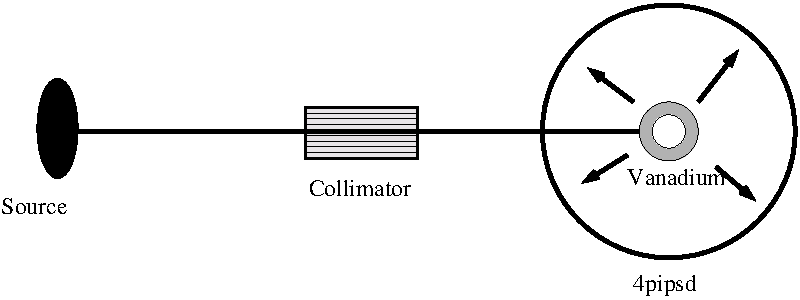
\includegraphics[width=0.9\textwidth]{figures/vanadium}
  \end{center}
\caption{A sketch of the test instrument for the component
V\_sample.}
\label{f:V-instr}
\end{figure}

\subsection{Scattering from the V-sample test instrument}
\label{s:vanadium-result}

In figure \ref{f:V-results}, we present the radial distribution
of the scatting from an evenly illuminated V-sample,
as seen by a spherical PSD.
It is interesting to note that the variation in the
scattering intensity is as large as 10\%. This is an effect
of anisotropic attenuation of the beam in the cylindrical sample.

\begin{figure}
  \begin{center}
    \includegraphics[width=0.6\textwidth]{figures/vanadium-surf-2.eps}
  \end{center}
\caption{Scattering from a V-sample, measured by a spherical
  PSD. The sphere has been transformed onto a plane and the intensity is
  plotted as the third dimension. }
\label{f:V-results}
\end{figure}



\section{The triple axis spectrometer TAS1}
\label{s:TAS1}
With this instrument definition, we have tried to create
a very detailed model of the conventional cold-source
triple-axis spectrometer TAS1 at the now closed neutron source DR3 of
Ris\o\ National Laboratory.
Except for the cold source itself, all components
used have quite realistic properties. Furthermore, the overall
geometry of the instrument has been adapted from
the detailed technical drawings of the real spectrometer.
The TAS 1 simulation was the first detailed work
performed with the \MCS\ package.
For further details see reference~\cite{tas1_report}.

At the spectrometer, the channel from the cold source
to the monochromator is asymmetric, since the first
part of the channel is shared with other instruments.
In the instrument definition, this is represented by
three slits.
For the cold source, we use a flat energy
distribution (component {\bf Source\_flat})
focusing on the third slit.

The real monochromator consist of seven blades, vertically focusing on
the sample. The angle of curvature is constant so that the focusing is
perfect at 5.0 meV (20.0 meV for 2nd order reflections) for a 1$\times$1~cm$^2$
sample. This is modeled directly in the instrument definition using
seven {\bf Monochromator} components. The mosaicity of the pyrolytic
graphite crystals is nominally 30' (FWHM) in both directions.  However, the
simulations indicated that the horisontal mosaicities of both
monochromator and analyser were more likely 45'. This was used for all
mosaicities in the final instrument definition.

The monochromator scattering angle, in effect determining the incoming
neutron energy, is for the real spectrometer fixed by four holes in the
shielding, corresponding to the energies 3.6, 5.0, 7.2, and 13.7~meV for
first order neutrons.  In the instrument definition, we have adapted the
angle corresponding to 5.0~meV in order to test the simulations against
measurements performed on the spectrometer.

The width of the exit channel from the monochromator may
be narrowed down from initially 40~mm
to 20~mm by an insert piece. In the simulations, we have chosen
the 20~mm option and modeled the channel with two slits to match
the experimental set-up.

In the test experiments, we used two standard samples:
An Al$_2$O$_3$ powder sample and a vanadium sample. The instrument
definitions use either of these samples of the correct
size. Both samples are chosen to focus on the opening aperture of
collimator 2 (the one between the sample and the analyser).
Two slits, one before and one after the sample,
are in the instrument definition set to the opening values which
were used in the experiments.

The analyser of the spectrometer is flat and made from
pyrolytic graphite. It is placed between an entry and
an exit channel, the latter leading to a single detector.
All this has been copied into the instrument definition.

On the spectrometer, Soller collimators may be inserted
at three positions: Between monochromator and sample,
between sample and analyser, and between analyser and detector.
In our instrument definition, we have used 30', 28', and 67' collimators
on these three positions, respectively.

An illustration of the TAS1 instrument
is shown in figure~\ref{f:TAS1}.
Test results and data from the real spectrometer are shown
in Appendix~\ref{data:TAS1}.

\begin{figure}
  \begin{center}
    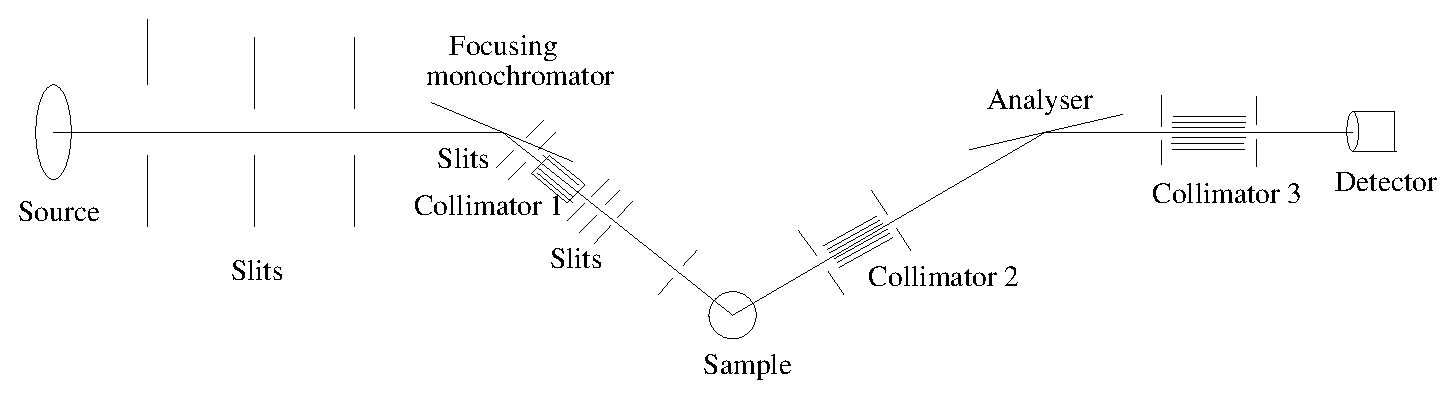
\includegraphics[width=0.9\textwidth]{figures/tas1.eps}
  \end{center}
\caption{A sketch of the TAS1 instrument.}
\label{f:TAS1}
\end{figure}

\subsection{Simulated and measured resolution of TAS1}
\label{data:TAS1}

In order to test the \MCS\ package on a qualitative level,
we have performed a very detailed comparison of a simulation with a
standard experiment from TAS1. The measurement series
constitutes a complete alignment of the spectrometer,
using the direct beam and scattering from V and Al$_2$O$_3$
samples at an incoming energy of 20.0~meV, using the second order
scattering from the monochromator.

In these simulations, we have tried to reproduce
every alignment scan with respect to position and width
of the peaks, whereas we have not tried to compare
absolute intensities. Below, we show a few comparisons
of the simulations and the measurements.

Figure \ref{f:2t_direct} shows a scan of
$2\theta_m$ on the collimated direct beam in two-axis mode.
A \hbox{1 mm} slit is placed on the sample position.
Both the measured width and non-Gaussian peak shape
are well reproduced by the \MCS\ simulations.

\begin{figure}
  \begin{center}
    \includegraphics[width=0.6\textwidth]{figures/tas1-2T.eps}
  \end{center}
\caption{TAS1: Scans of $2\theta_s$ in the direct beam with 1 mm slit on the
  sample position.
"$\times$": measurements, "o": simulations, scaled to the same intensity
Collimations: open-30'-open-open.}
\label{f:2t_direct}
\end{figure}

In contrast, a simulated $2\theta_a$ scan in triple-axis
mode on a V-sample showed a surprising offset from 0 degrees.
However, a simulation with a PSD
on the sample position showed that the beam center was 1.5~mm
off from the center of the sample, and this was important
since the beam was no wider than the sample itself.
A subsequent centering of the beam resulted in a nice
agreement between simulation and measurements.
For a comparison on a slightly different instrument
(analyser-detector collimator inserted),
see Figure~\ref{f:v_2ta_zero}.

%\begin{figure}
%  \begin{center}
%    \includegraphics[width=0.6\textwidth]{figures/vanadium-plot-1.eps}
%  \end{center}
%\caption{First simulated $2\theta_a$ scan on a vanadium sample.
%Collimations: open-30'-28'-open.}
%\label{f:v_2ta_offset}
%\end{figure}

\begin{figure}
  \begin{center}
    \includegraphics[width=0.6\textwidth]{figures/vanadium-plot-2.eps}
  \end{center}
\caption{TAS1: Corrected $2\theta_a$ scan on a V-sample.
Collimations: open-30'-28'-67'.
"$\times$": measurements, "o": simulations.}
\label{f:v_2ta_zero}
\end{figure}

The result of a $2\theta_s$ scan on an Al$_2$O$_3$
powder sample in two-axis mode is shown in Figure \ref{f:al2o3}.
Both for the scan in focusing mode (+ $-$ +)
and for the one in defocusing mode (+ + +) (not shown),
the agreement between simulation and experiment is excellent.

\begin{figure}
  \begin{center}
    \includegraphics[width=0.6\textwidth]{figures/al2o3-focus.eps}
  \end{center}
\caption{TAS1: $2\theta_s$ scans on Al$_2$O$_3$ in two-axis, focusing mode.
Collimations: open-30'-28'-67'.
"$\times$": measurements, "o": simulations.
A constant background is added to the simulated data.}
\label{f:al2o3}
\end{figure}

As a final result, we present a scan of the energy
transfer $E_a = \hbar \omega$ on a V-sample.
The data are shown in Figure \ref{f:v_ea}.

\begin{figure}
  \begin{center}
    \includegraphics[width=0.6\textwidth]{figures/ea-scan.eps}
  \end{center}
\caption{TAS1: Scans of the analyser energy on a V-sample.
Collimations: open-30'-28'-67'.
"$\times$": measurements, "o": simulations.}
\label{f:v_ea}
\end{figure}


\section{The time-of-flight spectrometer PRISMA}
\label{s:PRISMA}

In order to test the time-of-flight aspect of \MCS, we have
in collaboration with Mark Hagen, now at SNS, written a simple
simulation of a time-of-flight instrument loosely based on the ISIS
spectrometer PRISMA. The simulation was used to investigate the effect
of using a RITA-style analyser instead of the normal PRISMA backend.

We have used the simple time-of-flight source {\bf Tof\_source}.
The neutrons pass through a
beam channel and scatter off from a vanadium sample, pass through
a collimator on to the analyser.
The RITA-style analyser consists of seven analyser crystals
that can be rotated independently around a vertical axis. After the
analysers we have placed a PSD and a time-of-flight detector.

To illustrate some of the things that can be done in a simulation as
opposed to a real-life experiment, this example instrument further
discriminates between
the scattering off each individual analyser crystal
when the neutron hits the detector. The
analyser component is modified so that a global variable
\verb+neu_color+ registers which
crystal scatters the neutron ray. The detector component
is then modified to construct seven different time-of-flight histograms,
one for each crystal (see the source code for the instrument
for details). One way to think of this is that
the analyser blades paint a color on each neutron which is then
observed in the detector.
An illustration of the instrument is shown in figure~\ref{f:PRISMA}.
Test results are shown in Appendix~\ref{data:PRISMA}.

\begin{figure}[h]
  \begin{center}
    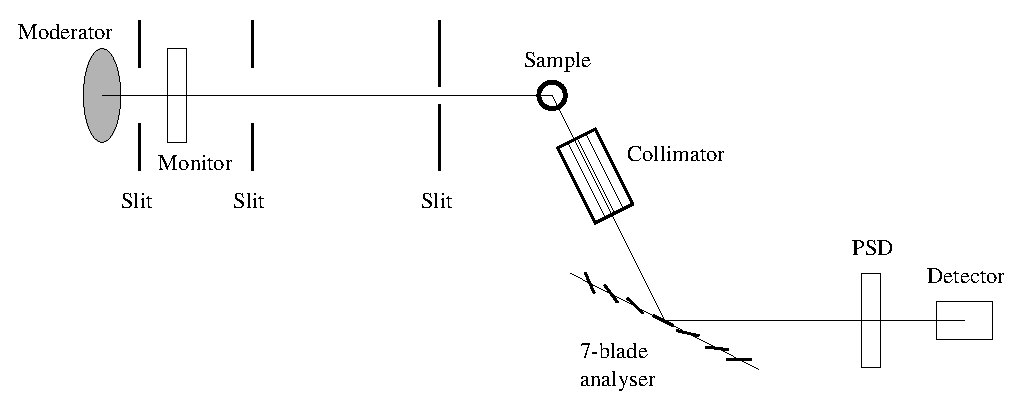
\includegraphics[width=0.9\textwidth]{figures/prisma2.eps}
  \end{center}
\caption{A sketch of the PRISMA instrument.}
\label{f:PRISMA}
\end{figure}

\subsection{Simple spectra from the PRISMA instrument}
\label{data:PRISMA}

A plot from the detector in the PRISMA simulation is shown in Figure
\ref{f:PRISMAdata}. These results were obtained with each analyser blade
rotated one degree relative to the previous one. The separation of the
spectra of the different analyser blades is caused by different energy
of scattered neutrons and different flight path length from source to
detector.  We have not performed any quantitative analysis of the data.

\begin{figure}
  \begin{center}
    \includegraphics[width=0.6\textwidth]{figures/prisma2-a.eps}
  \end{center}
\caption{Test result from PRISMA instrument using ``colored
  neutrons''. Each graph shows the neutrons scattered from one analyser blade.}
\label{f:PRISMAdata}
\end{figure}

%% Emacs settings: -*-mode: latex; TeX-master: "manual.tex"; -*-

\chapter{Test results}
\label{testresults}

In this Appendix, we present a few illustrative
results from the three instruments presented in 
section \ref{s:instrument}. A more thorough presentation
may be found on the \MCS\ home page \cite{mcstas_webpage}.

\section{Scattering from the V-sample test instrument}
\label{s:vanadium-result}

In figure \ref{f:V-results}, we present the radial distribution 
of the scatting from an evenly illuminated V-sample,
as seen by a spherical PSD.
It is interesting to note that the variation in the
scattering intensity is as large as 10\%. This is an effect
of attenuation of the beam in the cylindrical sample.

\begin{figure}
  \begin{center}
    \includegraphics[width=0.6\textwidth]{vanadium-surf-2.eps}
  \end{center}
\caption{Scattering from a V-sample, measured by a spherical
  PSD. The sphere has been transformed onto a plane and the intensity is
  plotted as the third dimension. A colour version of this picture is
  found on the title page of this manual.}
\label{f:V-results}
\end{figure}

\section{Simulated and measured resolution of TAS1}
\label{data:TAS1}

In order to test the \MCS\ package on a qualitative level,
we have performed a very detailed simulation of the conventional
triple axis spectrometer TAS1, Ris\o . The measurement series
constitutes a complete alignment of the spectrometer,
using the direct beam and scattering from V and Al$_2$O$_3$
samples at an incoming energy of 20.0~meV, using the second order
scattering from the monochromator. 
In the instrument definitions, we have used all available
information about the spectrometer. However, the
mosaicities of the monochromator and analyser are set
to 45' in stead of the quoted 30', since we from our
analysis believe this to be much closer to the truth.

In these simulations, we have tried to reproduce
every alignment scan with respect to position and width
of the peaks, whereas we have not tried to compare
absolute intensities. Below, we show a few comparisons 
of the simulations and the measurements. 

Figure \ref{f:2t_direct} shows a scan of 
$2\theta_s$ on the collimated direct beam in two-axis mode.
A 1 mm slit is placed on the sample position.
Both the measured width and non-Gaussian peak shape
are well reproduced by the \MCS\ simulations.

\begin{figure}
  \begin{center}
    \includegraphics[width=0.6\textwidth]{tas1-2T.eps}
  \end{center}
\caption{Scans of $2\theta_s$ in the direct beam with 1 mm slit on the
  sample position.
"$\times$": measurements, "o": simulations  
Collimations: open-30'-open-open.}
\label{f:2t_direct}
\end{figure}

In contrast, a simulated $2\theta_a$ scan in triple-axis 
mode on a V-sample showed a surprising offset from zero, see
Figure \ref{f:v_2ta_offset}. However, a simulation with a PSD
on the sample position showed that the beam center was 1.5~mm
off from the center of the sample, and this was important
since the beam was no wider than the sample itself.
A subsequent centering of the beam resulted in a nice
agreement between simulation and measurements. 
For a comparison on a slightly different instrument
(analyser-detector collimator inserted), 
see Figure~\ref{f:v_2ta_zero}.

\begin{figure}
  \begin{center}
    \includegraphics[width=0.6\textwidth]{vanadium-plot-1.eps}
  \end{center}
\caption{First simulated $2\theta_a$ scan on a vanadium sample.
Collimations: open-30'-28'-open.}
\label{f:v_2ta_offset}
\end{figure}

\begin{figure}
  \begin{center}
    \includegraphics[width=0.6\textwidth]{vanadium-plot-2.eps}
  \end{center}
\caption{Corrected $2\theta_a$ scan on a V-sample.
Collimations: open-30'-28'-67'.
"$\times$": measurements, "o": simulations.}
\label{f:v_2ta_zero}
\end{figure}

The result of a $2\theta_s$ scan on an Al$_2$O$_3$
powder sample in two-axis mode is shown in Figure \ref{f:al2o3}.
Both for the scan in focusing mode (+ $-$ +)
and for the one in defocusing mode (+ + +) (not shown),
the agreement between simulation and experiment is excellent.

\begin{figure}
  \begin{center}
    \includegraphics[width=0.6\textwidth]{al2o3-focus.eps}
  \end{center}
\caption{$2\theta_s$ scans on Al$_2$O$_3$ in two-axis, focusing mode.
Collimations: open-30'-28'-67'.
"$\times$": measurements, "o": simulations.  
A constant background is added to the simulated data.}
\label{f:al2o3}
\end{figure}

As a final result, we present a scan of the energy
transfer $E_a = \hbar \omega$ on a V-sample.
The data are shown in Figure \ref{f:v_ea}.

\begin{figure}
  \begin{center}
    \includegraphics[width=0.6\textwidth]{ea-scan.eps}
  \end{center}
\caption{Scans of the analyser energy on a V-sample.
Collimations: open-30'-28'-67'.
"$\times$": measurements, "o": simulations.}
\label{f:v_ea}
\end{figure}


\section{Simple spectra from the PRISMA instrument}
\label{data:PRISMA}

A plot from the detector in the PRISMA simulation is shown in Figure
\ref{f:PRISMAdata}. These results were obtained with each analyser blade
rotated one degree relative to the previous one. The separation of the
spectra of the different analyser blades is caused by different energy
of scattered neutrons and different flight path length from source to
detector.  We have not performed any quantitative analysis of the data at this
time.

\begin{figure}
  \begin{center}
    \includegraphics[width=0.6\textwidth]{prisma2-a.eps}
  \end{center}
\caption{Test result from PRISMA instrument using ``coloured
  neutrons''. Each graph shows the neutrons scattered from one analyser blade.}
\label{f:PRISMAdata}
\end{figure}

   % now in instrum
%% Emacs settings: -*-mode: latex; TeX-master: "manual.tex"; -*-

\chapter{Planned expansions of \MCS\ in the future}
\label{future}

During the work so far on
\MCS, we have run across a number of points we would like to
include in \MCS\ in the future.

For the \MCS\ meta-language itself, these points include:
\begin{itemize}
\item Facilities for making a Monte-Carlo choice on the basis of 
tabulated values. This would be useful in source and filter components.
\item Facilities for assembling a number of existing components into one
compound component, like a multi-bladed analyser.
\end{itemize}
We also would like to improve on the component and instrument libraries:
\begin{itemize}
\item Output in NeXus format.
\item Allow multiple scattering in sample components.
\item More samples for inelastic scattering.
\item A powder sample with more than one reflection.
\item Handle gravitation.
\item The RITA spectrometer.
\item The new Ris\o\ TAS7 spectrometer.
\item A detailed version of the ISIS PRISMA spectrometer.
\end{itemize}
Further, we would like to make improvements on the interface software:
\begin{itemize}
\item Interface to existing control software ({\em e.g.} the Ris\o{}
  program TASCOM)
\end{itemize}
 % now in changes

\appendix
%% Loads of preamble stripped off - now located in mcstas.tex

%\newpage
\chapter{Polarization in McStas}
\label{c:polarization}
\begin{center}
\Large{P. Christiansen (Ris{\o})\\\today}
\end{center}

\section{Introduction}

In the current release of McStas there are components with polarization
capabilities. At the moment all such components should be understood as under
development as the amount of testing and debugging of these components is
small, and there are known problems. 

Here, we shall report on what have been done so far.

We first describe the polarization vector and how it is related to the neutron
wave-function (section~\ref{sec:pol}) and then the physics of simple
components that we need in McStas is reviewed (section~\ref{sec:scat}). In the
last two sections the actual McStas polarization components are first
described (section~\ref{sec:new}) and a list of test instruments in McStas is
given (section~\ref{sec:test}).

We rely heavily on the books~\cite{lovesey,gavin} for the physics where
the detailed calculations can be found. 

The notation used here (and in~\cite{gavin}) is $P$ (scalar), $\PB$
(vector), $\tP$ (unit-vector), $\sigmaH$ (operator), and $\sigmao$
(vector of operators).

\section{The Polarization Vector}
\label{sec:pol}

The spin of the neutron is represented by an operator $\so$ for which only a
single component can be measured at one time. Each single measurement will
give a value $\pm 1/2$, but if we could make a large number of measurements on
the same neutron state, in each of the three axis directions, and then make
the average we get $\langle \so \rangle$. The polarization vector, $\PB$, is
then defined as:
\begin{equation}
  \label{eq:pol_single}
  \PB = \frac{\langle \so \rangle}{s},
\end{equation}
so that $-1 \leq |\PB| \leq +1$

For a neutron beam which contains $N$ neutrons, each with a
polarization $\PB_i$, the beam polarization is defined as:
\begin{equation}
  \label{eq:pol_beam}
  \PB = \frac{\sum_i \PB_i}{N}.
\end{equation}

If we have one common quantization direction (e.g. a magnetic field
direction) each neutron will either be spin up, $\uparrow$, or spin down,
$\downarrow$, and the polarization can be expressed as:

\begin{equation}
  \label{eq:pol}
  P = \frac{\nu-\nd}{\nu+\nd},
\end{equation}

where $\nu$ ($\nd$) is the number of neutrons with spin up
(down).

For a given neutron the probability of the neutron being spin up, $\Pu$, is: 

\begin{equation}
  \label{eq:prob_spinup}
  \Pu = \frac{\nu}{\nu+\nd} = \frac{\nu + (\nd-\nd)/2}{\nu+\nd} 
  = \frac{1+P}{2},
\end{equation}

and $\Pd = 1-\Pu = (1-P)/2$. 

The expectation value of the 'spin' operator, $\sigmao$, which can be
expressed by the Pauli matrices, is the polarization vector $\PB$, $\PB =
\langle \sigmao \rangle \equiv \langle \chi | \sigmao | \chi \rangle$.  The
most general form of the spin wave-function $\chi$ for a neutron (spin 1/2)
is:

\begin{equation}
  \label{eq:neutron_wave}
  \chi = a\chi_\uparrow + b\chi_\downarrow,
\end{equation}

where $\chi_\uparrow$ and $\chi_\downarrow$ are eigenfunction of
$\hat{\sigma}^z$, and the complex coefficients $a$ and $b$ satisfy
$|a|^2 + |b|^2 = 1$.

By calculation we find:
\begin{eqnarray}
P_x & = & \langle \chi | \sigmaH_x | \chi \rangle
= 2 \text{Re}(a^\ast b) \\
P_y & = & \langle \chi | \sigmaH_y | \chi \rangle
= 2 \text{Im}(a^\ast b) \\
P_z & = & \langle \chi | \sigmaH_z | \chi \rangle
= |a|^2-|b|^2
\end{eqnarray}

This shows the relation of the polarization vector to the neutron wave
function. 

The neutron magnetic moment operator can be expressed in terms of $\sigmao$,
as:
\begin{equation}
  \label{eq:magnetic}
  \muno = \mu_n \sigmao,
\end{equation}
which, as shown above, is related to the polarization vector.  \\

In our simulation we represent the polarization by the vector $\SB = (s_x,
s_y, s_z)$ which is propagated through the different components so it has the
correct relative orientation in each component. The probability for the spin
to be parallel a given direction $\mathbf{n}$ is then:

 \begin{equation}
   \label{eq:probmcstas}
   P(\uparrow|\nB) = \frac{1+\nB \cdot \SB}{2}.
 \end{equation}

This equation (from~\cite{pol_seeger}) is easy to understand. The
average spin along $\nB$ is $\nB \cdot \SB$ and the probability then
follows from Eq.~\ref{eq:prob_spinup}.

For an unpolarized beam, $\mathbf{S} = \mathbf{0}$ and all directions
are equally probable (50~\%).

Note that in our approach we do not decide if the neutron is up or down after
a given component, but instead keep track of as much information for as long
as possible.

In the following we will use $\PB$ to denote the polarization
vector. The most important variables used are:

\begin{tabular}{ll}
    
  $\Q$  & Scattering vector. \\
  $\PB$  & Polarization before a component (ingoing). \\ 
  $\PB_\perp$  & Polarization perpendicular to scattering vector, 
  $\PB_\perp = \tQ \times (\PB \times \tQ$). \\ 
  $\PB'$ & Polarization after a component (outgoing). \\
  $\tN$ & Unit vector in direction of atomic spin ($\tN \cdot \tilde{\BB} = -1$ for a ferromagnet). \\
  $\FN$ & Unit cell nuclear structure factor. \\
  $\FM$ & Unit cell magnetic structure factor. \\
\end{tabular}
\\

The unit cell nuclear structure factor is defined as:

\begin{equation}
  \FN = \sum_\dB
  \exp(i\Q \cdot \dB)\overline{b}_d,
\end{equation}

where the $\dB$ is the position of the d'th atom within the unit cell,
and $\overline{b}_d$ is the average of $b_d$. In the simple case of a
single atom Bravais crystal one finds $\FN = \overline{b}$.

The unit cell magnetic structure factor is useful when the atoms in
the crystal only have spin orbital angular momentum, and simple when
the magnet is saturated (all spins are parallel or anti-parallel to
\emph{one} direction, $\sigma_d=\pm1$). It is then given as: 

\begin{equation}
  \FM =
  \gamma_n r_0 \sum_\dB \exp(i\Q \cdot \dB)\frac{1}{2}g_d F_d(\Q)\langle
  \hat{S}_d\rangle \sigma_d,
\end{equation}

where $r_0=\frac{\mu_0}{4\pi}\frac{e^2}{m_e} = 2.818 \times 10^{-15}$m, $g=2$ is the
Land{\'e} splitting factor, and $F_d(\Q)$ is the magnetic form factor, which
is the Fourier transform of the magnetization density (normalized so that
$F_d(0) = 1$), and $\langle \hat{S}_d\rangle$ is the thermal average of the
ordered atomic spin.

In the following the Debye-Weller factor ($\exp(-W_d)$) have been ignored in
all cross sections.

\subsection{Example: Magnetic fields}

The magnetic moment operator of the neutron is $\muno = \gamma_n \so$, where
$\gamma_n = 2 \mu_n = -3.826$ is the gyromagnetic ratio (spin and magnetic
moment is anti-parallel as for an electron)~\footnote{Note that if we had used
S (with values $S=\pm 1$) to define $\gamma_n$ we would get $\gamma_n =
-1.913$ which is also commonly used.}

A magnetic field, $\BB$, will exert a torque, $\tauB = d\sB/dt = (1/\gamma_n)d\muB/dt$, on the neutron magnetic moment:
 
\begin{equation}
  \label{eq:torque}
  \frac{1}{\gamma_n} \frac{d\muB}{dt} = \muB \times \BB
\end{equation}
 
The magnetic moment $\mu$ can be related to the polarization as $\muB
= \gamma_n \PB/2$, and inserting in Eq.~\ref{eq:torque} we find:

\begin{equation}
  \label{eq:pol_magnetic}
  \frac{d\PB}{dt} = \gamma_n \PB \times \BB
\end{equation}

In the simple case where $\BB = (0, 0, B)$, we find the solution
(\cite{gavin} p.~18) :

\begin{eqnarray}
  \nonumber
  P_X(t) & = & \cos(\omega_L t) P_X(0) - \sin(\omega_L t) P_Y(0) \\
  \label{eq:precession}
  P_Y(t) & = & \sin(\omega_L t) P_X(0) + \cos(\omega_L t) P_Y(0) \\
  \nonumber
  P_Z(t) & = & P_Z(0),
\end{eqnarray}

where $\omega_L = -\gamma_n B/\hbar$ is the Larmor frequency.\\

\begin{quote}
  The equations above was checked against the equations in the ``polarimetrie
  neutronique'' notes by Francis Tasset and found to be consistent. There can
  be sign differences between different publications depending on whether they
  use a right-handed (like e.g. McStas) or a left-handed (like e.g. NISP)
  coordinate system.
\end{quote}

\section{Polarized Neutron Scattering}
\label{sec:scat}

First we will give a short introduction to how calculations are done
and then quote some results which are important for implementing the
first McStas components.

All the potentials (nuclear, magnetic, and electric) we will be interested in
can be written on the form:
\begin{equation}
  \label{eq:general_pot}
  \hat{v} = \betao + \alphao \cdot \sigmao
\end{equation}

The first term does not affect the spin, while the second term can
change the spin. Let us just remind here that:

\begin{equation}
  \label{eq:pauli_rules}
  \begin{matrix}
    \sigmaH_x \chiU = \chiD, &
    \sigmaH_y \chiU = i\chiD, &
    \sigmaH_z \chiU = \chiU, \\
    \sigmaH_x \chiD = \chiU, &
    \sigmaH_y \chiD = -i\chiU, &
    \sigmaH_z \chiD = -\chiD.
  \end{matrix} 
\end{equation}

So that the interaction proportional to $\sigmaH_x$ and $\sigmaH_y$
results in spin flips, while the interactions with $\sigmaH_z$
conserves the spin.

It turns out to be smart to define a density matrix operator:
\begin{equation}
  \rhoo = \chi \chi^\dagger =  
  \left( \begin{matrix} 
    |a|^2 & ab^\ast \\ 
    ba^\ast & |b|^2 
  \end{matrix} \right) 
  = \frac{1}{2}({\cal I}+\PB \cdot \sigmao),
\end{equation}
where $\chi$ is the neutron wave function (Eq.~\ref{eq:neutron_wave}),
and ${\cal I}$ is the unit matrix.

Using the density matrix the elastic cross section can be written as
(\cite{lovesey}, Eq.~10.31):
\begin{equation}
  \label{eq:master_sigma}
  \frac{d\sigma}{d\Omega} = \text{Tr} \rhoo \hat{v}^\dagger \hat{v}
  = \sum_{\lambda, \lambda'} p_\lambda \text{Tr} \rhoo
  \langle \lambda | \hat{V}^\dagger(\Q) | \lambda' \rangle
  \langle \lambda' | \hat{V}(\Q) | \lambda \rangle
  \delta(E_\lambda - E_{\lambda'}),
\end{equation}

where $\hat{V}$ is the interaction potential and it is understood that
the trace is to be taken with respect only to the neutron spin
coordinates. The outgoing polarization is given as:
\begin{equation}
  \label{eq:master_pol}
  \PB' \frac{d\sigma}{d\Omega} = 
  \text{Tr} \rhoo \hat{v}^\dagger \sigmao \hat{v}
  = \sum_{\lambda, \lambda'} p_\lambda \text{Tr} \rhoo
  \langle \lambda | \hat{V}^\dagger(\Q) | \lambda' \rangle
  \sigmao
  \langle \lambda' | \hat{V}(\Q) | \lambda \rangle
  \delta(E_\lambda - E_{\lambda'}) 
\end{equation}

Inserting Eq.~\ref{eq:general_pot} in Eq.~\ref{eq:master_sigma} and
Eq.~\ref{eq:master_pol} results in the two master equations for
polarized neutron scattering:

\begin{equation}
  \label{eq:general_sigma}
  \text{Tr} \rhoo \hat{v}^\dagger \hat{v} = 
  \alphao^\dagger \cdot \alphao + \betao^\dagger \betao+
  \betao^\dagger (\alphao \cdot \PB) +
  (\alphao^\dagger \cdot \PB) \betao +
  i\PB \cdot (\alphao^\dagger \times \alphao),
\end{equation}

and 

\begin{equation}
  \label{eq:general_pol}
  \text{Tr} \rhoo \hat{v}^\dagger \sigmao \hat{v} =
  \betao^\dagger \alphao
  + \alphao^\dagger \betao
  + \betao^\dagger \betao \PB 
  + \alphao^\dagger (\alphao \cdot \PB) 
  + (\alphao^\dagger \cdot \PB) \alphao 
  - \PB (\alphao^\dagger \cdot \alphao)
  - i \alphao^\dagger \times \alphao
  + i \betao^\dagger (\alphao \times \PB)
  + i (\PB \times \alphao^\dagger) \betao.
\end{equation}

Based on these two equations and the interaction potentials all the
results presented in the following are derived in~\cite{lovesey}.

\subsection{Example: Nuclear scattering}

The nuclear scattering potential for a crystal is:
\begin{equation}
  \label{eq:nuclear_pot}
  \hat{V}_N(\Q) = \sum_{\lB,\dB} \exp(i\Q \cdot \RB_{ld})(A_{ld} + 
  \frac{1}{2} B_{ld} \sigmao \cdot \Io_{ld}),
\end{equation}

so that 

\begin{eqnarray}
  \label{eq:ab_nuclear}
  \alphao & = & 
  \sum_{\lB,\dB} \exp(i\Q \cdot \RB_{ld}) \frac{1}{2} B_{ld} \Io_{ld} \\
  \betao & = &
  \sum_{\lB,\dB} \exp(i\Q \cdot \RB_{ld}) A_{ld},
\end{eqnarray}

where $\Io$ is the nuclear spin operator and the constants $A$ and $B$
are related to the nuclear scattering lengths $b^+$ and $b^-$ as
$A=((I+1)b^++Ib^-)/(2I+1)$ and $B=(b^++b^-)/(2I+1)$.

To calculate the polarization cross section and outgoing polarization
we have to average over the nuclear spin (which we assume is random
oriented), so that terms linear in $\alphao$ (three last terms in
Eq.~\ref{eq:general_sigma}) disappears. The scattering cross section
ends up being (see~\cite{lovesey} p.~159):

\begin{equation}
  \label{eq:nuclear_sigma}
  \frac{d\sigma}{d\Omega}  = 
  \sum_{\lB, \dB, \lB', \dB'} \exp(i \Q \cdot (\RB_{ld}-\RB_{l'd'}))
  (\madsq + \delta_{\lB,\lB'}\delta_{\dB,\dB'}[\sqmad - \madsq 
  + \frac{1}{4}\bd])
\end{equation}

where the first term is the coherent cross-section and the second term is the
site-incoherent cross-section. Both terms are independent of $\PB$ as expected
for a system without a preferred internal direction.

The polarization in the final state is:

\begin{equation}
  \label{eq:nuclear_pol}
  \PB' \frac{d\sigma}{d\Omega}  = 
  \sum_{\lB, \dB, \lB', \dB'} \exp(i \Q \cdot (\RB_{ld}-\RB_{l'd'}))
  \PB' (\madsq + \delta_{\lB,\lB'}\delta_{\dB,\dB'}[\sqmad - \madsq
  - \frac{1}{12}\bd])
\end{equation}

Comparing Eq.~\ref{eq:nuclear_sigma} and Eq.~\ref{eq:nuclear_pol} we
find that: 1) The nuclear coherent polarization is the same as the
initial polarization. 2) The same is true for the incoherent
scattering due to the random isotope distribution. 3) The nuclear
incoherent scattering due to the random nuclear spin orientations has
polarization $\PB' = -1/3 \PB$ (for a random nuclear spin the
associated Pauli matrix will 2/3 of the time point in the direction of
$\sigmaH_x$ and $\sigmaH_y$ which according to
Eq.~\ref{eq:pauli_rules} flips the spin). \\

For Vanadium, where there is only one isotope and coherent scattering
is negligible, we find $\PB' = -1/3\PB$. There is however one
catch. If the probability for multiple scattering is large one has to
take into account that after two scattering one has: $\PB'(2) =
1/9\PB$, and so forth. The average polarization after a thick vanadium
target is therefore a sum of different contributions.

\subsection{Example: Polarizing Monochromator and Guides}
\label{sub:mono}

\begin{figure}[htbp]
  \begin{center}
    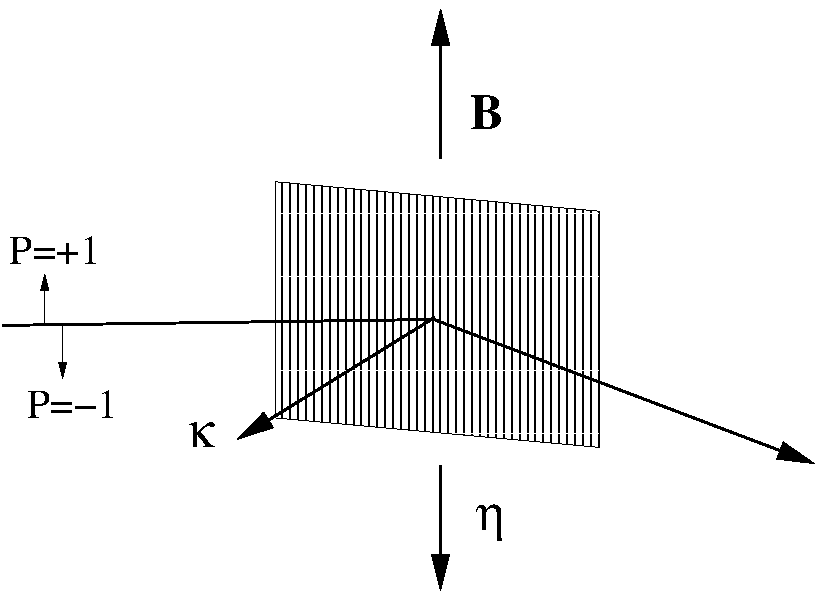
\includegraphics[keepaspectratio,
    width=0.7\columnwidth]{figures/monochromator_pol}
    \caption{Principle and geometry of a polarizing monochromator.}
    \label{fig:mono_princip}
  \end{center}
\end{figure}

In a polarized monochromator and polarizing guides we have a ferromagnetic
crystal in an external magnetic field. The scattering potential is now both
nuclear (no internal direction) and magnetic (internal direction), so in
general the outgoing polarization can be quite complex. However, as
illustrated in Figure~\ref{fig:mono_princip}, the typical setup has many
geometrical constraints: $\tN \cdot \tQ = 0$, $\tN \cdot \PB_\perp = \tN \cdot
\PB$, and $\Q \times (\tN \times \Q) = \tN$, which simplifies the problem.

In~\cite{lovesey} the calculation for a centrosymmetric ferromagnetic
crystal is done, and inserting the constraints above one finds
(\cite{lovesey84}, Eq.~10.96 and Eq.~10.110):

\begin{eqnarray}
  \label{eq:mono_sigma}
  d\sigma/d\Omega & = & \FN^2 + 2\FN\FM (\PB \cdot \tN) + \FM^2\\
  \label{eq:mono_pol}
  \PB' d\sigma/d\Omega & = 
  & \PB [\FN^2 - \FM^2] + \tN [2\FN\FM + 2(\tN \cdot \PB)\FM^2]
\end{eqnarray}

\begin{quote}
  NB! Note that in~\cite{gavin} Eq.~2.2.25 there is a minus in front of the
  second term in Eq.~\ref{eq:mono_sigma}. We have not been able to understand
  this discrepancy, which is probably due to notation. Most other authors
  agree with the minus in front of the second term (e.g. Squires and Francis
  Tasset).
\end{quote}

For a beam which is initially unpolarized we find the outgoing
polarization to be:
\begin{equation}
  \PB' = \frac{\tN 2\FN \FM}{d\sigma/d\Omega} 
  = \frac{2\FN\FM}{\FN^2 + \FM^2} \tN,
\end{equation}

so that the beam is fully polarized along $\tN$ if $\FN = \pm \FM$. \\

What we use to characterize the polarizing monochromator in practice
is not $\FN$ and $\FM$, but instead the reflection probabilities $\Ru$
and $\Rd$ (for the reflection of interest).

If we assume that the reflection probabilities are directly proportional to
the cross sections (with proportionality constant $k$), i.e., $\Ru = k
d\sigma/d\Omega(\PB=+\tN)$ and $\Rd = k d\sigma/d\Omega(\PB=-\tN)$ then we can
use Eq.~\ref{eq:mono_sigma} to determine $\FN$ and $\FM$:

\begin{eqnarray}
  \label{eq:mono_up}
  \Ru & = & k (\FN + \FM)^2,\\
  \label{eq:mono_down}
  \Rd & = & k (\FN - \FM)^2.
\end{eqnarray}

The values of $\sqrt{k}\FN$ and $\sqrt{k}\FM$ are then between -1 and +1 and
unit less like the reflection probabilities. In the following we ignore $k$ and
just talk about $\FN$ and $\FM$.

In principle there are four solutions for $\FN$ and $\FM$, so in the code we
currently choose the values where $\FN + \FM = +\sqrt{\Ru}$ and $\FN - \FM =
+\sqrt{\Rd}$ (so that $\FN>0$ and $\FN>\FM$). We then find:

\begin{eqnarray}
  \label{eq:mono_nuc}
  \FN & = & \frac{\sqrt{\Ru} + \sqrt{\Rd}}{2},\\
  \label{eq:mono_mag}
  \FM & = & \frac{\sqrt{\Ru} - \sqrt{\Rd}}{2}.
\end{eqnarray}

When $\FN$ and $\FM$ are determined from these equations,
Eq.~\ref{eq:mono_sigma} and Eq.~\ref{eq:mono_pol} can easily be used to handle
any situation.

This solution is both used for monochromators and guides.

It is not clear that this solution is correct. If we make a simple example
with $\Ru = 1$ and $\Rd = 0.25$ then we could in principle have four
solutions, but let us just quote the two where $\FN$ is positive since the
last two are found by inserting a minus before all the solutions and this does
not change the physics. The two solutions are $\FN = 0.75, \FM=0.25$ and $\FM
= 0.75, \FN=0.25$. All solutions gives the same cross section, but if the
incoming beam is polarized (and only then) the outgoing beam will have two
different polarization values, since $\PB [\FN^2 - \FM^2]$ and $\tN 2(\tN
\cdot \PB)\FM^2$ are different for the two solutions. It seems that one needs
some additional information to choose between the two solutions.

\begin{quote}
  NB! The simplifying geometry shown in Figure~\ref{fig:mono_princip} only
  applies for the sides of the guide wall and not the top and bottom (assuming
  that the magnetizing field is pointing up or down), so there another set of
  equations should really be used.
\end{quote}

The same physics could also be used for a polarizing powder or single crystal
sample if $\FN$ and $\FM$ can be calculated with some other program, but one
would have to use the general form of Eq.~\ref{eq:mono_sigma} and
Eq.~\ref{eq:mono_pol} without the simplifying geometrical constraints for
monochromators and guides.

\section{New McStas Components}
\label{sec:new}

The components written so far can be divided into four groups:
\begin{itemize}
\item \textbf{Polarizers:} Components used to make the beam polarized.
\item \textbf{Monitors:} Unphysical detectors that can measure the polarization
of the neutrons.
\item \textbf{Magnetic fields:} Components used to handle magnetic fields.
\item \textbf{Samples:} Samples that affects the polarization.
\end{itemize}

\subsection{Polarizers}

Some of the most common ways of polarizing a beam have been
implemented.

\begin{itemize}
\item \textbf{Set\_pol:} This unphysical component can be used in two
ways. Either to hard code the polarization to the vector $(px, py, pz)$
or when randomOn!=0 to set the polarization vector to a random vector
on the unit sphere.\\
  
\item \textbf{Monochromator\_pol:} A monochromator that only does the $n=1$
  reflection. For each neutron it calculates the wavelength which would give
  Bragg reflection, $\lambda_\text{Bragg}$, and it then calculates, based on
  one mosaicity and one d-spread, the reflection probability given the neutrons
  actual $\lambda$.  The reflection probability is a Gaussian in $\Delta
  \lambda = \lambda - \lambda_\text{Bragg}$, with the peak reflectivity and
  polarization calculated as described in section~\ref{sub:mono}.

  \begin{quote}
    NB! Note that this monochromator reflects the neutrons billiard-like. In
    \textbf{Monochromator\_flat} the mosaicity of the reflecting crystal is
    taken into account, but the d-spread is not taken into account. One should
    implement d-spread and mosaicity in a way similar to what is done in
    \textbf{Single crystal}.
  \end{quote}

\item \textbf{Pol\_mirror:} Plane with a reflection probability for up
and down. There are 3 options: always reflect, always transmit, or
random select transmit/reflect. 

\begin{quote}
  NB! Note that at the moment the plane only reflects from one side (because
  it uses PROP\_Z0.
\end{quote}

\item \textbf{Pol\_bender:} Curved guide with the possibilities to
  insert multiple slits, and have the end gap parallel to the entrance
  or following the guide angle. It is possible to select different
  coatings (mirror parameters) for each of the four sides.\\

\item \textbf{Pol\_guide\_vmirror:} Straight guide with non-polarizing
  coatings with two polarizing super mirrors sitting in a V shape
  inside. \\
\end{itemize}

Note that for all the polarizing guides it is possible to define analytical
functions or use tables for the up and down reflectivity descriptions.

\subsection{Detectors}

\begin{itemize}
\item \textbf{Pol\_monitor:} One defines a vector $\mathbf{m} = (mx,
  my, mz)$ for the monitor and measures the projection of the spin
  along this vector i.e. $\mathbf{m} \cdot \mathbf{S}$.\\
  
\item \textbf{PolLambda\_monitor:} Measures the projection of the
  spin along the defined vector $\mathbf{m}$ (see
  \textbf{Pol\_monitor}) as a function of the wavelength $\lambda$.
  
\item \textbf{MeanPolLambda\_monitor:} Measures the \emph{average}
  projection of the spin along the defined vector $\mathbf{m}$ (see
  \textbf{Pol\_monitor}) as a function of the wavelength $\lambda$.

  \begin{quote}
    NB! currently the error on the mean is shown ($\sigma/\sqrt(N)$), but it
    might make more sense to show the spread ($\sigma$).
  \end{quote}
\end{itemize}

\subsection{Magnetic fields}

Much inspiration for the components and the tests have been found
in~\cite{pol_seeger}.

\begin{itemize}
\item \textbf{Pol\_constBfield:} A rectangular box with a constant magnetic
  field in the y-direction. The x- and z-components of the spin precess with
  the Larmor frequency $\omega_L$. It is possible to define the field in terms
  of a wavelength so that the spin will precess 180 degrees for the given
  wavelength. The component can be rotated to have the field along another
  axis. \\
  
\item \textbf{Pol\_simpleBfield:} The first attempt at a component for
  handling general magnetic fields. It is a concentric component where you
  define a start and stop component for each field, but this allows other
  components, e.g. monitors, to be put inside the field. The component
  overloads the propagation routines so that numerical spin propagation is
  done for analytical magnetic fields. 
  
  \begin{quote}
    NB! At the moment both components does not really check the boundaries of
    the field on the sides, but merely assumes that the field starts at the
    entrance plane and stops at the exit plane.

    Also, some optimization remains for the numerical component and it would
    be nice to support tabulated magnetic field files. However, the framework
    developed for \textbf{Pol\_simpleBfield} is very general and should
    easily facilitate these changes.
  \end{quote}

\end{itemize}


\subsection{Samples}

\begin{itemize}
\item \textbf{V\_sample:} Modified the sample so that the scattered
  neutron has $\PB' = -1/3\PB$. Note that this component does not
  handle multiple scattering, so this approach is correct. If the
  components handled multiple scattering the polarization should be
  set to $\PB' = (-1/3)^n\PB$, where $n$ is the number of
  scatterings.\\
\end{itemize}  


\section{Tests With New Components}
\label{sec:test}

All the test instruments can be found in the McStas examples folder
(go to ``Neutron site/tests'' in mcgui). 

There are basically two kind of tests. The first kind of tests shows
that the polarizing component can reproduce the same results as a
similar non-polarizing component:
\begin{itemize} 
\item \textit{Test\_Monochromators.instr} : Intercomparison of
  \textbf{Monochromator\_flat} and \textbf{Monochromator\_pol}. 
\item \textit{Test\_Pol\_Bender\_Vs\_Guide\_Curved.instr} : Intercomparison of
  \textbf{Guide\_curved} and \textbf{Pol\_bender}.
\end{itemize}

The second type of test illustrates the polarizing capabilities of the
component:
\begin{itemize}
\item \textit{Test\_Magnetic\_Constant.instr} : Constant magnetic field. 
\item \textit{Test\_Magnetic\_Majorana.instr} : Linearly decreasing field with
  small transverse component.
\item \textit{Test\_Magnetic\_Rotation.instr} : Rotating magnetic field. 
\item \textit{Test\_Magnetic\_Userdefined.instr} : Example of how to make a
  user defined analytic magnetic field that can also depend on time. 
\item \textit{Test\_Pol\_Bender.instr} : Illustrates beam polarization with
  the \textbf{Pol\_bender}.
\item \textit{Test\_Pol\_Set.instr} : Tests \textbf{Pol\_set}. 
\item \textit{Test\_Pol\_Guide\_Vmirror.instr} : Illustrates beam polarization
  with the \textbf{Pol\_guide\_vmirror}.
\item \textit{Test\_Pol\_Mirror.instr} : Illustrates beam polarization
  with the \textbf{Pol\_mirror}.
\item \textit{Test\_Pol\_TripleAxis.instr} : An example of a triple axis
  spectrometer with polarizing monochromators, a vanadium sample, and a spin
  flipper.
\end{itemize}
    

\chapter{Random numbers in \MCS}
\label{s:random}
\index{Monte Carlo method}

\section{Transformation of random numbers}
In order to perform the Monte Carlo choices, one needs to be able to
pick a random number from a given distribution. However, most
random number generators only give
uniform distributions over a certain interval.
We thus need to be able to transform between probability distributions,
and we here give a short explanation on how to do this.

Assume that we pick a random number, $x$, from a distribution $\phi(x)$.
We are now interested in the shape of the distribution, $\Psi(y)$, of the
transformed $y=f(x)$, assuming $f(x)$ is monotonous.
All random numbers lying in the interval $[x; x+dx]$
are transformed to lie within the interval $[y; y+f'(x)dx]$, so the
resulting distribution must be $\Psi(y) = \phi(x) / f'(x)$.

If the random number generator selects numbers uniformly in the interval
$[0; 1]$, we have $\phi(x) = 1$ (inside the interval; zero outside), and
we reach
\begin{equation}
\Psi(y) = \frac{1}{f'(x)} = \frac{d}{dy} f^{-1}(y) .
\end{equation}
By indefinite integration we reach
\begin{equation}
\label{e:randtrans}
\int \Psi(y) dy = f^{-1}(y) = x ,
\end{equation}
which is the essential formula for random number transformation, since we
in general know $\Psi(y)$ and like to determine the relation $y=f(x)$.
Let us illustrate with a few examples of transformations relevant for the
\MCS\ components.

\paragraph{The circle}
For finding a random point within the
circle of radius $R$, one would like to choose the polar angle, $\phi$,
from a uniform
distribution in $[0; 2\pi]$, giving $\Psi_\phi = 1/(2\pi)$.
and the radius from the (normalised) distribution $\Psi_r=2r/R^2$.

For the radial part,
eq.~(\ref{e:randtrans}) becomes $y/(2 \pi) = x$, whence
$\phi$ is found simply by multiplying a random number ($x$)
with $2\pi$.

For the radial part, the left side of eq.~(\ref{e:randtrans}), gives
$\int \Psi(r) dr = \int 2 r/R^2 dr = r^2/R^2$,
which from (\ref{e:randtrans}) should equal $x$.
Hence we reach the wanted transformation $r = R\sqrt{x}$.

\paragraph{The sphere}
For finding a random point on the surface of the unit sphere,
we need to determine the two angles, $(\theta, \phi)$.

$\Psi_\phi$ is chosen from a uniform distribution
in $[0; 2\pi]$, giving $\phi = 2\pi x$ as for the circle.

The probability distribution of $\theta$ should be
$\Psi_\theta=\sin(\theta)$ (for $\theta \in [0; \pi ]$),
whence by eq.~(\ref{e:randtrans}) $\theta=\cos^{-1}(x)$.

\paragraph{Exponential decay}
In a simple time-of-flight source, the neutron flux decays exponentially
after the initial activation at $t=0$. We thus want to pick an initial
neutron emission time from the normalised distribution
$\Psi(t) = \exp(-t/\tau) / \tau$.
Use of Eq.~(\ref{e:randtrans}) gives
$x = 1 - \exp(-t/\tau)$. For convenience we now use the random variable
$x_1 = 1-x$ (with the same distributions as $x$),
giving the simple expression $t = - \tau \ln (x_1)$.

\paragraph{Normal distributions}
The important normal distribution can not be reached as a simple
transformation of a uniform distribution.
In stead, we rely on a specific algorithm for selecting random
numbers with this distribution.

\section{Random generators}
\index{Monte Carlo method!Random number, Mersenne Twister}
Eventhough there is the possibility to use the system random generator, as well as the initial \MCS\ version 1.1 random generator, the default algorithm is the so-called "Mersenne Twister", by Makoto Matsumoto and Takuji Nishimura. See \verb+http://www.math.sci.hiroshima-u.ac.jp/~m-mat/MT/emt.html+ for original source.

It is considered today to be by far the best random generator, which means that both its period is extremely large $2^{19937}-1$, and cross-correlations are negligible, i.e distributions are homogeneous and independent up to 623 dimensions. It is also extremely fast.

% Emacs settings: -*-mode: latex; TeX-master: "manual.tex"; -*-

\chapter{Libraries and conversion constants}
\label{c:kernelcalls}
\index{Library|textbf}
\index{Library!Shared|see{Library/Components/share}}
\index{Library!mcstas-r|see{Library/Run-time}}

The \MCS\ Library contains a number of built-in functions
and conversion constants which are useful when constructing
components. These are stored in the \verb+share+ directory of
the \verb+MCSTAS+ library. \index{Library!Components!share}
\index{Environment variable!MCSTAS}

Within these functions, the 'Run-time' part is available for all
component/instrument descriptions. The other parts
% (see table~\ref{t:comp-share})
are dynamic, that is they are not
pre-loaded, but only imported once when a component requests it
using the \verb+%include+ \MCS\ keyword. For instance, within a
component C code block, (usually SHARE or DECLARE):
\index{Keyword!\%include}
\begin{verbatim}
    %include "read_table-lib"
\end{verbatim}
will include the 'read\_table-lib.h' file, and the 'read\_table-lib.c'
(unless the \verb+--no-runtime+ option is used with \verb+mcstas+).
Similarly,
\begin{verbatim}
    %include "read_table-lib.h"
\end{verbatim}
will \emph{only} include the 'read\_table-lib.h'.
The library embedding is done only once for all components (like the
 SHARE section). \index{Keyword!SHARE} For an example
of implementation, see {\bf Res\_monitor}.

In this Appendix, we present a short list of both each of the library contents
and the run-time features.

\section{Run-time calls and functions (\texttt{mcstas-r})}
\label{s:calls:run-time}
\index{Library!Run-time|textbf}
\index{Library!mcstas-r|see{Library/Run-time}}
Here we list a number of preprogrammed macros
which may ease the task of writing component and instrument definitions.

\subsection{Neutron propagation}
\index{Library!Run-time!SCATTER}
\index{Library!Run-time!ABSORB}
\index{Library!Run-time!PROP\_Z0}
\index{Library!Run-time!PROP\_DT}
\index{Library!Run-time!PROP\_GRAV\_DT}
\index{Library!Run-time!ALLOW\_BACKPROP}
Propagation routines perform all necessary operations to transport neutron rays
from one point to an other. Except when using the special
\verb+ALLOW_BACKPROP;+ call prior to exectuting any \verb+PROP_*+ propagation,
the neutron rays which have negative propagation times are removed automatically.
\begin{itemize}
\item {\bf ABSORB}. This macro issues an order to the overall
  \MCS\ simulator to interrupt the simulation of the current neutron
  history and to start a new one.
\item {\bf PROP\_Z0}. Propagates the neutron to the $z=0$ plane,
  by adjusting $(x,y,z)$ and $t$ accordingly from knowledge of the
  neutron velocity $(vx,vy,vz)$.
  If the propagation time is negative, the neutron ray is absorbed.

  For components that are centered along the $z$-axis,
  use the \verb+_intersect+ functions to determine intersection time(s),
  and then a \verb+PROP_DT+ call.
\item {\bf PROP\_DT}$(dt)$. Propagates the neutron through the
  time interval $dt$, adjusting $(x,y,z)$ and $t$ accordingly
  from knowledge of the neutron velocity.
\item {\bf PROP\_GRAV\_DT}$(dt,Ax,Ay,Az)$. Like {\bf PROP\_DT}, but it also
  includes gravity using the acceleration $(Ax,Ay,Az)$. In addition
  to adjusting $(x,y,z)$ and $t$, also $(vx,vy,vz)$ is modified.
\item {\bf ALLOW\_BACKPROP}. Indicates that the next propagation routine
  will not remove the neutron ray, even if negative propagation times
  are found. Further propagations are not affected.\index{Removed neutron events}
\item {\bf SCATTER}. This macro is used to denote a scattering event
  inside a component.
%, see section~\ref{s:comp-trace}.
  It should be used e.g
  to indicate that a component has interacted with the neutron ray
  (e.g. scattered or detected).
  This does not affect the simulation (see, however, {\bf Beamstop}),
  and it is mainly used by the
  \verb+MCDISPLAY+ section and the \verb+GROUP+ modifier
%(see~\ref{s:trace} and \ref{s:comp-mcdisplay}).
  See also the SCATTERED variable (below).
  \index{Keyword!GROUP} \index{Keyword!MCDISPLAY} \index{Keyword!EXTEND}
\end{itemize}

\subsection{Coordinate and component variable retrieval}
\index{Library!Run-time!MC\_GETPAR}
\index{Library!Run-time!NAME\_CURRENT\_COMP}
\index{Library!Run-time!POS\_A\_CURRENT\_COMP}
\index{Library!Run-time!ROT\_A\_CURRENT\_COMP}
\index{Library!Run-time!POS\_A\_COMP}
\index{Library!Run-time!ROT\_A\_COMP}
\index{Library!Run-time!STORE\_NEUTRON}
\index{Library!Run-time!RESTORE\_NEUTRON}
\index{Library!Run-time!SCATTERED}
\begin{itemize}
\item {\bf MC\_GETPAR}$(comp, outpar)$. This may be used in e.g. the FINALLY section of an
  instrument definition to reference the output parameters of a
  component.
% See page~\pageref{mcgetpar} for details.
\item {\bf NAME\_CURRENT\_COMP} gives the name of the current component as a string.
\item {\bf POS\_A\_CURRENT\_COMP} gives the absolute position of the
  current component. A component of the vector is referred to as
  POS\_A\_CURRENT\_COMP.$i$ where $i$ is $x$, $y$ or $z$.
\item {\bf ROT\_A\_CURRENT\_COMP} and
  {\bf ROT\_R\_CURRENT\_COMP} give the orientation
  of the current component as rotation matrices
  (absolute orientation and the orientation relative to
  the previous component, respectively). A
  component of a rotation matrix is referred to as
  ROT\_A\_CURRENT\_COMP$[m][n]$, where $m$ and
  $n$ are 0, 1, or 2 standing for $x,y$ and $z$ coordinates respectively.
\item {\bf POS\_A\_COMP}$(comp)$ gives the absolute position
  of the component with the name {\em comp}. Note that
  {\em comp} is not given as a string. A component of the
  vector is referred to as POS\_A\_COMP$(comp).i$
  where $i$ is $x$, $y$ or $z$.
\item {\bf ROT\_A\_COMP}$(comp)$ and
  {\bf ROT\_R\_COMP}$(comp)$ give the orientation of the
  component {\em comp} as rotation matrices (absolute
  orientation and the orientation relative to its
  previous component, respectively). Note that {\em comp}
  is not given as a string. A component of  a rotation
  matrice is referred to as
  ROT\_A\_COMP$(comp)[m][n]$, where $m$ and $n$ are
  0, 1, or 2.
\item {\bf INDEX\_CURRENT\_COMP} is the number (index) of the
       current component  (starting from 1).
\item {\bf POS\_A\_COMP\_INDEX}$(index)$ is the absolute position of
  component $index$. \\
  POS\_A\_COMP\_INDEX (INDEX\_CURRENT\_COMP) is the same as \\
  POS\_A\_CURRENT\_COMP. You may use \\
  POS\_A\_COMP\_INDEX  (INDEX\_CURRENT\_COMP+1) \\
  to make, for instance, your
  component access the position of the next component (this is usefull for
  automatic targeting).  A component of the vector is referred to as
  POS\_A\_COMP\_INDEX$(index).i$ where $i$ is $x$, $y$ or $z$.
\item {\bf POS\_R\_COMP\_INDEX} works the same as above,
  but with relative coordinates.
\item {\bf STORE\_NEUTRON}$(index, x, y, z, vx, vy, vz, t$, $sx, sy,
sz, p)$ stores the current neutron state in the trace-history table,
in local coordinate system. $index$ is usually INDEX\_CURRENT\_COMP.
This is automatically done when entering each component of an
instrument.
\item {\bf RESTORE\_NEUTRON}$(index, x, y, z, vx, vy, vz, t, sx, sy,
sz, p)$ restores the neutron state to the one at the input of the
component $index$. To ignore a component effect, use
RESTORE\_NEUTRON (INDEX\_CURRENT\_COMP, \\
$x, y, z, vx, vy, vz, t,
sx, sy, sz, p$) at the end of its TRACE section, or in its EXTEND
section. These neutron states are in the local component coordinate
systems.
\item {\bf SCATTERED} is a variable set to 0 when entering
  a component, which is incremented each time a SCATTER event occurs.
  This may be used in the \verb+EXTEND+ sections to determine whether
  the component interacted with the current neutron ray.
\item {\bf extend\_list}($n$, \&\textit{arr}, \&\textit{len},
  \textit{elemsize}). Given an array \textit{arr} with \textit{len}
  elements each of size \textit{elemsize}, make sure that the array is
  big enough to hold at least $n$ elements, by extending \textit{arr}
  and \textit{len} if necessary. Typically used when reading a list of
  numbers from a data file when the length of the file is not known in advance.
\item {\bf mcset\_ncount}$(n)$. Sets the number of neutron histories to simulate to $n$.
\item {\bf mcget\_ncount}(). Returns the number of neutron histories to simulate (usually set by option \verb+-n+).
\item {\bf mcget\_run\_num}(). Returns the number of neutron histories that have been simulated until now.
\end{itemize}

\subsection{Coordinate transformations}
\begin{itemize}
\item {\bf coords\_set}$(x,y,z)$ returns a Coord structure (like POS\_A\_CURRENT\_COMP) with $x$, $y$ and $z$ members.
\item {\bf  coords\_get}$(P,$ \&$x$, \&$y$, \&$z)$ copies the $x$, $y$ and
$z$ members of the Coord structure $P$ into $x,y,z$ variables.
\item {\bf coords\_add}$(a,b)$, {\bf coords\_sub}$(a,b)$, {\bf
coords\_neg}$(a)$ enable to  operate on coordinates, and return the
resulting Coord structure.
\item {\bf rot\_set\_rotation}({\it Rotation t}, $\phi_x, \phi_y, \phi_z$)
  Get transformation matrix for rotation
  first $\phi_x$ around x axis, then $\phi_y$ around y,
  and last $\phi_z$ around z. $t$ should be a 'Rotation' ([3][3] 'double' matrix).
\item {\bf rot\_mul}{\it (Rotation t1, Rotation t2, Rotation t3)} performs $t3 = t1 . t2$.
\item {\bf rot\_copy}{\it (Rotation dest, Rotation src)} performs $dest = src$ for Rotation arrays.
\item {\bf rot\_transpose}{\it (Rotation src, Rotation dest)} performs $dest = src^t$.
\item {\bf rot\_apply}{\it (Rotation t, Coords a)} returns a Coord structure which is $t.a$
\end{itemize}

\subsection{Mathematical routines}
\begin{itemize}
\item {\bf NORM}$(x,y,z)$. Normalizes the vector $(x,y,z)$ to have
  length 1.
\item {\bf scalar\_prod}$(a_x,a_y,a_z,b_x,b_y,b_z)$. Returns the scalar
  product of the two vectors $(a_x,a_y,a_z)$ and $(b_x,b_y,b_z)$.
\item {\bf vec\_prod}$(a_x,a_y,a_z,b_x,b_y,b_z, c_x,c_y,c_z)$. Sets
  $(a_x,a_y,a_z)$ equal to the vector product $(b_x,b_y,b_z) \times (c_x,c_y,c_z)$.
\item {\bf rotate}$(x,y,z,v_x,v_y,v_z,\varphi,a_x,a_y,a_z)$. Set
  $(x,y,z)$ to the result of rotating the vector $(v_x,v_y,v_z)$
  the angle $\varphi$ (in radians) around the vector $(a_x,a_y,a_z)$.
\item {\bf normal\_vec}(\&$n_x$, \&$n_y$, \&$n_z$, $x$, $y$, $z$).
  Computes a unit vector $(n_x, n_y, n_z)$ normal to the vector
  $(x,y,z)$.
\item {\bf solve\_2nd\_order}(*$t$, $A$,  $B$,  $C$).
  Solves the 2$^{nd}$ order equation $At^2 + Bt + C = 0$ and returns
  the smallest positive solution into pointer *$t$.
\end{itemize}

\subsection{Output from detectors}
Details about using these functions are given in the \MCS\ User Manual.
\begin{itemize}
\item {\bf DETECTOR\_OUT\_0D}$(...)$. Used to output the results from a
  single detector. The name of the detector is output together
  with the simulated intensity and estimated statistical error. The
  output is produced in a format that can be read by \MCS\ front-end
  programs.
%See section~\ref{s:comp-finally} ??? for details.
\item {\bf DETECTOR\_OUT\_1D}$(...)$. Used to output the results from a
  one-dimentional detector.
%See section~\ref{s:comp-finally} for details.
\item {\bf DETECTOR\_OUT\_2D}$(...)$. Used to output the results from a
  two-dimentional detector.
%See section~\ref{s:comp-finally} for details.
\item {\bf DETECTOR\_OUT\_3D}$(...)$. Used to output
  the results from a three-dimentional detector. Arguments are the same as
  in DETECTOR\_OUT\_2D, but with the additional $z$ axis (the signal).
  Resulting data files are treated as 2D data, but the 3rd dimension is
  specified in the $type$ field.
\item {\bf mcinfo\_simulation}{\it (FILE *f, mcformat,
  char *pre, char *name)} is used to append the simulation parameters into file $f$
  (see for instance {\bf Res\_monitor}).
  Internal variable $mcformat$ should be used as specified.
  Please contact the authors for further information.
\end{itemize}

\subsection{Ray-geometry intersections}
\begin{itemize}
\item {\bf inside\_rectangle}(\&$x$, \&$y$, $x$, $xw$, $yh$). 
  Return 1 if $-xw/2 \leq x \leq xw/2$ AND $-yh/2 \leq y \leq yh/2$. 
  Else return 0.
\item {\bf box\_intersect}(\&$t_1$, \&$t_2$, $x$, $y$, $z$, $v_x$, $v_y$, $v_z$,
  $d_x$, $d_y$, $d_z$). Calculates the (0, 1, or 2) intersections between
  the neutron path and a box of dimensions $d_x$, $d_y$, and $d_z$,
  centered at the origin for a neutron with the parameters
  $(x,y,z,v_x,v_y,v_z)$. The times of intersection are returned
  in the variables $t_1$ and $t_2$, with $t_1 < t_2$. In the case
  of less than two intersections, $t_1$ (and possibly $t_2$) are set to
  zero. The function returns true if the neutron intersects the box,
  false otherwise.
\item {\bf cylinder\_intersect}(\&$t_1$, \&$t_2$, $x$, $y$, $z$, $v_x$, $v_y$, $v_z$,
  $r$, $h$).  Similar to {\bf box\_intersect}, but using a cylinder of height $h$ and radius $r$,
  centered at the origin.
\item {\bf sphere\_intersect}(\&$t_1$, \&$t_2$, $x$, $y$, $z$, $v_x$, $v_y$, $v_z$,
  $r$). Similar to {\bf box\_intersect}, but using a sphere
  of radius $r$.
\end{itemize}

\subsection{Random numbers}
\begin{itemize}
\item {\bf rand01}(). Returns a random number distributed uniformly between 0 and 1.
\item {\bf randnorm}(). Returns a random number from a normal
  distribution centered around 0 and with $\sigma=1$. The algorithm used to
  get the normal distribution is explained in Ref.~\cite[ch.7]{num_rep}.
\item {\bf randpm1}(). Returns a random number distributed uniformly between -1 and 1.
\item {\bf randvec\_target\_circle}(\&$v_x$, \&$v_y$, \&$v_z$, \&$d\Omega$,
  aim$_x$, aim$_y$, aim$_z$, $r_f$). Generates a random vector $(v_x, v_y,
  v_z)$, of the same length as (aim$_x$, aim$_y$, aim$_z$), which is
  targeted at a \emph{disk} centered at (aim$_x$, aim$_y$, aim$_z$) with
  radius $r_f$ (in meters), and perpendicular to the \emph{aim} vector.. All directions
  that intersect the circle are chosen with equal probability. The solid
  angle of the circle as seen from the position of the neutron is returned
  in $d\Omega$. This routine was previously called {\bf randvec\_target\_sphere}
  (which still works).
\item {\bf randvec\_target\_rect\_angular}(\&$v_x$, \&$v_y$, \&$v_z$,
  \&$d\Omega$, aim$_x$, aim$_y$, aim$_z$,$h, w, Rot$) does the same as
  randvec\_target\_circle but targetting at a rectangle with angular dimensions
  $h$ and $w$ (in {\bf radians}, not in degrees as other angles). The
  rotation matrix $Rot$ is the coordinate system orientation in the absolute
  frame, usually ROT\_A\_CURRENT\_COMP.
\item {\bf randvec\_target\_rect}(\&$v_x$, \&$v_y$, \&$v_z$,
  \&$d\Omega$, aim$_x$, aim$_y$, aim$_z$,$height, width, Rot$) is the same as
  randvec\_target\_rect\_angular but $height$ and $width$ dimensions are given
  in meters. This function is useful to e.g. target at a guide entry window
  or analyzer blade.
\end{itemize}

\section{Reading a data file into a vector/matrix (Table input, \texttt{read\_table-lib})}
\label{s:read-table}
\index{Library!read\_table-lib (Read\_Table)|textbf}
  The \verb+read_table-lib+ provides functionalities for reading text
  (and binary) data files. To use this library,
  add a \verb+%include "read_table-lib"+ in your component definition
  DECLARE or SHARE section. Tables are structures of type $t_{\rm Table}$
  (see \verb+read_table-lib.h+ file for details):
\begin{verbatim}
    /* t_Table structure (most important members) */
    double *data;     /* Use Table_Index(Table, i j) to extract [i,j] element */
    long    rows;     /* number of rows */
    long    columns;  /* number of columns */
    char   *header;   /* the header with comments */
    char   *filename; /* file name or title */
    double  min_x;    /* minimum value of 1st column/vector */
    double  max_x;    /* maximum value of 1st column/vector */
\end{verbatim}

Available functions to read \emph{a single} vector/matrix are:
\begin{itemize}
\item {\bf Table\_Init}(\&$Table$, $rows$, $columns$) returns an allocated
  Table structure. Use $rows=columns=0$ not to allocate memory and return an empty table.
  Calls to Table\_Init are \emph{optional}, since initialization is being
  performed by other functions already.
\item {\bf Table\_Read}(\&$Table$, $filename$, $block$)
  reads numerical block number
  $block$ (0 to catenate all) data from \emph{text} file $filename$ into $Table$,
  which is as well initialized in the process.
  The block number changes when the numerical data changes its size,
  or a comment is encoutered (lines starting
  by '\verb+# ; % /+'). If the data could not be read,
  then $Table.data$ is NULL and $Table.rows = 0$.
  You may then try to read it using Table\_Read\_Offset\_Binary.
  Return value is the number of elements read.
\item {\bf Table\_Read\_Offset}(\&$Table$, $filename$, $block$, \&\textit{offset}, $n_{rows}$)
  does the same as Table\_Read except that it starts at offset \textit{offset}
  (0 means begining of file) and reads $n_{rows}$ lines (0 for all).
  The \textit{offset} is returned as the final offset reached after
  reading the $n_{rows}$ lines.
\item {\bf Table\_Read\_Offset\_Binary}(\&$Table$, $filename$, $type$,
  $block$, \&\textit{offset}, $n_{rows}$, $n_{columns}$) does the same as
  Table\_Read\_Offset, but also specifies the $type$ of the file (may
  be "float" or "double"), the number $n_{rows}$ of rows to read, each
  of them having $n_{columns}$ elements. No text header should be present
  in the file.
\item {\bf Table\_Rebin}(\&$Table$) rebins all $Table$ rows with increasing, evenly spaced first column (index 0), e.g. before using Table\_Value. Linear interpolation is performed for all other columns. The number of bins for the rebinned table is determined from the smallest first column step.
\item {\bf Table\_Info}$(Table)$ print information about the table $Table$.
\item {\bf Table\_Index}($Table, m, n$) reads the $Table[m][n]$ element.
\item {\bf Table\_Value}($Table, x, n$) looks for the closest $x$
  value in the first column (index 0), and extracts in this row the
  $n$-th element (starting from 0). The first column is thus the 'x' axis for the data. It does not contain any interpolation method.
\item {\bf Table\_Free}(\&$Table$) free allocated memory blocks.
\end{itemize}

Available functions to read \emph{an array} of vectors/matrices in a \emph{text} file are:
\begin{itemize}
\item {\bf Table\_Read\_Array}($File$, \&$n$) read and split $file$
into as many blocks as necessary and return a $t_{\rm Table}$ array.
Each block contains a single vector/matrix. This only works for text files.
The number of blocks in put into $n$.
\item {\bf Table\_Free\_Array}(\&$Table$) free the $Table$ array.
\item {\bf Table\_Info\_Array}(\&$Table$) display information about all data blocks.
\end{itemize}

The format of text files is free. Lines starting by '\verb+# ; % /+' characters are considered to be comments, and stored in $Table.header$. Data blocks are vectors and matrices. Block numbers are counted starting from 1, and changing when a comment is found, or the column number changes. For instance, the file 'MCSTAS/data/BeO.trm' (Transmission of a Berylium filter) looks like:
\begin{verbatim}
  # BeO transmission, as measured on IN12
  # Thickness: 0.05 [m]
  # [ k(Angs-1) Transmission (0-1) ]
  # wavevector multiply
  1.0500  0.74441
  1.0750  0.76727
  1.1000  0.80680
  ...
\end{verbatim}
Binary files should be of type "float" (i.e. REAL*32) and "double" (i.e. REAL*64),
and should \emph{not} contain text header lines. These files are platform
dependent (little or big endian).

The $filename$ is first searched into the current directory (and all user additional locations specified using the \verb+-I+ option, see the 'Running \MCS\ ' chapter in the User Manual), and if not found, in the \verb+data+ sub-directory of the \verb+MCSTAS+ library location. \index{Library!Components!data}
\index{Environment variable!MCSTAS} This way, you do not need to have local copies of the \MCS\ Library Data files (see table~\ref{t:comp-data}).

A usage example for this library part may be:
\begin{verbatim}
  t_Table Table;       // declare a t_Table structure
  char file[]="BeO.trm";  // a file name
  double x,y;

  Table_Read(&Table, file, 1);  // initialize and read the first numerical block
  Table_Info(Table);            // display table informations
  ...
  x = Table_Index(Table, 2,5);  // read the 3rd row, 6th column element
                                // of the table. Indexes start at zero in C.
  y = Table_Value(Table, 1.45,1);  // look for value 1.45 in 1st column (x axis)
                                // and extract 2nd column value of that row
  Table_Free(&Table);           // free allocated memory for table
\end{verbatim}
Additionally, if the block number (3rd) argument of  {\bf Table\_Read} is 0, all blocks will be catenated.
The {\bf Table\_Value} function assumes that the 'x' axis is the first column (index 0).
Other functions are used the same way with a few additional parameters, e.g. specifying an offset for reading files, or reading binary data.

This other example for text files shows how to read many data blocks:
\begin{verbatim}
  t_Table *Table;       // declare a t_Table structure array
  long     n;
  double y;

  Table = Table_Read_Array("file.dat", &n); // initialize and read the all numerical block
  n = Table_Info_Array(Table);     // display informations for all blocks (also returns n)

  y = Table_Index(Table[0], 2,5);  // read in 1st block the 3rd row, 6th column element
                                   // ONLY use Table[i] with i < n !
  Table_Free_Array(Table);         // free allocated memory for Table
\end{verbatim}

You may look into, for instance, the source files for
{\bf Monochromator\_curved} or {\bf Virtual\_input}
for other implementation examples.

\section{Monitor\_nD Library}
\index{Library!monitor\_nd-lib}

This library gathers a few functions used by a set of monitors e.g. Monitor\_nD, Res\_monitor, Virtual\_output, etc.
It may monitor any kind of data, create the data files, and may display many geometries (for \verb+mcdisplay+).
Refer to these components for implementation examples, and ask the authors for more details.

\section{Adaptative importance sampling Library}
\index{Library!adapt\_tree-lib}

This library is currently only used by the components {\bf Source\_adapt}
and {\bf Adapt\_check}. It performs adaptative importance sampling of neutrons for simulation efficiency optimization.
Refer to these components for implementation examples, and ask the authors for more details.

\section{Vitess import/export Library}
\index{Library!vitess-lib}

This library is used by the components
{\bf Vitess\_input} and {\bf Vitess\_output},
as well as the \verb+mcstas2vitess+ utility.
% (see section~\ref{s:mcstas2vitess}).
\index{Tools!mcstas2vitess}
Refer to these components for implementation examples, and ask the authors for more details.

\section{Constants for unit conversion etc.}
The following predefined constants are useful for conversion
between units
\def\textvb{\textbf}
\begin{center}
\begin{tabular}{|l|c|p{0.29\textwidth}|p{0.252\textwidth}|}
\hline
Name & Value & Conversion from & Conversion to \\ \hline
\textvb{DEG2RAD} & $2 \pi / 360$ & Degrees & Radians \\
\textvb{RAD2DEG} & $360 / (2 \pi)$ & Radians & Degrees \\
\textvb{MIN2RAD} & $2 \pi / (360 \cdot 60)$
  & Minutes of arc & Radians \\
\textvb{RAD2MIN} & $(360\cdot 60) / (2 \pi)$
  & Radians & Minutes of arc \\
\textvb{V2K} & $10^{10} \cdot m_{\rm N}/\hbar$
  & Velocity (m/s) & {\bf k}-vector (\AA$^{-1}$) \\
\textvb{K2V} & $10^{-10} \cdot \hbar / m_{\rm N}$
  & {\bf k}-vector (\AA$^{-1}$) & Velocity (m/s) \\
\textvb{VS2E} & $m_{\rm N} / (2 e)$
  & Velocity squared (m$^2$ s$^{-2}$) & Neutron energy (meV) \\
\textvb{SE2V} & $\sqrt{2 e/m_{\rm N}}$
  & Square root of neutron energy (meV$^{1/2}$) & Velocity (m/s) \\
\textvb{FWHM2RMS} & $1/\sqrt{8\log(2)}$
  & Full width half maximum & Root mean square (standard deviation) \\
\textvb{RMS2FWHM} & $\sqrt{8\log(2)}$
  & Root mean square (standard deviation) & Full width half maximum \\
\textvb{MNEUTRON} & $1.67492 \cdot 10^{-27}$~kg
  & Neutron mass, $m_{\rm n}$ & \\
\textvb{HBAR} & $1.05459 \cdot 10^{-34}$~Js
  & Planck constant, $\hbar$ & \\
\textvb{PI} & $3.14159265...$
  & $\pi$ & \\
\textvb{FLT\_MAX} & 3.40282347E+38F
  & a big float value & \\
\hline
\end{tabular}
\end{center}

% Emacs settings: -*-mode: latex; TeX-master: "manual.tex"; -*-

\chapter{The \MCS\ terminology}
\label{s:terminology}

This is a short explanation of phrases and terms which have a specific
meaning within \MCS. We have tried to keep the list as short
as possible with the risk that the reader may occasionally miss
an explanation. In this case, you are more than welcome to contact
the \MCS\ core team.

\noindent
\begin{itemize}
\item{\bf Arm}  A generic \MCS\ component which defines a frame of reference
      for other components. 
\item{\bf Component} One unit ({\em e.g.} optical element) in a neutron
      spectrometer.
\item{\bf Definition parameter} An input parameter for a component. For
  example the radius of a sample component or the divergence of a collimator.
\item{\bf Input parameter} For a component, either a definition parameter
or a setting parameter. These parameters are supplied by the user to
define the characteristics of the particular instance of the component
definition. For an instrument, a parameter that can be changed at
simulation run-time.
\item{\bf Instrument} An assembly of \MCS\ components defining
      a neutron spectrometer.
\item{\bf \MCS} Monte Carlo Simulation of Triple Axis Spectrometers
       (the name of this package).
\item{\bf Output parameter} An output parameter for a component.
  For example the counts in a monitor. An output parameter may be
  accessed from the instrument in which the component is used using
  \verb`MC_GETPAR`.
\item{\bf Run-time} C code, contained in the files
  \verb+mcstas-r.c+ and \verb+mcstas-r.h+ included in the \MCS\
  distribution, that declare functions and variables used by the
  generated simulations.
\item{\bf Setting parameter} Similar to a definition parameter, but with the
  restriction that the value of the parameter must be a number.
\end{itemize}



\addcontentsline{toc}{chapter}{\protect\numberline{}{Bibliography}}
\bibliography{mcstas}
\bibliographystyle{jacs}

\addcontentsline{toc}{chapter}{\protect\numberline{}{Index and keywords}}
\printindex
% FIXME % Emacs settings: -*-mode: latex; TeX-master: "manual.tex"; -*-

{% Make all definitions local.

%
% This was modified from risoe.sty, <2 Aug 95>
%
\newcommand{\titel}[1]{{\egtrm Title and author(s)}
 \rm\\[3dd]#1\\[\baselineskip]}
\newcommand{\forfatter}[1]{{\egtrm}
 \rm #1\\\underline{\makebox[\textwidth]{\mbox{}}}\\[-3dd]}
\newcommand{\isbn}[1]{\parbox[t]{0.75\textwidth}{{\footnotesize ISBN}
 \normalsize\rm\\[3dd]#1\mbox{}}}
\newcommand{\issn}[1]{\parbox[t]{0.25\textwidth}{{\footnotesize ISSN}
 \normalsize\rm\\[3dd] #1\mbox{}}\\[0.5\baselineskip]
 \underline{\makebox[\textwidth]{\mbox{}}}\\[-3dd]}
\newcommand{\afdeling}[1]{\parbox[t]{0.75\textwidth}{{\egtrm Dept. or group}
 \rm\\[3dd]#1\mbox{}}}
\newcommand{\dato}[1]{\parbox[t]{0.25\textwidth}{{\egtrm Date}
 \rm\\[3dd] #1\mbox{}}\\[0.5\baselineskip]
 \underline{\makebox[\textwidth]{\mbox{}}}\\[-3dd]}
\newcommand{\regnummer}[1]{\parbox[t]{0.5\textwidth}{{\egtrm
 Groups own reg. number(s)}\rm\\[3dd] #1\mbox{}}}
\newcommand{\projektnummer}[1]{\parbox[t]{0.5\textwidth}{{\egtrm
 Project/contract No.}\rm\\[3dd] #1\mbox{}}\\[0.5\baselineskip]
 \underline{\makebox[\textwidth]{\mbox{}}}\\[-3dd]}
\newcommand{\sider}[1]{\parbox[t]{0.25\textwidth}{{\egtrm Pages}
 \rm\\[3dd]\mbox{}#1\mbox{}}}
\newcommand{\tabeller}[1]{\parbox[t]{0.25\textwidth}{{\egtrm Tables}
 \rm\\[3dd]\mbox{}#1\mbox{}}}
\newcommand{\figurer}[1]{\parbox[t]{0.25\textwidth}{{\egtrm Illustrations}
 \rm\\[3dd]\mbox{}#1\mbox{}}}
\newcommand{\referencer}[1]{\parbox[t]{0.25\textwidth}{{\egtrm References}
 \rm\\[3dd]\mbox{}#1\mbox{}}\\[0.5\baselineskip]
 \underline{\makebox[\textwidth]{\mbox{}}}\\[-3dd]}
\newcommand{\resume}[1]{{\egtrm Abstract (Max. 2000 char.)}
 \rm\\[3dd]#1\mbox{}\\\underline{\makebox[\textwidth]{\mbox{}}}\\[-3dd]}
\newcommand{\deskriptorer}[1]{{\egtrm Descriptors}
 \rm\\[3dd]#1\mbox{}\\
 \underline{\makebox[\textwidth]{\mbox{}}}\\[-3dd]}
\newenvironment{datablad}{\parindent 0pt\parskip 0pt\clearpage
 \frenchspacing\thispagestyle{empty}\normalsize
 \underline{\makebox[\textwidth]{\bf Bibliographic Data Sheet
 \rule[-6dd]{0cc}{1cc}\hfill\reportnum \reportlan}}\\}{

\footnotesize\vspace{-\baselineskip}
Available on request from:\\
Information Service Department, Ris{\o} National Laboratory \\
(Afdelingen for Informationsservice, Forskningscenter Ris{\o}) \\
P.O. Box 49, DK--4000 Roskilde, Denmark \\
Phone +45 4677 4004,
Telefax +45 4677 4013
\clearpage}

\def\reportlan{}
% Ensure datablad is on a left-hand page.
\newpage\ifodd\csname c@page\endcsname\noindent\hbox{}\par\newpage\else\fi
\begin{datablad}
\titel{User and Programmers Guide to the Neutron Ray-Tracing Package
 \MCS , Version 1.5}
\forfatter{Per-Olof \AA strand, Kim Lefmann, Emmanuel Farhi, Kristian Nielsen}
\isbn{87--550--2929--9; 87--550--2930--2 (Internet)}\issn{0106--2840}
\afdeling{Materials Research Department}
\dato{\reldate}
\regnummer{---}
\projektnummer{---}
\sider{\thepage}\tabeller{2}\figurer{15}\referencer{10}
\resume{The software package McStas is a tool for carrying out Monte Carlo
ray-tracing simulations of neutron scattering instruments with high
complexity and precision. The simulations can compute all aspects of the
performance of instruments and can thus be used to optimize the use of
existing equipment, design new instrumentation, and carry out virtual
experiments. McStas
is based on a unique design where an automatic compilation process
translates high-level textual instrument descriptions into efficient
ANSI-C code. This design makes it simple to set up typical simulations
and also gives essentially unlimited freedom to handle more unusual
cases.

This report constitutes the reference manual for McStas, and,
together with the manual for the McStas components, it
contains full documentation of all aspects of the program. It covers
the various ways to compile and run simulations, a description of the
meta-language used to define simulations, 
%a full description of all
%algorithms used to calculate the effects of the various optical
%components in instruments, 
and some example simulations performed with
the program.
}
\deskriptorer{Neutron Instrumentation; Monte Carlo Simulation; Software}
\end{datablad}

}



\end{document}
